\documentclass[tombow,dvipdfmx]{corona-a5-1.1}
% dvipdfmxを追加(川口)

% Springer document settings
\usepackage[bottom]{footmisc}% places footnotes at page bottom

\usepackage{newtxtext}       % 
\usepackage[varvw]{newtxmath}       % selects Times Roman as basic font
%%%%%%%%%%%%%%%%%%%%%%%%%%%%%%%

% \usepackage{amssymb}
\usepackage{ntheorem}
\usepackage{amsmath}
\usepackage{enumitem}


\usepackage{graphicx}
\usepackage{color}
\usepackage{cite}
\usepackage{makeidx}


\usepackage{ascmac}
\usepackage{eclbkbox}
\usepackage{dsfont}

\usepackage{longtable}

\usepackage{url}

\usepackage{hyperref}

\usepackage{multicol}

%% --川口追加--
\makeatletter
\let\MYcaption\@makecaption
\makeatother
\usepackage{subcaption}
\captionsetup{compatibility=false}      % 必要に応じて

\makeatletter
\let\@makecaption\MYcaption
\makeatother
% ----

%%
\theoremstyle{plain}
\theoremheaderfont{\bfseries}
\theorembodyfont{\rmfamily}
\theoremseparator{\hspace{1ex}}
\theoremindent0cm
\theoremnumbering{arabic}
\theoremprework{\vspace{1ex}\begin{shadebox}\vspace{1ex}}
\theorempostwork{\vspace{-1ex}\end{shadebox}\vspace{1ex}}

%%
\theoremclass{theorem}

%%
\theoremclass{theorem}

%%
\theoremclass{theorem}


%%
\theoremstyle{break}
\theoremheaderfont{\bfseries}
\theorembodyfont{\rmfamily}
\theoremseparator{}
\theoremindent0cm
\theoremnumbering{arabic}
\theoremprework{\vspace{1.5ex}\begin{breakbox}\vspace{-0.5ex}}
\theorempostwork{\vspace{-0.5ex}\end{breakbox}\vspace{1.5ex}}

%%
\theoremstyle{nonumberplain}
\theoremseparator{\hspace{1ex}}

%%
\newtheorem{assumption}{Assumption}[section]

%%
\renewcommand{\theproblem}{}

\renewcommand{\theremark}{}


\newcommand{\red}[1]{{\color{red}#1}}
\newcommand{\blue}[1]{{\color{blue}#1}}
\newcommand{\green}[1]{{\color{green}#1}}

\DeclareMathOperator*{\argmax}{arg\,max}

\newcommand{\bm}[1]{\boldsymbol{#1}}
\newcommand{\sfT}{\mathsf{T}}

\newcommand{\advanced}{$^{\ddag}$}

\DeclareMathOperator{\sfsin}{\mathsf{sin}}
\DeclareMathOperator{\sfcos}{\mathsf{cos}}
\DeclareMathOperator{\sftan}{\mathsf{tan}}
\DeclareMathOperator{\sfarctan}{\mathsf{arctan}}

\DeclareMathOperator{\sfdiag}{\mathsf{diag}}
\DeclareMathOperator{\sfcol}{\mathsf{col}}
\DeclareMathOperator{\sfdet}{\mathsf{det}}
\DeclareMathOperator{\sfadj}{\mathsf{adj}}
\DeclareMathOperator{\sftrace}{\mathsf{trace}}

\DeclareMathOperator{\real}{\mathsf{Re}}

\DeclareMathOperator{\sfker}{\mathsf{ker}}
\DeclareMathOperator{\sfim}{\mathsf{im}}

\DeclareMathOperator{\sfdim}{\mathsf{dim}}
\DeclareMathOperator{\sfspan}{\mathsf{span}}

\DeclareMathOperator{\sfint}{\mathsf{int}}

\DeclareMathOperator*{\sfmin}{\mathsf{min}}
\DeclareMathOperator*{\sfmax}{\mathsf{max}}
\DeclareMathOperator*{\sfsup}{\mathsf{sup}}

\DeclareMathOperator{\sfsat}{\mathsf{sat}}

\newcommand{\mat}[1]{\left[\: \begin{matrix} #1 \end{matrix} \:\right]}
\newcommand{\spliteq}[1]{\begin{split} #1 \end{split}}
\newcommand{\simode}[1]{\begin{cases}  \begin{split} #1 \end{split} \end{cases}}

\newcommand{\proofend}{\hfill \rule{2mm}{3mm}}

\newcommand{\Xti}{X_i'}
\newcommand{\Xsi}{X_i}

\newcommand{\Xtone}{X_1'}
\newcommand{\XtN}{X_N'}

\newcommand{\Xt}{X'}
\newcommand{\Xs}{X}

\newcommand{\taudi}{\tau_i}
\newcommand{\taud}{\tau}

\newcommand{\Cgi}{b_i}


\newcommand{\Ifd}{I_{\rm field} }

\newcommand{\matlab}{\textsc{Matlab} }





%% --川口追加--
\newcommand{\thshift}{\theta_{12}}
\newcommand{\thshiftb}{\theta_{32}}
\newcommand{\Ysa}{\bm y_{12}}
\newcommand{\bca}{c_{12}}
\newcommand{\Ysb}{\bm y_{32}}
\newcommand{\bcb}{c_{32}}
\newcommand{\bcij}{c_{ij}}
\newcommand{\Is}{{\bm I}_{12}' }
\newcommand{\im}{\bm j}
\newcommand{\tr}{{\sf T}}

%%%%%%%%%%%%%%%%%%%%%%%%% code lines %%%%%%%%%%%%%%%%%%%%%%%%%%%%%%%%%%%%%%%%%%
\usepackage{listings}
\usepackage{xcolor}
\renewcommand{\lstlistingname}{Program}% Listing -> Algorithm
\renewcommand{\lstlistlistingname}{List of \lstlistingname s}% List of Listings -> List of Algorithms

\definecolor{codegreen}{rgb}{0,0.6,0}
\definecolor{codegray}{rgb}{0.5,0.5,0.5}
\definecolor{codepurple}{rgb}{0.58,0,0.82}
\definecolor{backcolour}{rgb}{0.95,0.95,0.92}

\lstdefinestyle{mystyle}{
    backgroundcolor=\color{backcolour},   
    commentstyle=\color{codegreen},
    keywordstyle=\color{magenta},
    numberstyle=\tiny\color{codegray},
    stringstyle=\color{codepurple},
    basicstyle=\ttfamily\footnotesize,
    breakatwhitespace=false,         
    breaklines=true,                 
    captionpos=b,                    
    keepspaces=true,                 
    numbers=left,                    
    numbersep=5pt,                  
    showspaces=false,                
    showstringspaces=false,
    showtabs=false,                  
    tabsize=2
}

\lstset{style=mystyle}


\begin{document}

\chapter{電力系統モデルの数値シミュレーション}\label{chap:numcal}

本章では,非線形の微分代数方程式系で記述される電力系統モデルの数値シミュレーション手法を解説する。
また,構造化された数値シミュレーション環境を構築するための指針を示す。
本章の構成は以下の通りである。
まず,\ref{sec:howtocal}節では,電力系統モデルの時間応答を計算することの難しさを説明する。
つぎに,\ref{sec:powflow}節では,電力系統モデルの平衡状態を数値的に探索するプロセスである潮流計算について説明する。
また,潮流計算により定められた母線の電圧や電力の定常値に整合するように発電機の内部状態の定常値や負荷モデルの定数を定める方法を\ref{sec:paradef}節で議論する。
\ref{sec:numsimtr}節では,初期値や負荷の変動,地絡に対する時間応答の計算方法を説明すると同時に,実際に時間応答の計算を例示する。
さいごに,\ref{sec:phsync}節では発展的な話題として,定常潮流状態における母線電圧の同期現象を数学的に解析する。

\section{電力系統モデルの時間応答を計算するためには}\label{sec:howtocal}

\subsection{時間応答を計算することの難しさ}

\ref{ch:model}章では,発電機モデルや負荷モデルが送電網モデルで結合されることにより,電力系統全体の数理モデルが非線形の微分代数方程式系で記述されることを説明した。
したがって,電力系統モデルの時間応答は,適当に設定された初期値や外部入力のもとで,その微分代数方程式を数値積分すれば求められる。
しかしながら,電力系統モデルの数値シミュレーションでは
\begin{itemize}
\item 外部入力を正しく設定しない限り需要と供給が均衡しないため,角周波数偏差の定常値が0にならず,発電機の回転子偏角が変化し続ける
\item 角周波数偏差の定常値が0となるような外部入力値の組み合わせは無数に存在するため,現実的に妥当な外部入力値を指定しなければならない
\item 母線群の電圧フェーザや電流フェーザの値は,発電機群の状態変数に対する従属変数として整合するように決定しなければならない
\end{itemize}
など,電力系統に特有の性質を考慮する必要がある。
このため,\matlab に標準実装されている微分代数方程式ソルバーを単純に使用するだけでは,電力系統の数値シミュレーションを正しく実行することはできない。
この点が電力系統モデルの時間応答の計算を難しくする一因となる。

\subsection{計算手順}\label{sec:numstep}

非線形微分代数方程式で記述される電力系統モデルの時間応答の標準的な計算手順は,つぎの3ステップに分けられる。

\medskip
\begin{breakbox}
\begin{itemize}
\item[(A)] 解析する需要と供給が均衡した電力系統状態を指定するため,送電網から定まるアドミタンス行列を用いて,定常状態におけるすべての母線の電流フェーザと電圧フェーザの値を計算する。
\item[(B)] 決定された母線の電流フェーザと電圧フェーザの定常値に整合するように,各発電機の内部電圧や回転子偏角の定常値,発電機への外部入力値,各負荷のインピーダンス値などを逆算する。
\item[(C)] ステップAとステップBで計算された需給が均衡した電力系統状態を初期値として,発電機の内部状態に摂動を与える,母線の電圧を地絡させる,負荷のパラメータ値を変化させる,などの大小様々な外乱を生じさせた場合の時間応答を計算する。
\end{itemize}
\end{breakbox}
\medskip

システム制御工学の観点では,ステップAは「無数に存在する平衡点の中から数値的な解析を行う平衡点を1つ定めること」と理解することができる。
\ref{sec:paradef}節で後述するように,すべての母線における電流フェーザと電圧フェーザの定常値が与えられたときに,それらを実現する発電機の内部状態の定常値や外部入力値,負荷のパラメータ値は必ず存在する。
このことから,すべての母線における電流フェーザと電圧フェーザの定常値を計算することは,微分代数方程式で表される電力系統モデルの平衡点を計算することに等しい。
電力系統工学では,このプロセスのことを\textbf{潮流計算}(power flow calculation)\index{ ちょうりゅうけいさん@潮流計算}と呼ぶ。
なお,各母線の電流フェーザと電圧フェーザの定常値を求めることは,各機器から母線に供給される有効電力と無効電力の定常値を求めることと数学的に等価である。

ステップBでは,母線の電流フェーザや電圧フェーザの定常値に整合するように発電機の内部状態の定常値や外部入力値,負荷のパラメータ値を逆算する。
このステップで注意すべき点は,負荷のパラメータ値,すなわち,負荷の数理モデルを「ステップAの潮流計算の結果から逆算して定める」という間接的な手順を踏むことである。
例えば,ある母線に接続する負荷を定インピーダンスモデルに設定したい場合には,潮流計算で求められた母線の電流フェーザを電圧フェーザで除した値として,負荷のインピーダンス値を逆算するという手順を踏む。
負荷モデルのパラメータを所望の値に設定したい場合には,ステップCにおいて,負荷のパラメータ変動に対する時間応答を計算しながら,負荷のパラメータ値を所望の値に変化させるなどの方法を用いる。


さいごに,ステップCでは,目的に応じた様々な条件で電力系統モデルの時間応答を計算する。
例えば,ステップAとBで計算された各発電機への外部入力値や負荷のパラメータ値を定数としてモデルに設定し,発電機の内部状態に適当な初期値を与えて時間応答を計算すれば,時間の経過にしたがって,発電機の内部状態はステップBで計算された定常状態に漸近的に収束する。
ただし,漸近収束が成り立つような妥当な初期値を設定するためには,ステップAとBのように,解析の基準となる平衡点をあらかじめ計算しておく必要がある。
また,計算された平衡点は適切な意味で安定でなければならない。


\section{定常状態を数値的に探索する潮流計算}\label{sec:powflow}

本節では,\ref{sec:numstep}節のステップAとして説明された,電力系統の定常状態を数値的に探索する潮流計算の概要や\matlab による実装方法を述べる。
以下では,与えられたアドミタンス行列$\bm{Y}$に対して
 \begin{align}\label{eq:ohmY2}
\mat{
  \bm{I}_1(t)\\
  \vdots\\
  \bm{I}_N(t)
}
 =
\underbrace{
\mat{
  \bm{Y}_{11} & \cdots & \bm{Y}_{1N}\\
  \vdots & \ddots & \vdots\\
  \bm{Y}_{N1} & \cdots & \bm{Y}_{NN}
}
}_{\bm{Y}}
\mat{
  \bm{V}_1(t)\\
  \vdots\\
  \bm{V}_N(t)
}
\end{align}
を満たす母線群の電流フェーザと電圧フェーザの分布
\begin{align}\label{eq:pfconIV}
\bigl(
|\bm{I}_1(t)|,\angle \bm{I}_1(t),
|\bm{V}_1(t)|,\angle \bm{V}_1(t),
\ldots
|\bm{I}_N(t)|,\angle \bm{I}_N(t),
|\bm{V}_N(t)|,\angle \bm{V}_N(t)
\bigr)
\end{align}
を時刻$t$での\textbf{潮流状態}(power flow distribution)\index{ ちょうりゅうじょうたい@潮流状態}と呼ぶ。
なお,各々の電流フェーザと電圧フェーザは時変であり,電流と電圧の物理法則から,任意の時刻$t$においてそれらは式\ref{eq:ohmY2}の方程式を満たさなければならない。

潮流計算は,「定常的な潮流状態の1つ」を求める計算プロセスである。
ここで,定常的な潮流状態とは,ある定数の電流フェーザ$\bm{I}_i^{\star}$と電圧フェーザ$\bm{V}_i^{\star}$に対して,すべての母線$i$について
\[
\bm{I}_i(t)=\bm{I}_i^{\star} ,\qquad
\bm{V}_i(t)=\bm{V}_i^{\star}, \qquad
\forall t\geq 0
\]
が成り立つことを指す。
また,母線に供給される有効電力と無効電力の定義
\begin{align}\label{eq:defPQVIi2}
P_i(t)+\bm{j}Q_i(t) = \bm{V}_i(t) \overline{\bm{{I}} }_i(t)
\end{align}
を用いて電流フェーザを消去することにより,式\ref{eq:ohmY2}の連立方程式が
\begin{align}\label{eq:PQVgen}
\simode{
P_1(t) + \bm{j} Q_1(t) &= 
\sum_{j=1}^{N} \overline{\bm{Y}}_{1j} |\bm{V}_1(t)| |\bm{V}_j(t) | e^{\bm{j} \bigl(\angle \bm{V}_1(t) - \angle \bm{V}_j(t) \bigr)} \\ 
& \; \;  \vdots \\
P_N(t) + \bm{j} Q_N(t) &= 
\sum_{j=1}^{N} \overline{\bm{Y}}_{Nj} |\bm{V}_N(t)| |\bm{V}_j(t) | e^{\bm{j} \bigl(\angle \bm{V}_N(t) - \angle \bm{V}_j(t) \bigr)}
}
\end{align}
とも等価であることがわかる。
したがって,文脈に応じて,式\ref{eq:PQVgen}を満たす有効電力,無効電力,電圧フェーザの分布
\begin{align}\label{eq:pfcon}
\bigl(
P_1(t),Q_1(t),|\bm{V}_1(t)|,\angle \bm{V}_1(t),
\ldots,
P_N(t),Q_N(t),|\bm{V}_N(t)|,\angle \bm{V}_N(t)
\bigr)
\end{align}
も同じく時刻$t$での潮流状態と呼ぶ。


\subsection{潮流計算の概要}\label{sec:pfcal}

2つの母線で構成される簡単な例を用いて潮流計算の特徴を説明しよう。

\begin{figure}[t]
\centering
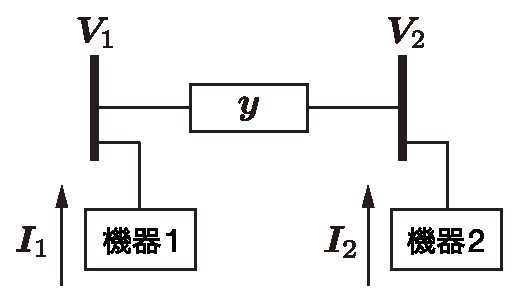
\includegraphics[width = .4\linewidth]{figs/2busex}
\medskip
\caption{\textbf{2つの母線で構成される電力系統モデル}}
\label{fig:2buspf}
\medskip
\end{figure}

\begin{例}[2つの母線で構成される電力系統モデルの潮流計算]\label{ex:2buspf}
\FIGref{fig:2buspf}の2つの母線から構成される電力系統を考えよう。
各母線には負荷または発電機が接続されているものと考えるが,潮流計算では接続される機器の種類を具体的に指定する必要はない。

2つの母線を結ぶ送電線のアドミタンスを$\bm{y}\in \mathbb{C}$とする。
基本的な送電線モデルを採用するとき,母線の電圧フェーザと電流フェーザには
\begin{align}\label{eq:exyIV}
\mat{
\bm{I}_1^{\star}\\
\bm{I}_2^{\star}
}
=
\mat{
\bm{y} & -\bm{y} \\
-\bm{y} & \bm{y}
}
\mat{
\bm{V}_1^{\star}\\
\bm{V}_2^{\star}
}
\end{align}
の関係が成り立つ。
ただし,定常状態における値であることを明示するために「${\star}$」をつけて表記した。
ここで,
式\ref{eq:defPQVIi2}の関係を用いて電流フェーザを消去すれば,式\ref{eq:exyIV}と等価な連立方程式が,定常状態における有効電力,無効電力,電圧フェーザを用いて
\begin{subequations}\label{eq:PQpf}
\begin{align}\label{eq:PQcom}
\simode{
P_1^{\star} + \bm{j} Q_1^{\star} &= 
\overline{\bm{y}} \left( 
 |\bm{V}_1^{\star}|^2 
-  |\bm{V}_1^{\star}| |\bm{V}_2^{\star}| e^{ \bm{j} (\angle \bm{V}_1^{\star}- \angle \bm{V}_2^{\star})}
\right) \\
P_2^{\star} + \bm{j} Q_2^{\star} &= 
\overline{\bm{y}} \left( 
 |\bm{V}_2^{\star}|^2
 - |\bm{V}_1^{\star}| |\bm{V}_2^{\star}| e^{ \bm{j} (\angle \bm{V}_2^{\star} - \angle \bm{V}_1^{\star})}
\right)
}
\end{align}
のように得られる。
潮流計算の目的は,この連立方程式を満たす1組の
\[
(P_1^{\star},Q_1^{\star}, |\bm{V}_1^{\star}|, \angle \bm{V}_1^{\star}, P_2^{\star},Q_2^{\star},|\bm{V}_2^{\star}|, \angle \bm{V}_2^{\star})
\]
を定めることである。

送電線のコンダクタンスとサセプタンスを
\[
g:= \real[\bm{y}],\qquad
b:= \imag[\bm{y}]
\]
と表す。
このとき,式\ref{eq:PQcom}の実部と虚部に関する方程式を考えると
\begin{align}\label{eq:PQreal}
\simode{
P_1^{\star} &= g |\bm{V}_1^{\star}|^2  
-   g |\bm{V}_1^{\star}| |\bm{V}_2^{\star}| \sfcos \angle \bm{V}_{12}^{\star}
 - b |\bm{V}_1^{\star}| |\bm{V}_2^{\star}| \sfsin \angle \bm{V}_{12}^{\star}
\\
P_2^{\star} &= g |\bm{V}_2^{\star}|^2  
-  g |\bm{V}_1^{\star}| |\bm{V}_2^{\star}| \sfcos \angle \bm{V}_{21}^{\star}
 - b |\bm{V}_1^{\star}| |\bm{V}_2^{\star}| \sfsin \angle \bm{V}_{21}^{\star}
\\
Q_1^{\star} &= - b |\bm{V}_1^{\star}|^2  
+ b |\bm{V}_1^{\star}| |\bm{V}_2^{\star}| \sfcos \angle \bm{V}_{12}^{\star} 
 - g |\bm{V}_1^{\star}| |\bm{V}_2^{\star}| \sfsin \angle \bm{V}_{12}^{\star}
\\
Q_2 &= - b |\bm{V}_2^{\star}|^2  
+ b |\bm{V}_1^{\star}| |\bm{V}_2^{\star}| \sfcos \angle \bm{V}_{21}^{\star} 
- g |\bm{V}_1^{\star}| |\bm{V}_2^{\star}| \sfsin \angle \bm{V}_{21}^{\star}
}
\end{align}
という4本の連立方程式が得られる。
\end{subequations}
ただし,$\angle \bm{V}_{ij}^{\star}$は$\angle \bm{V}_i^{\star}- \angle \bm{V}_j^{\star}$を表す。
電圧フェーザの位相は差分値のみが意味をもつため,実質的に決定すべき変数は7個である。
したがって,式\ref{eq:PQreal}の方程式には3変数分の自由度が存在する。
これらを決定するためには,例えば,$(|\bm{V}_1^{\star}|,|\bm{V}_2^{\star}|,\angle \bm{V}_{12}^{\star})$の3変数を適当な値に指定すれば良い。
これにより,残りの$(P_1^{\star},P_2^{\star},Q_1^{\star},Q_2^{\star})$は式\ref{eq:PQreal}の右辺を計算するだけで決定される。
しかしながら,この方法では,各母線の電圧フェーザは任意の値に設定できる一方で,各母線に供給される電力や消費される電力を任意の値に設定することができない。
すなわち,どれが電力を消費する負荷母線であり,どれが電力を供給する発電機母線であるかを指定することができない。
したがって,現実的な設定で数値シミュレーションを実行するためには,指定した有効電力や無効電力の値を実現するように電圧フェーザの値を適切に定めることがしばしば必要となる。

例えば,母線に供給される有効電力がバランスした
\begin{align}\label{eq:P1P2ex}
P_1^{\star}=1,\qquad
P_2^{\star}=-1
\end{align}
を実現する$(|\bm{V}_1^{\star}|,|\bm{V}_2^{\star}|,\angle \bm{V}_{12}^{\star})$を求めることを考えてみよう。
これは,母線1に接続された機器が供給する有効電力と母線2に接続された機器が消費する有効電力が,定常状態においてどちらも1である場合に,電圧フェーザの分布を求めることに相当する。
式\ref{eq:PQreal}の$P_1^{\star}$と$P_2^{\star}$に関する方程式を足し上げれば,$P_1^{\star}$と$P_2^{\star}$の和は0であることから
\begin{align*}
\spliteq{
0 &= g \Bigl\{
 |\bm{V}_1^{\star}|^2 + |\bm{V}_2^{\star}|^2 
- 2 |\bm{V}_1^{\star}| |\bm{V}_2^{\star}| \sfcos \angle \bm{V}_{12}^{\star}
\Bigr\}\\
&=
g \Bigl\{
\left( |\bm{V}_1^{\star}| - |\bm{V}_2^{\star}| \right)^2 
+ 2 |\bm{V}_1^{\star}| |\bm{V}_2^{\star}| \bigl( 1-\sfcos \angle \bm{V}_{12}^{\star} \bigr)
\Bigr\}
}
\end{align*}
を得る。
ここで,現実的な潮流状態では,母線の電圧フェーザの位相差である$ \angle \bm{V}_{12}^{\star}$は$\pm \tfrac{\pi}{2}$の範囲内であることに注意されたい。
なお,発電機の偏角差や母線の電圧フェーザの位相差が$\pm \tfrac{\pi}{2}$の範囲を超えてしまうと正弦関数の傾きが反転するため,非現実的な有効電力の送電特性となる。
%\footnote{
%発電機の偏角差や母線の電圧フェーザの位相差が$\pm \tfrac{\pi}{2}$の範囲を超えてしまうと正弦関数の傾きが反転するため,非現実的な有効電力の送電特性となる。
%}。
このことから,$\bm{y}$の実部である送電線のコンダクタンス$g$が0でない場合には,この方程式を満たす電圧フェーザは,必ず
\begin{align}\label{eq:Vequal}
|\bm{V}_1^{\star}| = |\bm{V}_2^{\star}|,\qquad
\angle \bm{V}_{12}^{\star} =0
\end{align}
を満たさなければならない。
しかしながら,式\ref{eq:Vequal}は
$P_1^{\star}$と$P_2^{\star}$がともに0であることを意味する。
したがって,$g$が0でない限りは,式\ref{eq:P1P2ex}を満たす定常潮流状態は実現不可能であることが結論づけられる。
これは,送電線のコンダクタンス成分(抵抗成分)により送電損失が生じるため,式\ref{eq:P1P2ex}の設定では電力の需給が系統全体でバランスしないことを表している。
このように,「すべての有効電力やすべての無効電力を特定の値に指定してしまうと,式(\ref{eq:PQpf})を満たす変数が存在しない場合があること」に注意が必要である。

以下では,簡単化のため,送電線のコンダクタンス$g$が0であると仮定してみよう。
また,対地静電容量は十分に小さく,サセプタンス$b$は負であると仮定する。
このとき
\begin{align*}
P_1^{\star} = -b  |\bm{V}_1^{\star}| |\bm{V}_2^{\star}| \sfsin \angle \bm{V}_{12}^{\star}, \qquad
P_2^{\star}  =   b |\bm{V}_1^{\star}| |\bm{V}_2^{\star}| \sfsin \angle \bm{V}_{12}^{\star}
\end{align*}
であることから,電圧フェーザの分布は$P_1^{\star}$と$-P_2^{\star}$が等しいものでなければならない。
例えば,式\ref{eq:P1P2ex}の値を指定する場合には
\begin{align*}\textstyle
|\bm{V}_1^{\star}|=\sqrt{
\frac{2}{|b|}
}
,\qquad
 |\bm{V}_2^{\star}| 
=
\sqrt{
\frac{2}{|b|}
}
\end{align*}
のように電圧フェーザの絶対値を指定することにより,位相差は
\begin{align*}
\angle \bm{V}_{12}^{\star} = \frac{\pi}{6}
\end{align*}
と定められる。
既に3変数以上の値が定められているため,無効電力は
\begin{align*}
Q_1^{\star} = 2 -\sqrt{3},\qquad
Q_2^{\star} = 2 -\sqrt{3}
\end{align*}
のように自動的に値が定まる。
\end{例}


例\ref{ex:2buspf}で示されたように,与えられた送電網のアドミタンス行列$\bm{Y}$に対して,定常状態における$2N$本の連立方程式
\begin{align}\label{eq:PQVgenst}
\simode{
P_1^{\star} + \bm{j} Q_1^{\star} &= 
\sum_{j=1}^{N} \overline{\bm{Y}}_{1j} |\bm{V}_1^{\star}| |\bm{V}_j^{\star} | e^{\bm{j} (\angle \bm{V}_1^{\star} - \angle \bm{V}_j^{\star} )} \\ 
& \; \;  \vdots \\
P_N^{\star} + \bm{j} Q_N^{\star} &= 
\sum_{j=1}^{N} \overline{\bm{Y}}_{Nj} |\bm{V}_N^{\star}| |\bm{V}_j^{\star} | e^{\bm{j} (\angle \bm{V}_N^{\star} - \angle \bm{V}_j^{\star} )}
}
\end{align}
を満たす,$4N$個の定数の組
\begin{align}\label{eq:pfconst}
\bigl(
P_1^{\star},Q_1^{\star},|\bm{V}_1^{\star}|,\angle \bm{V}_1^{\star},
\ldots,
P_N^{\star},Q_N^{\star},|\bm{V}_N^{\star}|,\angle \bm{V}_N^{\star},
\bigr)
\end{align}
を1つ定める手続きが潮流計算である。
ただし,電圧フェーザの位相は相対的な値のみが意味をもつため,実質的に定めるべき変数は$(4N-1)$個である。
\ref{sec:numstep}節で上述したように,潮流計算は,系統全体で需要と供給をバランスすることが可能な電力系統モデルの平衡点を求める手続きであると解釈できる。
なお,このプロセスにおいては,発電機や負荷などの各機器の特性は考慮されておらず,各母線に対する入出力の定常値のみを求めている。
正確には,\ref{sec:numstep}節におけるステップBの計算を行うことで,微分代数方程式系の内部状態に関する平衡点が1つ定まる。
ステップBの計算は,\ref{sec:paradef}節で後述する。

%例えば,\ref{sec:loadpr}節における負荷の定インピーダンスモデルは,$(P_i,Q_i)$と$|\bm{V}_i|$の間に
%\begin{align*}
%P_i + \bm{j} Q_i = -\frac{1}{\overline{\bm{z}}_{{\rm load}i}} |\bm{V}_i|^2
%\end{align*}
%という代数的な関係を与える。
%すなわち,$\bm{z}_{{\rm load}i}$が所与の定数である場合には,2本の方程式が式\ref{eq:PQVgen}に追加されることを意味している。
%負荷が定電流モデルや定電力モデルで記述されている場合も同様である。
%\red{しかしながら.... なぜそうしない?データシートで与えられているのが普通PQだから?}
%ただし,式(\ref{eq:gendynVI})の発電機の定常状態は機械入力$P_{{\rm mech}i}$と界磁入力$V_{{\rm field}i}$という別の2変数にも依存するため,発電機の動特性に由来する方程式を潮流計算で考慮する必要はない。
%このことは\ref{sec:stagen}節で後述する。




\subsection{定常的な潮流状態の数値的な探索手法}


一般に電気学会標準モデル\cite{ieejstandardmodel},IEEE 39母線系統モデル\cite{athay1979practical},IEEE 68母線系統モデル\cite{singh2013ieee}などには,各送電線のインピーダンス値に加えて,各発電機母線に供給される電力や各負荷母線で消費される電力の標準的な値がデータシートとして与えられている。
それらの標準的な値に基づき$2N$個の変数を指定することによって,残りの変数を数値的に探索することができる。


データシートには,各負荷母線で消費される有効電力と無効電力の値,および,各発電機母線に供給される有効電力の値とその母線における電圧フェーザの絶対値が与えられているのが一般的である。
したがって,それらの値を用いることにより,$2N$個の定常値をあらかじめ指定することができる。
しかしながら,例\ref{ex:2buspf}で示されているように,すべての母線における有効電力の定常値を事前に指定してしまうと,送電損失の影響によって,残りの変数をいかなる値にしても式\ref{eq:PQVgen}の連立方程式を満たせなくなってしまう。
例えば,一部の負荷母線における有効電力や無効電力の値をデータシートとは異なる定常値に指定すると,発電機母線に供給されるべき有効電力や無効電力の定常値も変化すると同時に,送電網を流れる電力や母線電圧フェーザの定常値も変化するため,系統全体での送電損失の合計値も変化する。
したがって,すべての発電機母線における有効電力の定常値を事前に指定してしまうと,式\ref{eq:PQVgen}の連立方程式が一般に可解とならない。


この問題を解決するための代表的な方策は,\textbf{スラック母線}(slack bus)\index{ すらっくぼせん@スラック母線}と呼ばれる特別な発電機母線を1つ導入することである。
スラック母線では,有効電力を指定する代わりに,電圧フェーザの位相を指定する。
このとき,各母線における電圧フェーザの位相は相対的な値のみが意味をもつため,スラック母線の位相の定常値を0に指定しても一般性を失わない。
結果として,系統全体での送電損失の値に整合するように,スラック母線における有効電力が自動的に決定される。
以上の手順は,つぎのようにまとめられる。

\medskip
\begin{breakbox}
\begin{itemize}
\item[(a)] データシートに基づき,スラック母線には$(|\bm{V}_{i_0}^{\star}|,\angle \bm{V}_{i_0}^{\star})$の値,それ以外の発電機母線には$(P_i^{\star},|\bm{V}_{i}^{\star}|)_{i \in \mathcal{I}_{\rm G}\setminus\{i_0\} }$の値,負荷母線には$(P_i^{\star},Q_i^{\star})_{i \in \mathcal{I}_{\rm L}}$の値を指定する。
\item[(b)] 式\ref{eq:PQVgen}の連立方程式が満たされるように,その他の変数を数値的に探索する。
\end{itemize}
\end{breakbox}
\medskip

なお,$\mathcal{I}_{\rm G}$は発電機母線の添字集合,$\mathcal{I}_{\rm L}$は負荷母線の添字集合,$i_0 \in \mathcal{I}_{\rm G}$はスラック母線の添字を表す。
機器が接続されていない母線は,消費される有効電力と無効電力が0である負荷母線として扱う。

%参考として,3つの発電機母線(母線1,母線2,母線3)と2つの負荷母線(母線4,母線5)から構成される電力系統モデルの例を\FIGref{fig:powerflow}に示す。
%ここでは発電機母線1をスラック母線に設定しており,その他の母線には,有効電力や無効電力,母線電圧フェーザの絶対値などが指定されている。
%
%\begin{figure}[t]
%\centering
%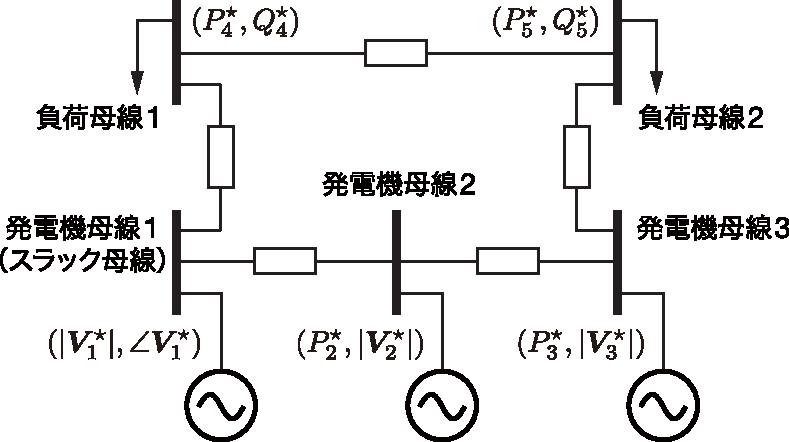
\includegraphics[width = .7\linewidth]{figs/powerflow}
%\medskip
%\caption{\textbf{3発電機母線と2負荷母線の潮流計算}}
%\label{fig:powerflow}
%\medskip
%\end{figure}


\begin{table}[h]
\medskip
\caption{\textbf{データシートと潮流計算結果(1)}} \label{table:pflow1}
 \centering
  {
  \begin{minipage}{0.49\linewidth}
    \centering
  \begin{tabular}{|c|c|c|c|c|c|c|}
   \hline
 &  母線1 & 母線2 & 母線3 \\
   \hline 
   $P_i^{\star}$ & 0.5 & $-3$ & \\
   \hline
   $Q_i^{\star}$ &  & 0 & \\
   \hline
   $|\bm{V}_i^{\star}|$ & 2 & & 2 \\
   \hline
   $\angle \bm{V}_i^{\star}$ & & & 0 \\
   \hline
  \end{tabular}
  \subcaption{データシート}
  \end{minipage}
  \begin{minipage}{0.49\linewidth}
    \centering
  \begin{tabular}{|c|c|c|c|c|c|c|}
   \hline
 &  母線1 & 母線2 & 母線3 \\
   \hline 
   $P_i^{\star}$ & & & 2.5006 \\
   \hline
   $Q_i^{\star}$ & 0.0157 & & 0.1388 \\
   \hline
   $|\bm{V}_i^{\star}|$ & & 1.9969 & \\
   \hline
   $\angle \bm{V}_i^{\star}$ & $-0.0490$ & $-0.0596$ & \\
   \hline
  \end{tabular}
   \subcaption{潮流計算結果}
  \end{minipage}
  }
\end{table}


\begin{table}[h]
\medskip
\caption{\textbf{データシートと潮流計算結果(2)}} \label{table:pflow2}
 \centering
  {
  \begin{minipage}{0.49\linewidth}
    \centering
  \begin{tabular}{|c|c|c|c|c|c|c|}
   \hline
 & 母線1 & 母線2 & 母線3 \\
   \hline 
   $P_i^{\star}$ &  & $-3$ & 0.5 \\
   \hline    
   $Q_i^{\star}$ &  & 0 & \\
   \hline
   $|\bm{V}_i^{\star}|$ & 2 & & 2 \\
   \hline
   $\angle \bm{V}_i$ & 0 & &  \\
   \hline
  \end{tabular}
   \subcaption{データシート}
  \end{minipage}
  \begin{minipage}{0.49\linewidth}
    \centering
  \begin{tabular}{|c|c|c|c|c|c|c|}
   \hline
 &  母線1 & 母線2 & 母線3 \\
   \hline 
   $P_i^{\star}$ & 2.5158 & &  \\
   \hline
   $Q_i^{\star}$ & $-0.0347$ & & 0.1759 \\
   \hline
   $|\bm{V}_i^{\star}|$ & & 1.9918 & \\
   \hline
   $\angle \bm{V}_i^{\star}$ & & $-0.0538$ & $-0.0419$ \\
   \hline
  \end{tabular}
  \subcaption{潮流計算結果}
  \end{minipage}
  }
\end{table}



\begin{例}[データシートに基づく潮流計算]\label{ex:pf3bus}
例\ref{ex:derY}で議論した3母線で構成される電力系統モデルを考えよう。
式\ref{eq:exY}の送電網のアドミタンス行列に対して,2つの送電線のアドミタンス値は
\begin{align}\label{eq:rightlossless}
\bm{y}_{12} = 1.3652 - \bm{j} 11.6041, \qquad
\bm{y}_{23} =  - \bm{j} 10.5107
\end{align}
に設定する。
母線2と母線3を結ぶ送電線のコンダクタンス($\bm{y}_{23}$の実部)は0に設定されており,その送電線における有効電力の送電損失は0となることに注意されたい。

まず,母線1が発電機母線,母線2が負荷母線,母線3がスラック母線である場合を考える。
具体的には,\TABref{table:pflow1}(a)に示されている値が各母線に指定されているものとする。
このとき,式\ref{eq:PQVgenst}の連立方程式を満たす変数の組は,\TABref{table:pflow1}(b)のように求められる。
この場合の送電損失は
\[
P_1^{\star} + P_2^{\star} + P_3^{\star} = 6.2562\times 10^{-4},
\qquad 
Q_1^{\star} + Q_2^{\star} + Q_3^{\star} =1.5450  \times 10^{-1}
\]
となる。
負荷の消費電力に対する送電損失の比率は0.02\%程度と非常に小さい。
有効電力の送電損失が小さい理由は,
母線2の負荷で消費される有効電力が3~[pu]であるのに対して,その大半の約2.5~[pu]を母線3の発電機から供給しており,母線1の発電機からは0.5~[pu]しか供給していないためである。
すなわち,母線2で消費される有効電力の大半を送電損失が生じない右側の送電線を用いて供給している。

つぎに,母線1がスラック母線,母線2が負荷母線,母線3が発電機母線である場合として,\TABref{table:pflow2}(a)のように各母線の変数を指定する。
このときの潮流計算の結果は\TABref{table:pflow2}(b)となる。
この場合の送電損失は
\[
P_1^{\star} + P_2^{\star} + P_3^{\star} = 1.5826 \times 10^{-2},
\qquad 
Q_1^{\star} + Q_2^{\star} + Q_3^{\star} =1.4120  \times 10^{-1}
\]
となる。
この場合の負荷の消費電力に対する送電損失の比率は約0.52\%である。
先の例と比較して,有効電力の送電損失が大きくなっていることがわかる。
これは,送電損失が生じる左側の送電線を使って,母線2で消費される有効電力の大半を供給したことに起因する。
一方で,無効電力の損失は,先の例と比較して小さくなっていることもわかる。
\end{例}

例\ref{ex:pf3bus}から,求められる潮流状態によって,系統全体の送電損失の大きさが異なることがわかる。
一般に,コンダクタンス成分(抵抗成分)が大きい送電線を使って消費電力を供給する場合に,有効電力の送電損失が大きくなる。
送電損失が大きくなるほど,同じ有効電力の消費量を供給するために必要な発電量が大きくなるため,発電費用などの経済コストも大きくなってしまう。

一方で,経済コストの低い定常潮流状態が,必ずしも安定度の高い平衡点ではない点にも注意が必要である。
したがって,経済性や安定度などに関するトレードオフを考慮して,より良い平衡点を探索することが実応用では重要となる。
そのようなより良い平衡点探索のプロセスは,電力系統工学では\textbf{最適潮流計算}(optimal power flow calculation)\index{ さいてきちょうりゅうけいさん@最適潮流計算}と呼ばれる。
本書では,平衡点の選び方と安定度の関係を\ref{sec:staana}章や\ref{ch:stabcont}章で議論する。

\subsection{アドミタンス行列と送電損失の関係\advanced}

以下では,$N$個の母線で構成される一般的な送電網に対して,任意の潮流状態に関する送電損失の数学的表現を導出する。
アドミタンス行列$\bm{Y}$の実部と虚部であるコンダクタンス行列$G$とサセプタンス行列$B$がそれぞれ対称である場合には,適当な定数$\phi_{ij}=\phi_{ji}$,$\psi_{ij}=\psi_{ji}$を用いて
%\begin{align}\label{eq:GBrep}
%\spliteq{
%G
%& =
%\mat{
%  \sum_{j=1}^{N} \phi_{1j} & -\phi_{12} & \cdots & -\phi_{1N}\\
%  -\phi_{21} & \sum_{j=1}^{N} \phi_{2j} & \cdots & -\phi_{2N}\\
%  \vdots & \vdots & \ddots & \vdots\\
%  -\phi_{N1} & -\phi_{N2} & \cdots & \sum_{j=1}^{N} \phi_{Nj}
%},
%\\
%B
%& =
%-\mat{
%  \sum_{j=1}^{N} \psi_{1j} & -\psi_{12} & \cdots & -\psi_{1N}\\
%  -\psi_{21} & \sum_{j=1}^{N} \psi_{2j} & \cdots & -\psi_{2N}\\
%  \vdots & \vdots & \ddots & \vdots\\
%  -\psi_{N1} & -\psi_{N2} & \cdots & \sum_{j=1}^{N} \psi_{Nj}
%}
%}
%\end{align}
\begin{align}\label{eq:GBrep}
G_{ij} =
\left\{
\begin{array}{cl}
\textstyle \sum_{j=1}^{N} \phi_{ij}, & i=j \\
-\phi_{ij}, & i\neq j 
\end{array}
\right.
\quad
B_{ij}  =
\left\{
\begin{array}{cl}
\textstyle - \sum_{j=1}^{N} \psi_{ij}, & i=j \\
\psi_{ij}, & i\neq j 
\end{array}
\right.
\end{align}
の形式で書き表すことができる。
ただし,$G_{ij}$と$B_{ij}$はそれぞれ,コンダクタンス行列$G$とサセプタンス行列$B$の第$(i,j)$要素を表す。
式\ref{eq:GBrep}は
\[
\phi_{ii}:= \sum_{j=1}^N G_{ij},\qquad
\phi_{ij}:=-G_{ij},\qquad 
\psi_{ii}:= - \sum_{j=1}^N B_{ij},\qquad 
\psi_{ij}:=B_{ij}
\]
と定義していることに等しい。
この表現を用いるとつぎの事実が示される。

\begin{定理}[送電損失の母線電圧フェーザによる表現]
\label{thm:PQ}
式\ref{eq:PQVgen}に対して,系統全体での有効電力と無効電力の送電損失として
\begin{align}
L_{P}(t) := P_1(t) +\cdots P_N(t)
,\qquad
L_Q(t) := Q_1(t) +\cdots Q_N(t)
\end{align}
を定義する。
これらの送電損失は
\begin{align}\label{eq:LPLQ}
\spliteq{
L_P(t) &= \sum_{i=1}^N \phi_{ii} |\bm{V}_{i}(t)|^2  +
\sum_{i=1}^N \sum_{j=i+1}^N
\phi_{ij} 
W\bigl(\bm{V}_i(t),\bm{V}_j(t)\bigr)
\\
L_Q(t) &= \sum_{i=1}^N \psi_{ii} |\bm{V}_{i}(t)|^2  +
\sum_{i=1}^N \sum_{j=i+1}^N
\psi_{ij} 
W\bigl(\bm{V}_i(t),\bm{V}_j(t)\bigr)
}
\end{align}
で与えられる。
ただし
\[
W(\bm{V}_i,\bm{V}_j):=
\left( |\bm{V}_i| - |\bm{V}_j| \right)^2 
+ 2 |\bm{V}_i| |\bm{V}_j| \bigl\{ 1-\sfcos (\angle \bm{V}_i- \angle \bm{V}_j) \bigr\}
\]
とする。
\end{定理}

\begin{証明}
表記の簡単化のため,時刻$t$は省略する。
また,$\angle\bm{V}_i- \angle \bm{V}_j$を$\angle \bm{V}_{ij}$と表す。
式\ref{eq:PQVgen}より,$\bm{Y}_{ij}= G_{ij} + \bm{j} B_{ij}$に対して,$\bm{Y}_{ij}=\bm{Y}_{ji}$より
\begin{align*}
\spliteq{
\sum_{i=1}^N (P_i + \bm{j} Q_i)
 & =
\sum_{i=1}^N \overline{\bm{Y}}_{ii} |\bm{V}_i|^2
+
\sum_{i=1}^N \sum_{j=i+1}^N
\overline{\bm{Y}}_{ij}
|\bm{V}_i| |\bm{V}_j| 
\left(e^{ \bm{j} \angle \bm{V}_{ij} } + e^{ \bm{j} \angle \bm{V}_{ji} } \right) \\
 & =
\sum_{i=1}^N \overline{\bm{Y}}_{ii} |\bm{V}_i|^2
+
2
\sum_{i=1}^N \sum_{j=i+1}^N
\overline{\bm{Y}}_{ij}
|\bm{V}_i| |\bm{V}_j| 
\sfcos \angle \bm{V}_{ij}
}
\end{align*}
が成り立つ。
したがって,式\ref{eq:GBrep}の$G_{ij}$と$B_{ij}$の表記を用いれば
\begin{align*}
\spliteq{
L_P &= 
\sum_{i=1}^N \left(
\sum_{j=1}^N \phi_{ij}
\right)
|\bm{V}_i|^2
-
2
\sum_{i=1}^N \sum_{j=i+1}^N
\phi_{ij}
|\bm{V}_i| |\bm{V}_j| 
\sfcos \angle \bm{V}_{ij} \\
L_Q &= 
\sum_{i=1}^N \left(
\sum_{j=1}^N \psi_{ij}
\right)
|\bm{V}_i|^2
-
2
\sum_{i=1}^N \sum_{j=i+1}^N
\psi_{ij}
|\bm{V}_i| |\bm{V}_j| 
\sfcos \angle \bm{V}_{ij}
}
\end{align*}
が得られる。
ここで,$L_P$の第1項に注目すると,$\phi_{ij}=\phi_{ji}$であることから
\[\sum_{i=1}^N 
\sum_{j=1}^N \phi_{ij}
|\bm{V}_i|^2 = 
\sum_{i=1}^N 
\phi_{ii}|\bm{V}_i|^2
+
\sum_{i=1}^N 
\sum_{j=i+1}^N \phi_{ij}
|\bm{V}_i|^2
+
\sum_{i=1}^N 
\sum_{j=i+1}^N \phi_{ij}
|\bm{V}_j|^2
\]
がわかる。
これを用いて$L_P$の第1項を書き換えれば
\begin{align*}
\spliteq{
L_P &= 
\sum_{i=1}^N 
\phi_{ii}|\bm{V}_i|^2
+
\sum_{i=1}^N 
\sum_{j=i+1}^N \phi_{ij}
\left(
|\bm{V}_i|^2
+
|\bm{V}_j|^2
-
2 |\bm{V}_i| |\bm{V}_j| 
\sfcos \angle \bm{V}_{ij}
\right)
\\
&= 
\sum_{i=1}^N 
\phi_{ii}|\bm{V}_i|^2
+
\sum_{i=1}^N 
\sum_{j=i+1}^N \phi_{ij}
\left\{
\left(
|\bm{V}_i|
-
|\bm{V}_j|
\right)^2
+
2 |\bm{V}_i| |\bm{V}_j| 
(1-
\sfcos \angle \bm{V}_{ij}
)
\right\}
}
\end{align*}
が得られる。
したがって,$L_P$は式\ref{eq:LPLQ}の形式で表せることがわかる。
同様の手順により,$L_Q$は式\ref{eq:LPLQ}の形式で表せることもわかる。
\end{証明}

定理\ref{thm:PQ}は,例\ref{ex:2buspf}で示されている2母線の電力系統における電力損失の議論が,任意の個数の母線から構成される電力系統にも同様に一般化できることを示している。
ここで,\ref{sec:admathp}節のようにアドミタンス行列$\bm{Y}$を
\[
\bm{Y}=\bm{Y}_0 + \bm{j} \sfdiag(\Cgi)_{i\in \{1,\ldots,N\} }
\]
と表す場合には,$\bm{Y}_0 \mathds{1}$は0であること,すなわち,$\bm{Y}_0$の実部と虚部に対して各々すべての行の和は0であることから
\[
\phi_{ii}=0,\qquad
\psi_{ii}= - \Cgi
\]
となる。
また,各送電線のコンダクタンスは非負であり,サセプタンスは負であることから,すべての$i\neq j$に対して,$\phi_{ij} $と$\psi_{ij}$は非負である。
したがって,$\phi_{ij}$が0でない限りは,母線$i$と母線$j$の間で有効電力を送電する場合に必ず損失が生じることがわかる。
これにより,系統全体での有効電力の送電損失$L_P(t)$は,任意の時刻$t$で正であることがわかる。
同様に,$\Cgi$が十分に小さい場合,すなわち,送電線の対地静電容量が十分に小さい場合には,無効電力の損失$L_Q(t)$も正であることがわかる。
言い換えれば,キャパシタンスの特性をもつ機器を母線に接続することは,無効電力の損失を減らす効果を与える。



\section{所与の潮流状態を実現する各機器のパラメータ設定}\label{sec:paradef}

本節では,\ref{sec:numstep}節のステップBとして説明された,潮流計算の結果に整合するように発電機の内部状態の定常値や外部入力値,負荷のパラメータ値を逆算する方法を説明する。


\subsection{所望の電力供給を実現する発電機の定常状態}\label{sec:stagen}

\ref{sec:genfund}節における電圧フェーザを入力とする発電機モデルを考えよう。
表記の簡単化のため,添字$i$を省略して
\begin{align}\label{eq:gendif_}
\simode{
\dot{\delta}&= \omega_0  \Delta \omega\\
M   \Delta \dot{\omega}&= 
 - D \Delta\omega  
 - P
+P_{{\rm mech}}
\\
\taud \dot{E} & = 
-\tfrac{ \Xs }{ \Xt }E
+\left(
\tfrac{ \Xs }{ \Xt } -1
\right)
|\bm{V}| \sfcos (\delta - \angle \bm{V} ) 
+ V_{{\rm field}}
}
\end{align}
と表す。
ここで,有効電力と無効電力を出力とする場合には
\begin{align}\label{eq:PQout_}
P =  \frac{|\bm{V} | E}{ \Xt } \sfsin(\delta -  \angle \bm{V}), \qquad
Q =  \frac{|\bm{V}|E}{ \Xt } \sfcos (\delta - \angle \bm{V})
-\frac{|\bm{V}|^2}{ \Xt }
\end{align}
である。
%また,電流フェーザを出力とする場合には
%\begin{align}\label{eq:phVIsincosC2_}
%\spliteq{
% |\bm{I}| \sfcos (\delta -\angle \bm{I}) & =
%\frac{|\bm{V}|}{X_{{\rm q}}}  \sfsin (\delta -\angle \bm{V}) , \\
%|\bm{I}| \sfsin (\delta -\angle \bm{I})
%& = \frac{E - |\bm{V}| \sfcos (\delta -\angle \bm{V}) }{X_{{\rm q}}} 
%}
%\end{align}
%である。
ここでの目的は,潮流計算の結果として,発電機が接続される母線の有効電力,無効電力,電圧フェーザの絶対値と位相が定数で与えられた場合に,それらの値に整合する発電機の内部状態と外部入力値の定常値を求めることである。
具体的には,与えられた有効電力,無効電力,電圧フェーザの絶対値と位相の組を$(P^{\star},Q^{\star},|V^{\star}|,\angle \bm{V}^{\star})$と表すとき
\begin{align}\label{eq:P0Q0eq}
\simode{
P^{\star} &=  \tfrac{|V^{\star}| E^{\star}}{ \Xt } \sfsin(\delta^{\star} -  \angle \bm{V}^{\star}), \\
Q^{\star} & = \tfrac{|V^{\star}| E^{\star}}{ \Xt } \sfcos (\delta^{\star} -  \angle \bm{V}^{\star})
-\tfrac{|V^{\star}|^2}{ \Xt }, \\
0 & =  - P^{\star} +P_{{\rm mech}}^{\star}, \\
0 & = 
 -\tfrac{ \Xs }{ \Xt }E^{\star}
+\left(
\tfrac{ \Xs }{ \Xt }-1
\right)
|V^{\star}| \sfcos (\delta^{\star} - \angle \bm{V}^{\star})
+ V_{{\rm field}}^{\star}
}
\end{align}
の連立方程式を満たす発電機の内部状態の定常値$(\delta^{\star},E^{\star})$と外部入力の定常値$(P_{{\rm mech}}^{\star},V_{{\rm field}}^{\star})$を求めることが目的となる。
式\ref{eq:P0Q0eq}の連立方程式は,式\ref{eq:gendif_}において角周波数偏差$\Delta \omega$の定常値が0であるとした場合の平衡点に関する方程式である。
また,与えられた$(P^{\star},Q^{\star},|V^{\star}|,\angle \bm{V}^{\star})$は,各母線に対する発電機モデルの入出力値に対応している。


式\ref{eq:P0Q0eq}を満たす発電機の内部状態の定常値を具体的に計算すると
\begin{subequations}\label{eq:intssgen}
\begin{align}
\spliteq{
\delta ^{\star} &= \angle \bm{V}^{\star}
+ \sfarctan \left( \frac{P^{\star}}{Q^{\star} + \tfrac{ |\bm{V}^{\star}|^2}{ \Xt } } \right), 
\\
E^{\star} &= 
\frac{ \Xt }{ |\bm{V}^{\star}| } \sqrt{ \left( Q^{\star} + \frac{|\bm{V}^{\star}|^2}{ \Xt } \right)^2 + (P^{\star})^2 } 
}
\end{align}
となる。
また,機械入力と界磁入力の定常値は
\begin{align}\label{eq:PmVfdss}
\spliteq{
P_{{\rm mech}}^{\star} &=    P^{\star}, \\
 V_{{\rm field}}^{\star} &=  \frac{ \tfrac{ \Xs }{ |\bm{V}^{\star}| } \left\{ \left( Q^{\star} + \tfrac{|\bm{V}^{\star}|^2}{ \Xt } \right) 
\left(Q^{\star} + \tfrac{|\bm{V}^{\star}|^2}{ \Xs } \right) +(P^{\star})^2  \right\} }
{  \sqrt{ \left( Q^{\star} + \tfrac{|\bm{V}^{\star}|^2}{ \Xt } \right)^2 + (P^{\star})^2 }  }
}
\end{align}
となる。
\end{subequations}
これらの導出過程は,\ref{sec:genssPQ}節を参照されたい。

\subsection{所望の電力消費を実現する負荷のパラメータ}\label{sec:loadpara}

\ref{sec:loadpr}節で説明された負荷モデルに対して,所望の電力消費に整合するパラメータを設定する方法を説明する。
式\ref{eq:defPQVIi2}を用いて電流フェーザを消去すると,定インピーダンスモデルは
%\begin{subequations}\label{eq:lmodels}
\begin{align}\label{eq:lmodimp}
P + \bm{j} Q = -\frac{|\bm{V}|^2}{\overline{\bm{z}}_{\rm load}^{\star}} 
\end{align}
と書き表される。
ただし,母線の添字$i$は表記の簡単化のため省略した。
これは電流フェーザ$\bm{V}$を入力,有効電力$P$と無効電力$Q$を出力とした場合の負荷の定インピーダンスモデルと解釈できる。
潮流計算により定められた有効電力と無効電力の値を$P^{\star}$と$Q^{\star}$,電圧フェーザの絶対値を$|\bm{V}^{\star}|$と表せば,負荷のインピーダンス$\bm{z}_{\rm load}^{\star}$の実部(抵抗)と虚部(リアクタンス)は
\begin{align}\label{eq:lmodimppara}
\real [\bm{z}_{\rm load}^{\star}] = - \frac{ P^{\star} |\bm{V}^{\star}|^2 }{(P^{\star})^2 + (Q^{\star})^2}
,\qquad
\imag [\bm{z}_{\rm load}^{\star}] = - \frac{ Q^{\star} |\bm{V}^{\star}|^2 }{(P^{\star})^2 + (Q^{\star})^2}
\end{align}
と求められる。
同様に,定電流モデルは
\begin{align}
P + \bm{j} Q = \overline{\bm{I}}_{\rm load}^{\star} |\bm{V}|
\end{align}
と書き表されることから,負荷の電流パラメータの実部と虚部はそれぞれ
\begin{align*}
\real [\bm{I}_{\rm load}^{\star}]
 =\frac{P^{\star} }{|\bm{V}^{\star}|},\qquad
\imag [\bm{I}_{\rm load}^{\star}]
 = -\frac{ Q^{\star} }{|\bm{V}^{\star}|}
\end{align*}
と求められる。
定電力モデルは
\begin{align}
P + \bm{j} Q =
P_{{\rm load}}^{\star} + \bm{j} Q_{{\rm load}}^{\star} 
\end{align}
%\end{subequations}
であることから,明らかにそのパラメータは
\begin{align*}
P_{\rm load}^{\star}=P^{\star}
,\qquad
Q_{\rm load}^{\star}=Q^{\star}
\end{align*}
である。
これらのパラメータ値を負荷モデルに設定すれば,潮流計算によって求められた潮流状態が定常的に実現される。

\subsection{発電機の内部状態と入出力の数学的関係\advanced}\label{sec:genssPQ}

以下では,発電機の内部状態,母線に供給される有効電力と無効電力,母線の電圧フェーザの間に成り立つ関係を数学的に解析する。
ここでは,\ref{sec:genmodadv}節で扱った発電機モデルを用いる。
ただし,表記の簡単化のため,添字$i$を省略して
\begin{align}\label{eq:gendif}
\simode{
\dot{\delta}&= \omega_0  \Delta \omega\\
M   \Delta \dot{\omega}&= 
 - D \Delta\omega  
 - P
+P_{{\rm mech}}
\\
\taud \dot{E} & = 
 -\tfrac{X_{{\rm d}}}{X_{{\rm d}}'}E
+\left(
\tfrac{X_{{\rm d}}}{X_{{\rm d}}'}-1
\right)
|\bm{V}| \sfcos (\delta - \angle \bm{V} ) 
+ V_{{\rm field}}
}
\end{align}
とする。
ここで,有効電力と無効電力を出力とする場合には
\begin{align}\label{eq:PQout}
\spliteq{
P &=  \frac{|\bm{V} | E}{X_{{\rm d}}'} \sfsin(\delta -  \angle \bm{V})
-  
\left( \frac{1}{X_{{\rm d}}'}  -  \frac{1}{X_{{\rm q}}} \right)
|\bm{V}|^2 \sfsin( \delta - \angle \bm{V})\sfcos( \delta - \angle \bm{V}), \\
Q &=  \frac{|\bm{V}|E}{X_{{\rm d}}'} \sfcos (\delta - \angle \bm{V})
-|\bm{V}|^2 \left( \frac{\sfcos^2 (\delta - \angle \bm{V}) }{X_{{\rm d}}'} 
+ \frac{\sfsin^2 (\delta - \angle \bm{V})}{X_{{\rm q}}} \right)
}
\end{align}
である。
なお,$X_{{\rm d}}'$と$X_{{\rm q}}$が等しく$\Xt$であり,$X_{\rm d}$を$\Xs$に置き換えれば,\ref{sec:stagen}節で扱った発電機モデルに一致する。
また,電流フェーザを出力とする場合には
\begin{align}\label{eq:phVIsincosC2}
\spliteq{
 |\bm{I}| \sfcos (\delta -\angle \bm{I}) & =
\frac{|\bm{V}|}{X_{{\rm q}}}  \sfsin (\delta -\angle \bm{V}) , \\
|\bm{I}| \sfsin (\delta -\angle \bm{I})
& = \frac{E - |\bm{V}| \sfcos (\delta -\angle \bm{V}) }{X_{{\rm d}}'} 
}
\end{align}
である。
なお,式\ref{eq:PQout}と式\ref{eq:phVIsincosC2}は等価な出力であること,すなわち,与えられた任意の$(\delta, E, |\bm{V}|, \angle \bm{V})$に対して,$(P,Q)$と$(|\bm{I}|, \angle \bm{I})$には一対一の関係が存在することに注意されたい。

この発電機モデルに対して,つぎの事実が示される。

\begin{補題}[発電機の内部状態と入出力の関係]\label{lem:delVE}
式\ref{eq:PQout}を$\delta - \angle \bm{V}$と$E$に関する連立方程式と考えるとき,その解は
\begin{subequations}\label{eq:tandelV}
\begin{align}
\delta - \angle \bm{V} & = \sfarctan  \left( \frac{P}{Q + \tfrac{ |\bm{V}|^2}{X_{\rm q}} } \right) , \label{eq:tandelVa} \\
E &=
\frac{ \tfrac{X_{\rm d}'}{|\bm{V}| } \left\{ \left( Q + \tfrac{|\bm{V}|^2}{X_{\rm q}} \right) \left(Q + \tfrac{|\bm{V}|^2}{X_{\rm d}'} \right) +P^2  \right\} }
{  \sqrt{ \left( Q + \tfrac{|\bm{V}|^2}{X_{\rm q}} \right)^2 + P^2 }  }
\label{eq:tandelVb}
\end{align}
\end{subequations}
%\begin{align}\label{eq:tandelV}
%\spliteq{
%\delta(t) - \angle \bm{V}(t) & = \sfarctan  \left( \frac{P(t)}{Q(t) + \frac{ |\bm{V}(t)|^2}{X_{\rm q}} } \right) , \\
%E(t) &=
%\frac{ \frac{X_{\rm d}'}{|\bm{V}(t)| } \left\{ \left( Q(t) + \frac{|\bm{V}(t)|^2}{X_{\rm q}} \right) \left(Q(t) + \frac{|\bm{V}(t)|^2}{X_{\rm d}'} \right) +P^2(t)  \right\} }
%{  \sqrt{ \left( Q(t) + \frac{|\bm{V}(t)|^2}{X_{\rm q}} \right)^2 + P^2(t) }  }
%}
%\end{align}
で与えられる。
ただし,$|\bm{V}|\neq 0$とする。
逆に,式(\ref{eq:tandelV})を$P$と$Q$に関する連立方程式と考えるとき,その解は式\ref{eq:PQout}で与えられる。
\end{補題}

\begin{証明}
まず,式\ref{eq:PQout}から式(\ref{eq:tandelV})を導く。
式\ref{eq:PQout}の$P$に$\sfcos (\delta - \angle \bm{V})$を乗じ,
$Q$に$\sfsin (\delta - \angle \bm{V})$を乗じて差をとれば
\begin{align*}
P \sfcos (\delta - \angle \bm{V}) - Q \sfsin (\delta - \angle \bm{V})
= \frac{|\bm{V}|^2}{X_{\rm q}} \sfsin (\delta - \angle \bm{V}) 
\end{align*}
が得られる。
この両辺を$\sfcos (\delta - \angle \bm{V})$で割れば,式\ref{eq:tandelVa}の関係が得られる。
つぎに,式\ref{eq:tandelVb}の関係を示す。
式\ref{eq:defPQVIi2}を用いて$P$と$Q$を$\bm{I}$で書き直すと,式\ref{eq:PQout}は式\ref{eq:phVIsincosC2}に等価変形される。
また,これは
\begin{align}\label{eq:tmpVE}
|\bm{V}|e^{\bm{j}(\delta - \angle \bm{V})}=E
-X_{\rm d}' |\bm{I}| \sfsin (\delta - \angle \bm{I})
+ 
\bm{j} X_{\rm q} 
|\bm{I}| \sfcos (\delta - \angle \bm{I})
\end{align}
と等価である。
式\ref{eq:tandelVa}の関係を複素数で表現すると
\begin{align*}
\frac{ e^{\bm{j}(\delta - \angle \bm{V})} - e^{-\bm{j}(\delta - \angle \bm{V})}}
{e^{\bm{j}(\delta - \angle \bm{V})} + e^{-\bm{j}(\delta - \angle \bm{V})}}
= 
\underbrace{
\frac{P}{Q + \tfrac{ |\bm{V}|^2}{X_{\rm q}} }
}_{\alpha}
 \bm{j}
\end{align*}
であることから
\begin{align*}
e^{-\bm{j}(\delta - \angle \bm{V})} = \frac{1-\alpha \bm{j}}{1+\alpha \bm{j}}
e^{\bm{j}(\delta - \angle \bm{V})}
\end{align*}
がわかる。
したがって,式\ref{eq:defPQVIi2}を等価変形した
\begin{align}\label{eq:IVPQ}
|\bm{I}|e^{\bm{j}(\delta - \angle \bm{I})} = \frac{P+\bm{j}Q}{|\bm{V}|}  
e^{\bm{j}(\delta - \angle \bm{V})}
\end{align}
について,その複素共役を考えることにより
\begin{align}\label{eq:IVPQc}
|\bm{I}|e^{-\bm{j}(\delta - \angle \bm{I})} = \frac{P-\bm{j}Q}{|\bm{V}|}  
\cdot \frac{1-\alpha \bm{j}}{1+\alpha \bm{j}}
e^{\bm{j}(\delta - \angle \bm{V})}
\end{align}
を得る。
式\ref{eq:IVPQ}と式\ref{eq:IVPQc}から
\begin{align*}
|\bm{I}| \sfsin (\delta - \angle \bm{I})
& =
\frac{1}{|\bm{V}|} \cdot
\frac{\alpha P +Q}{ 1+\alpha \bm{j} }e^{\bm{j}(\delta - \angle \bm{V})}, \\
|\bm{I}| \sfcos (\delta - \angle \bm{I})
& =
\frac{1}{|\bm{V}|} \cdot
\frac{ P - \alpha Q}{ 1+\alpha \bm{j} }e^{\bm{j}(\delta - \angle \bm{V})}
\end{align*}
がわかる。
これらを式\ref{eq:tmpVE}に代入することによって,$\bm{I}$を$P$と$Q$で改めて書き直せば,式\ref{eq:tandelVa}の関係が成り立つとき,式\ref{eq:PQout}が
\begin{align}\label{eq:Etran}
E=
\frac{X_{\rm d}'}{|\bm{V}| } 
\left\{
\left(Q + \frac{|\bm{V}|^2}{X_{\rm q}} \right) \left(Q + \frac{|\bm{V}|^2}{X_{\rm d}'} \right) +P^2
\right\}
\frac{  Q + \tfrac{|\bm{V}|^2}{X_{\rm q}} - \bm{j} P }
{   \left( Q + \tfrac{|\bm{V}|^2}{X_{\rm q}} \right)^2 + P^2   }
e^{\bm{j}(\delta - \angle \bm{V})}
\end{align}
と等価であることがわかる。
ここで,式\ref{eq:tandelVa}の関係から
\begin{align*}
Q + \frac{|\bm{V}|^2}{X_{\rm q}} - \bm{j} P
= 
\left|Q + \frac{|\bm{V}|^2}{X_{\rm q}} - \bm{j} P \right|
e^{-\bm{j}(\delta - \angle \bm{V})}
\end{align*}
が成り立つことがわかる。
さらに
\[
|E|=E
,\qquad
\left( Q + \frac{|\bm{V}|^2}{X_{\rm q}} \right)^2 + P^2
=
\left|Q + \frac{|\bm{V}|^2}{X_{\rm q}} - \bm{j} P \right|^2
\]
であることから,式\ref{eq:tandelVb}の関係が得られる。

逆の手順をたどって,式(\ref{eq:tandelV})から式\ref{eq:PQout}を導く。
式\ref{eq:tandelVa}の関係を用いると,式\ref{eq:tandelVb}の$E$は式\ref{eq:Etran}の$E$で書き換えられる。
前述のように,式\ref{eq:tandelVa}の関係が成り立つとき,式\ref{eq:Etran}は式\ref{eq:PQout}と等価である。
\end{証明}

補題\ref{lem:delVE}は,変数の組$(\delta - \angle \bm{V},E)$と組$(P,Q)$の間に一対一の関係があることを示している。
特に,発電機の入出力である$(|\bm{V}|,\angle \bm{V})$や$(P,Q)$から,発電機の内部状態である$(\delta,E)$を一意的に逆算できることを示している。
なお,式(\ref{eq:tandelV})の関係は定常状態,過渡状態に関わらず任意の時刻$t$で成り立つことに注意されたい。

つぎの定理は,発電機の定常状態において,入力,出力,内部状態の間に成り立つ関係を与える。

\begin{定理}[定常状態における発電機の内部状態と入出力の関係]
\label{thm:stst}
式\ref{eq:gendif}および式\ref{eq:PQout}の発電機モデルを考える。
ある実定数$|\bm{V}^{\star}|$,$\Delta \omega^{\star}$,$\angle \bm{V}^{\star}$,$P^{\star}$,$Q^{\star}$に対して,機械入力と界磁入力による入力を
\begin{subequations}\label{eq:allinputs}
\begin{align}\label{eq:PmVfd}
\spliteq{
P_{{\rm mech}}(t) &=   D \Delta \omega^{\star}  + P^{\star}, \\
 V_{{\rm field}}(t) &=  \frac{ \tfrac{X_{\rm d}}{ |\bm{V}^{\star}| } \left\{ \left( Q^{\star} + \tfrac{|\bm{V}^{\star}|^2}{X_{\rm q}} \right) 
\left(Q^{\star} + \tfrac{|\bm{V}^{\star}|^2}{X_{\rm d}} \right) +(P^{\star})^2  \right\} }
{  \sqrt{ \left( Q^{\star} + \tfrac{|\bm{V}^{\star}|^2}{X_{\rm q}} \right)^2 + (P^{\star})^2 }  }
}
\end{align}
で与えられる定数とし,母線の電圧フェーザによる入力が
\begin{align}\label{eq:busvolin}
|\bm{V}(t)|=|\bm{V}^{\star}|,\qquad
\angle \bm{V}(t) = \omega_0 \Delta \omega^{\star} t + \angle \bm{V}^{\star}
\end{align}
\end{subequations}
と定められているものとする。
このとき,回転子偏角,角周波数偏差,内部電圧は
\begin{align}\label{eq:inicon}
\spliteq{
\delta (t) &= \angle \bm{V}(t)
+ \sfarctan \left( \frac{P^{\star}}{Q^{\star} + \tfrac{ |\bm{V}^{\star}|^2}{X_{\rm q}} } \right), 
\\
\Delta \omega(t) &= \Delta \omega^{\star},
\\
E(t) &= \frac{ \tfrac{X_{\rm d}'}{ |\bm{V}^{\star}| } \left\{ \left( Q^{\star} + \tfrac{|\bm{V}^{\star}|^2}{X_{\rm q}} \right) 
\left(Q^{\star} + \tfrac{|\bm{V}^{\star}|^2}{X_{\rm d}' } \right) +(P^{\star})^2  \right\} }
{  \sqrt{ \left( Q^{\star} + \tfrac{|\bm{V}^{\star}|^2}{X_{\rm q}} \right)^2 + (P^{\star})^2 }  }
}
\end{align}
を定常解にもつ。
また,母線に供給される有効電力と無効電力は
\begin{align}\label{eq:PtQt}
P(t)=P^{\star},\qquad
Q(t)=Q^{\star}
\end{align}
で与えられる定数となる。
\end{定理}

\begin{証明}
まず,式(\ref{eq:allinputs})の入力のもとで,式\ref{eq:inicon}が式\ref{eq:gendif}の微分方程式の解であることを仮定した場合に,出力に関して式\ref{eq:PtQt}が成り立つことを示す。
補題\ref{lem:delVE}で示されているように,式\ref{eq:inicon}を$P^{\star}$と$Q^{\star}$に関する方程式と考えれば,それらの解は
\begin{align*}
\spliteq{
P^{\star} &=  \frac{|\bm{V}^{\star}| E(t)}{X_{{\rm d}}'} \sfsin\left(\delta(t) -  \angle \bm{V}(t)\right) 
\\
& -  
\left( \frac{1}{X_{{\rm d}}'}  -  \frac{1}{X_{{\rm q}}} \right)
|\bm{V}^{\star}|^2 \sfsin\left( \delta(t) - \angle \bm{V}(t) \right) \sfcos\left( \delta(t) - \angle \bm{V}(t) \right), 
\\
Q^{\star} &=  \frac{|\bm{V}^{\star}| E(t)}{X_{{\rm d}}'} \sfcos \left( \delta(t) - \angle \bm{V}(t) \right)
\\
& - |\bm{V}^{\star}|^2 \left( \frac{\sfcos^2 \left( \delta(t) - \angle \bm{V}(t) \right) }{X_{{\rm d}}'} 
+ \frac{\sfsin^2 \left( \delta(t) - \angle \bm{V}(t) \right)}{X_{{\rm q}}} \right)
}
\end{align*}
で与えられる。
これは式\ref{eq:PtQt}を意味している。

つぎに,式(\ref{eq:allinputs})の入力のもとで,式\ref{eq:inicon}が式\ref{eq:gendif}の微分方程式の解であることを確かめる。
式\ref{eq:gendif}の$\delta$と$\Delta \omega$に関する微分方程式は
\begin{align*}
\frac{M}{\omega_0} \ddot{\delta}(t) + \frac{D}{\omega_0} \dot{\delta}(t)
+ P(t) - P_{{\rm mech}}(t) = 0
\end{align*}
と等価である。
式\ref{eq:PmVfd}の$P_{{\rm mech}}(t)$,式\ref{eq:PtQt}の$P(t)$,式\ref{eq:inicon}の$\delta(t)$を代入すれば,式\ref{eq:busvolin}の関係から,この微分方程式が満たされることがわかる。
同様に,式\ref{eq:PmVfd}の$V_{{\rm field}}(t)$,式\ref{eq:inicon}の$\delta(t) - \angle \bm{V}(t)$と$E(t)$を代入することにより,式\ref{eq:gendif}の$E$に関する微分方程式が満たされることがわかる。
ただし
\begin{align*}
\sfcos \left( \sfarctan \left( \frac{P^{\star}}{Q^{\star} + \tfrac{ |\bm{V}^{\star}|^2}{X_{\rm q}} } \right) \right) =
\frac{ Q^{\star} + \tfrac{|\bm{V}^{\star}|^2}{X_{\rm q}} }
{  \sqrt{ \left( Q^{\star} + \tfrac{|\bm{V}^{\star}|^2}{X_{\rm q}} \right)^2 + (P^{\star})^2 }  }
\end{align*}
であることを用いる。
以上より,求める結果がしたがう。
\end{証明}

定理\ref{thm:stst}から,潮流計算で定められた母線の電圧フェーザ,有効電力,無効電力を実現するために必要な機械入力と界磁入力の値$(P_{\rm mech}^{\star},V_{\rm field}^{\star})$,および,そのときの内部状態$(\delta,E)$の定常的な挙動を知ることができる。
なお,式\ref{eq:busvolin}では電圧フェーザの位相が定数となっていないが,角周波数偏差の定常値を表す$\Delta \omega^{\star}$は,通常は0に設定するべき定数であるため,実用上の意味をもつのは潮流計算で定められる$\angle \bm{V}^{\star}$の値のみである。
明らかに,$\Delta \omega^{\star}$が0のとき
\begin{align*}
P_{{\rm mech}}(t) =    P^{\star},\qquad
\delta (t)  = \angle \bm{V}^{\star}
+ \sfarctan \left( \frac{P^{\star}}{Q^{\star} + \tfrac{ |\bm{V}^{\star}|^2}{X_{\rm q}} } \right)
\end{align*}
である。

以上の議論から,発電機の動特性を考慮せず$(P^{\star},Q^{\star},|\bm{V}^{\star}|,\angle \bm{V}^{\star})$を潮流計算で定めたとしても,それらに整合するような$(P_{\rm mech}^{\star},V_{\rm field}^{\star})$を一意的に逆算できることがわかる。
この結果から,式(\ref{eq:intssgen})を導くことができる。

さらに,つぎの定理は,発電機の定常状態において成り立つ,入出力と内部状態に関する等価関係を与える。

\begin{定理}[発電機の入出力と内部状態に関する等価関係]
\label{thm:outst}
式\ref{eq:gendif}および式\ref{eq:PQout}の発電機モデルに対して
\begin{align}\label{eq:domdE}
\frac{d^2 \delta}{dt^2}(t)=0
,\quad
\frac{dE}{dt}(t)=0
,\quad
\frac{d P_{\rm mech}}{dt}(t)=0
,\quad
\frac{d V_{\rm field}}{dt}(t)=0
\end{align}
がすべての$t\geq0$に対して成り立つための必要十分条件は
%\begin{align}\label{eq:domdE}
%\frac{d^2 \delta}{dt^2}=0
%,\qquad
%\frac{dE}{dt}=0
%,\qquad
%\frac{d P_{\rm mech}}{dt}=0
%,\qquad
%\frac{d V_{\rm field}}{dt}=0
%\end{align}
%であるための必要十分条件は
\begin{align}\label{eq:dPdQ}
\frac{dP}{dt}(t)=0
,\quad
\frac{dQ}{dt}(t)=0
,\quad
\frac{d|\bm{V}|}{dt}(t)=0
,\quad
\frac{d^2 \angle \bm{V}}{dt^2}(t)=0
\end{align}
がすべての$t\geq0$に対して成り立つことである。
また,式\ref{eq:domdE}または式\ref{eq:dPdQ}が成り立つとき
\begin{align}\label{eq:frer}
\Delta \omega(t)= \frac{1}{\omega_0}\frac{d \angle \bm{V}}{dt}(t)
\end{align}
であり,これは定数である。
\end{定理}

\begin{証明}
まず,式\ref{eq:domdE}が成り立つならば,式\ref{eq:dPdQ}が成り立つことを示す。
式\ref{eq:gendif}において,$\Delta \omega$,$E$,$P_{\rm mech}$,$V_{\rm field}$はすべて定数であることから,$P$と$|\bm{V}|\sfcos (\delta - \angle \bm{V})$が定数であることがわかる。
したがって,式\ref{eq:PQout}の2つの方程式から,$Q$と$|\bm{V}|\sfsin (\delta - \angle \bm{V})$も定数であることがわかる。
また
\begin{align*}
|\bm{V}|^2\sfcos^2 (\delta - \angle \bm{V}) +
|\bm{V}|^2\sfsin^2 (\delta - \angle \bm{V}) = |\bm{V}|^2
\end{align*}
であり,左辺が定数であることから$|\bm{V}|$も定数である。
さらに,式(\ref{eq:tandelV})の第1式の関係において,右辺は定数であることから,$\angle \bm{V}$と$\delta$の導関数は任意の次数で等しい。
したがって
\begin{align*}
\frac{d^2 \angle \bm{V}}{dt^2} = \frac{d^2 \delta}{dt^2} =0
\end{align*}
が得られる。
つぎに,式\ref{eq:dPdQ}が成り立つならば,式\ref{eq:domdE}が成り立つことを示す。
式(\ref{eq:tandelV})から,$E$が定数であること,および,$\delta$の2次導関数が$0$であること,すなわち,$\Delta \omega$が定数であることがわかる。
したがって,式\ref{eq:gendif}において,$P$と$|\bm{V}|\sfcos (\delta - \angle \bm{V})$が定数であることから,$P_{\rm mech}$と$V_{\rm field}$が定数であることがわかる。
式\ref{eq:frer}は$\angle \bm{V}$と$\delta$の導関数が等しいことから明らかである。
\end{証明}

定理\ref{thm:outst}が示すように,発電機への外部入力$(P_{\rm mech},V_{\rm field})$が定数であり,かつ,内部状態$(\delta,E)$が定常状態にあることと,母線に対する入出力$(P,Q,|\bm{V}|,\angle \bm{V})$が定常状態にあることは等価である。
したがって,各母線の有効電力や無効電力,電圧フェーザを決定する潮流計算の手続きは,すべての発電機の内部状態と外部入力が定常状態にあると仮定して,電力系統全体の定常状態,すなわち,電力系統モデルの平衡点の1つを探索することと数学的に等価である。



\section{電力系統モデルの時間応答計算}\label{sec:numsimtr}

本節では,\ref{sec:numstep}節のステップCとして説明された電力系統モデルの時間応答の計算方法を説明する。
また,いくつかの外乱に対する電力系統モデルの振る舞いを数値的に解析する。

\subsection{初期値応答}

\ref{sec:powflow}節と\ref{sec:paradef}節で示された手順によって,すべての発電機の角周波数偏差が0となるような定常状態として,電力系統モデルの平衡点が1つ求められる。
具体的には,潮流計算で定められた母線変数を用いて,各発電機モデルには定理\ref{thm:stst}で示される内部状態の初期値と外部入力の定常値を設定し,各負荷モデルには\ref{sec:loadpara}節で逆算された定数を設定すれば,微分代数方程式系で表される電力系統モデルは所与の定常潮流状態で平衡する。
特に,求められた平衡点が適切な意味で安定であれば,発電機の内部状態に対して何らかの摂動が生じたとしても,電力系統モデルの内部状態はもとの定常値に漸近的に収束する。
この事実を以下の例で確認してみよう。


\begin{table}[h]
\medskip
 \caption{\textbf{\ref{table:pflow1}の潮流計算結果に対する発電機の定常値}}
 \label{table:genst13a}
 \centering
  \begin{tabular}{ccccccccc}
   \hline
$i$ &  $P_{{\rm mech}i}^{\star}$~[pu] & $V_{{\rm filed}i}^{\star}$~[pu] & $\delta_i^{\star}$~[rad] & $\Delta \omega_i^{\star}$~[pu] & $E_i^{\star}$~[pu] \\
   \hline \hline
1 & $0.5000$ & 2.0442 & 0.0670 & 0 & 2.0210 \\
3 & $2.5006$ & 2.5062 & 0.3870 & 0 & 2.2097 \\
   \hline
  \end{tabular}
\end{table}

\begin{table}[h]
\medskip
 \caption{\textbf{\ref{table:pflow2}の潮流計算結果に対する発電機の定常値}}
 \label{table:genst13b}
 \centering
  \begin{tabular}{cccccccc}
   \hline
$i$ &  $P_{{\rm mech}i}^{\star}$~[pu] & $V_{{\rm filed}i}^{\star}$~[pu] & $\delta_i^{\star}$~[rad] & $\Delta \omega_i^{\star}$~[pu] & $E_i^{\star}$~[pu] \\
   \hline \hline
1 & $2.5158$ & 2.7038 & 0.5356 & 0 & 2.3069 \\
3 & $0.5000$ & 2.1250 & 0.0390 & 0 & 2.0654 \\
   \hline
  \end{tabular}
\end{table}




\begin{例}[電力系統モデルの初期値応答]\label{ex:inires}
例\ref{ex:pf3bus}で扱った3つの母線で構成される電力系統モデルを考えよう。
母線1と母線3には,式\ref{eq:gendif_}の発電機モデルが接続されており,母線2には,式\ref{eq:lmodimp}の定インピーダンスの負荷モデルが接続されている場合を考える。
発電機モデルには,\ref{table:genparams}に示される発電機1と発電機3の定数を用いる。

\TABref{table:pflow1}と\TABref{table:pflow2}の2つの潮流計算結果に対して,発電機1と発電機3の機械入力,界磁入力,回転子偏角,内部電圧の定常値を式(\ref{eq:intssgen})に基づいて計算する。
計算された定常値を\TABref{table:genst13a}と\TABref{table:genst13b}に示す。
同様に,式\ref{eq:lmodimppara}に基づいて負荷のインピーダンス値を逆算すると,\ref{table:loadpara1}と\ref{table:loadpara2}の1行目のように求められる。
潮流計算の結果により,発電機の内部状態や外部入力の定常値,負荷のインピーダンス値が異なることに注意されたい。

発電機の内部状態の定常値を摂動して初期値に設定しよう。
具体的には
\begin{align}\label{eq:exdelE0_}
\mat{
\delta_1(0) \\
\delta_3(0) 
}
 =
\mat{
\delta_1^{\star} + \tfrac{\pi}{6} \\
\delta_3^{\star} 
},\qquad
\mat{
E_1(0) \\
E_3 (0)
}
 =
\mat{
E^{\star}_1 +0.1 \\
E^{\star}_3 
}
\end{align}
とする。
ただし,角周波数偏差の初期値は0とする。
このとき,2つの潮流計算結果に対する角周波数偏差の初期値応答を\FIGref{fig:P13ini}に示す。
青の実線が発電機1の角周波数偏差,赤の破線が発電機3の角周波数偏差を表す。
どちらの定常潮流状態でも同程度の周波数の振動が生じていることがわかる。
なお,基準角周波数は60~[Hz]に設定されているため,角周波数偏差の$0.015$~[pu]は,0.9~[Hz]に等しい。
\end{例}

\begin{table}[h]
\medskip
%\caption{データシートと潮流計算結果(1)} \label{table:pflow1}
 \centering
  {
  \begin{minipage}{0.49\linewidth}
  \caption{\textbf{負荷のインピーダンス値~[pu]}} \label{table:loadpara1}
    \centering
  \begin{tabular}{crrrccc}
   \hline
負荷 &  $\real [\bm{z}_{{\rm load}2}^{\star}]$ & $\imag [\bm{z}_{{\rm load}2}^{\star}]$ \\
   \hline \hline
   定常 & 1.3293 & 0 \\
   増加 & 1.3426 & 0 \\
   減少 & 1.3160 & 0 \\
   \hline
  \end{tabular}
  \subcaption{\ref{table:pflow1}の潮流計算結果}
  \end{minipage}
  \begin{minipage}{0.49\linewidth}
  \caption{\textbf{負荷のインピーダンス値~[pu]}} \label{table:loadpara2}
    \centering
  \begin{tabular}{crrrrccccc}
   \hline
負荷 &  $\real [\bm{z}_{{\rm load}2}^{\star}]$ & $\imag [\bm{z}_{{\rm load}2}^{\star}]$ \\
   \hline \hline
   定常 & 1.3224 & 0\\
   増加 & 1.3356 & 0 \\
   減少 & 1.3092 & 0 \\
   \hline
  \end{tabular}
   \subcaption{\ref{table:pflow2}の潮流計算結果}
  \end{minipage}
  }
\end{table}



\begin{figure}[t]
  \centering
  {
  \begin{minipage}{0.49\linewidth}
    \centering
    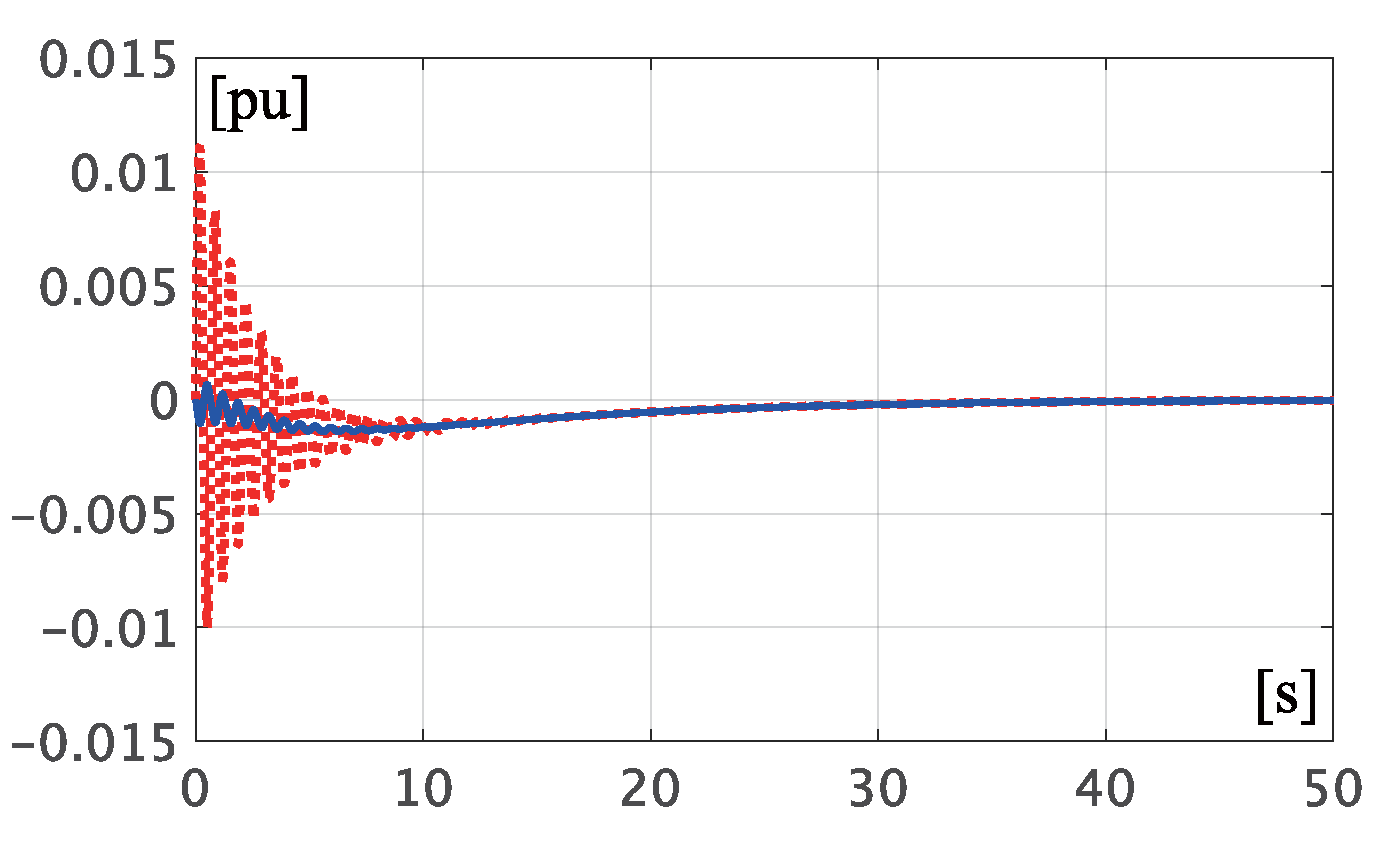
\includegraphics[width = 1.0\linewidth]{figs/P1ini}
    \subcaption{ \ref{table:pflow1}の定常潮流状態}
  \end{minipage}
  \begin{minipage}{0.49\linewidth}
    \centering
    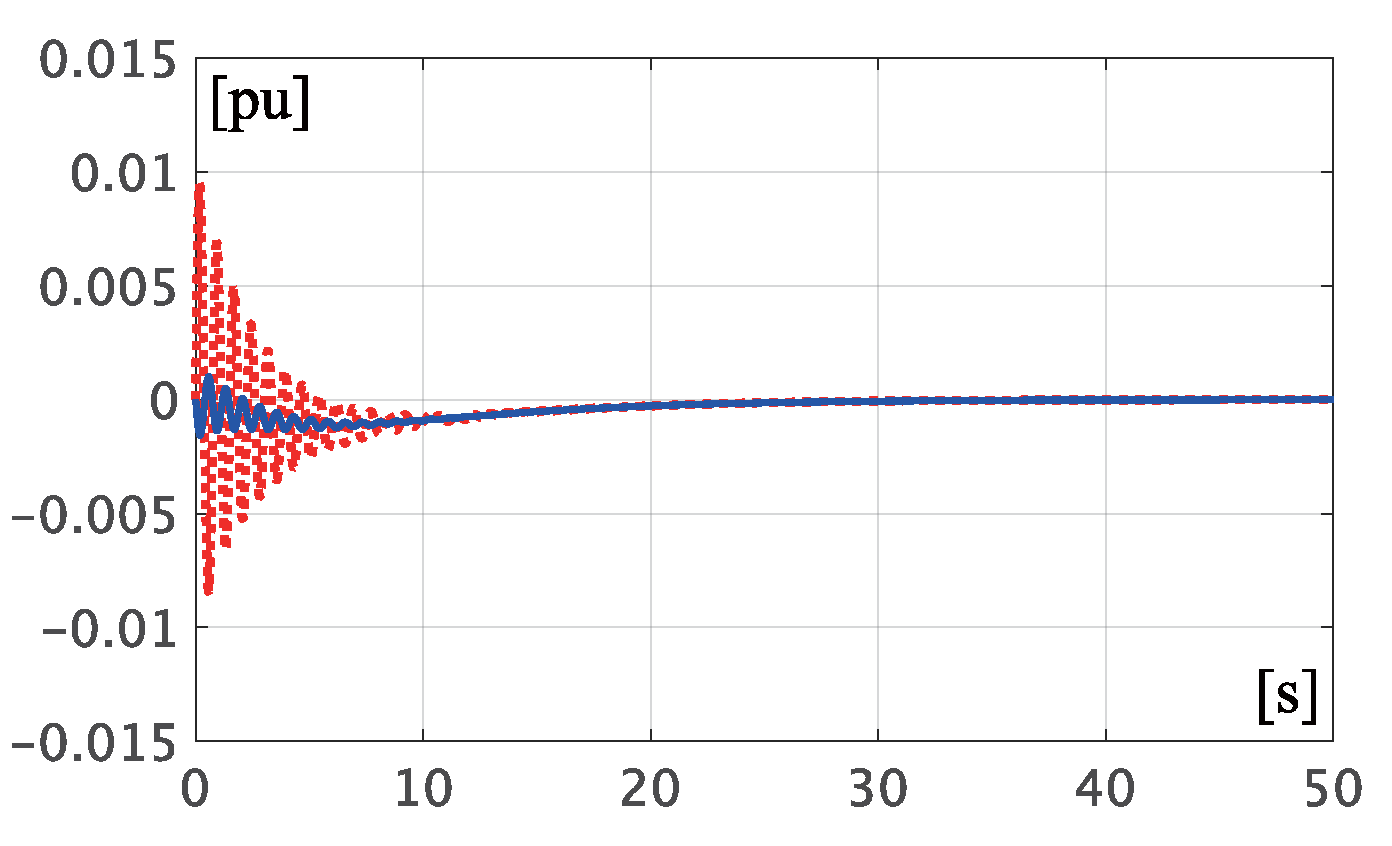
\includegraphics[width = 1.0\linewidth]{figs/P3ini}
    \subcaption{ \ref{table:pflow2}の定常潮流状態}
  \end{minipage}
  \medskip
  \caption{\textbf{初期値変動に対する角周波数偏差の時間応答}
  \\ \centering(青実線:$\Delta \omega_1$,赤破線:$\Delta \omega_3$)}
  \label{fig:P13ini}
  }
\medskip
\end{figure}

\subsection{負荷モデルのパラメータ変動に関する応答}\label{sec:resldpara}

定常潮流状態にある電力系統モデルに対して,負荷モデルの定数を1つでも変化させると,一般にすべての母線における電圧フェーザと電流フェーザの値が変化する。
このとき,一般に系統全体での電力の需給がバランスしなくなるため,与えられた界磁入力の値に応じて,機械入力の値を適切に修正しない限りは,各発電機の角周波数偏差は0に収束しない。
このことを確認してみよう。

\begin{例}[負荷のインピーダンス変化に対する電力系統モデルの時間応答]\label{ex:loadpv}
例\ref{ex:inires}と同じ設定で負荷のインピーダンス値が変化した場合の角周波数偏差の時間応答を計算してみよう。
具体的には,潮流計算の結果から逆算された負荷の抵抗を1\%増加または減少させて時間応答を計算する。
増加後と減少後の負荷のインピーダンス値は,\TABref{table:loadpara1}と\TABref{table:loadpara2}の2行目と3行目に示されている。

計算結果を\FIGref{fig:P1load}と\FIGref{fig:P3load}に示す。
青の実線は発電機1の角周波数偏差,赤の破線は発電機3の角周波数偏差を表している。
どの場合においても,2つの発電機の角周波数偏差が同期して変化していることがわかる。
また,抵抗が増加すると有効電力の消費が一般に大きくなるため,発電機の周波数は低下する。
抵抗が減少する場合は逆である。
発電機の機械入力が抵抗が変化する前の値で固定されているため,有効電力の需給バランスが取れなくなり,角周波数偏差の定常値は非零となっていることに注意されたい。
なお,負荷の抵抗の変化比率は\FIGref{fig:P1load}と\FIGref{fig:P3load}の両者で等しいが,生じる角周波数偏差の値は異なっている。
これは電力系統モデルの平衡点の選び方によって,外乱に対する感度(安定度)が変化することを示唆している。
\end{例}

\begin{figure}[t]
  \centering
  {
  \begin{minipage}{0.49\linewidth}
    \centering
    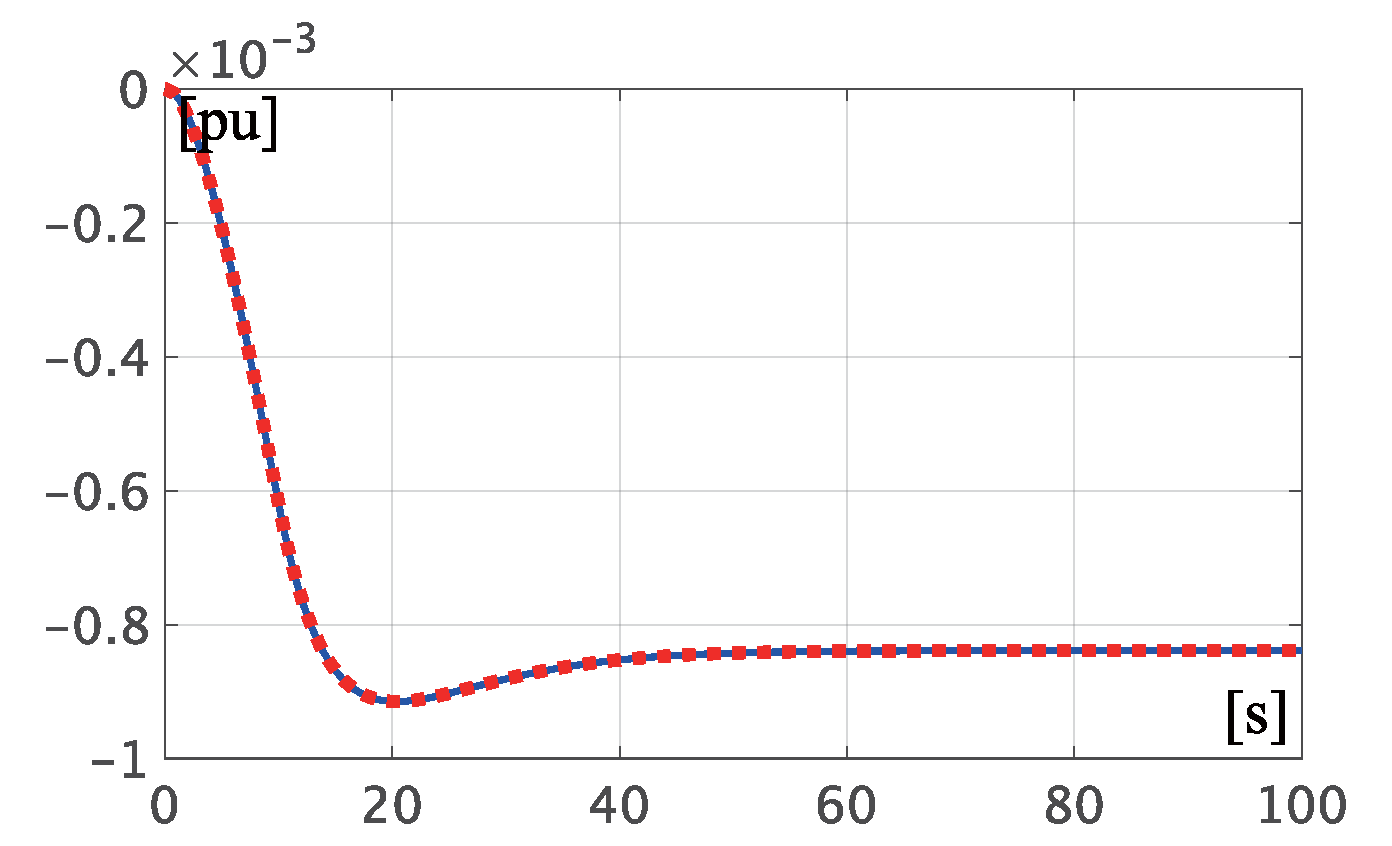
\includegraphics[width = 1.0\linewidth]{figs/P1mi}
    \subcaption{ 抵抗が1\%増加した場合 }
  \end{minipage}
  \begin{minipage}{0.49\linewidth}
    \centering
    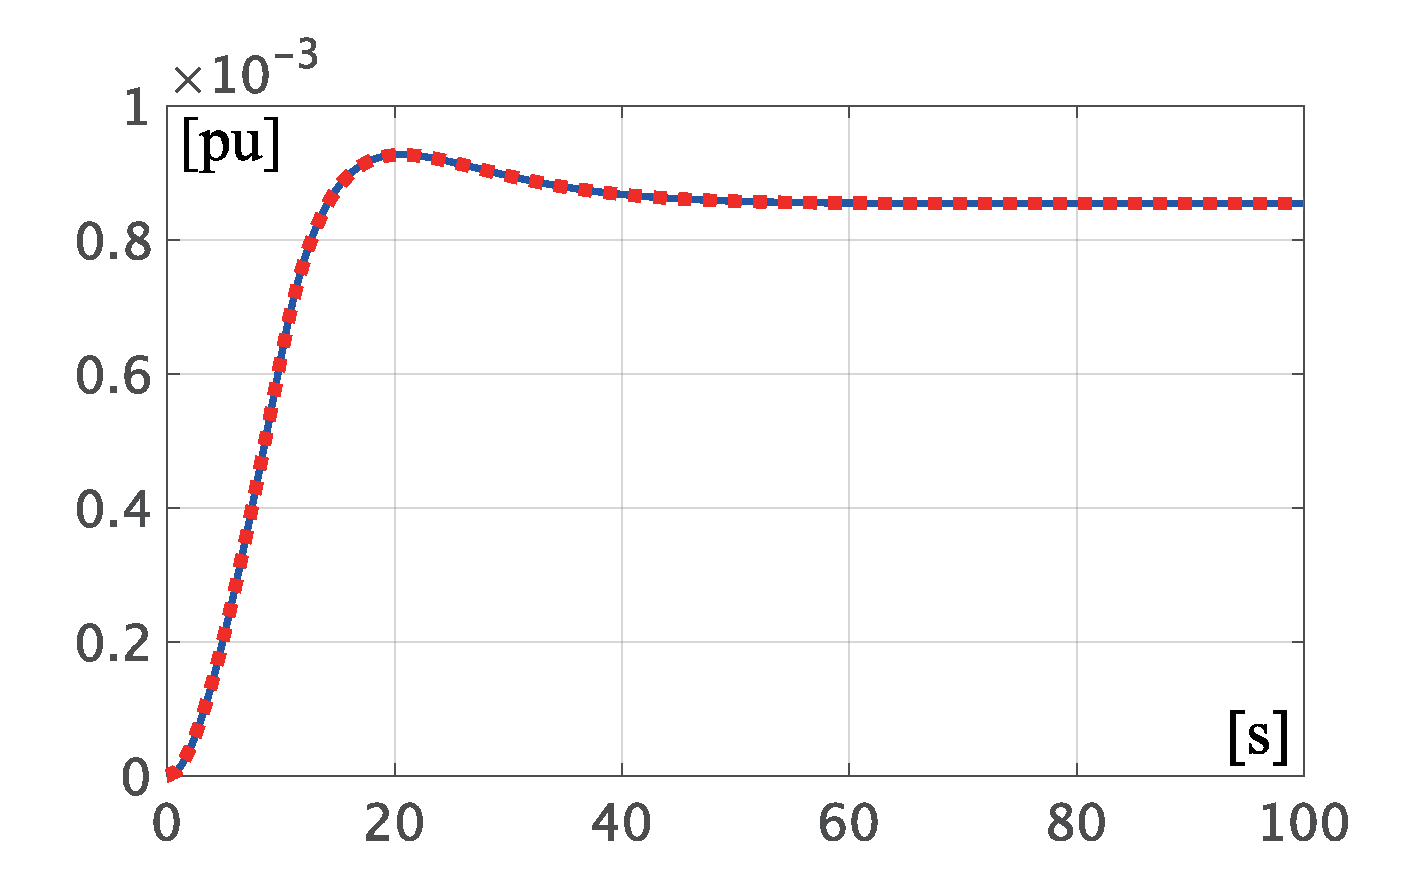
\includegraphics[width = 1.0\linewidth]{figs/P1pl}
    \subcaption{抵抗が1\%減少した場合 }
  \end{minipage}
  \medskip
  \caption{\textbf{負荷の変化に対する角周波数偏差の時間応答}
  \\ \centering(\ref{table:pflow1}の定常潮流状態,線種は\ref{fig:P13ini}と同様)}
  \label{fig:P1load}
  }
\medskip
\end{figure}

\begin{figure}[t]
  \centering
  {
  \begin{minipage}{0.49\linewidth}
    \centering
    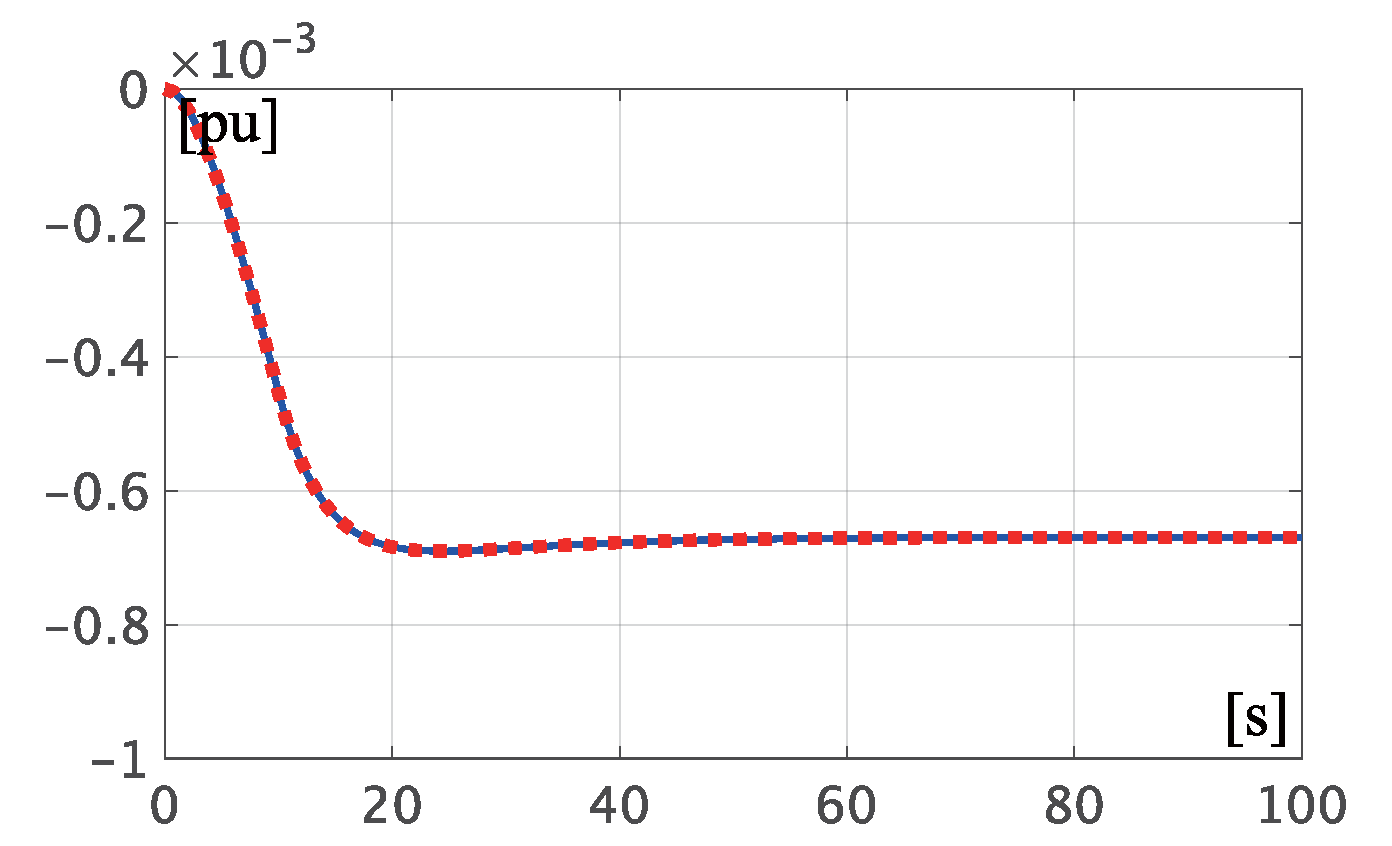
\includegraphics[width = 1.0\linewidth]{figs/P3mi}
    \subcaption{ 抵抗が1\%増加した場合 }
  \end{minipage}
  \begin{minipage}{0.49\linewidth}
    \centering
    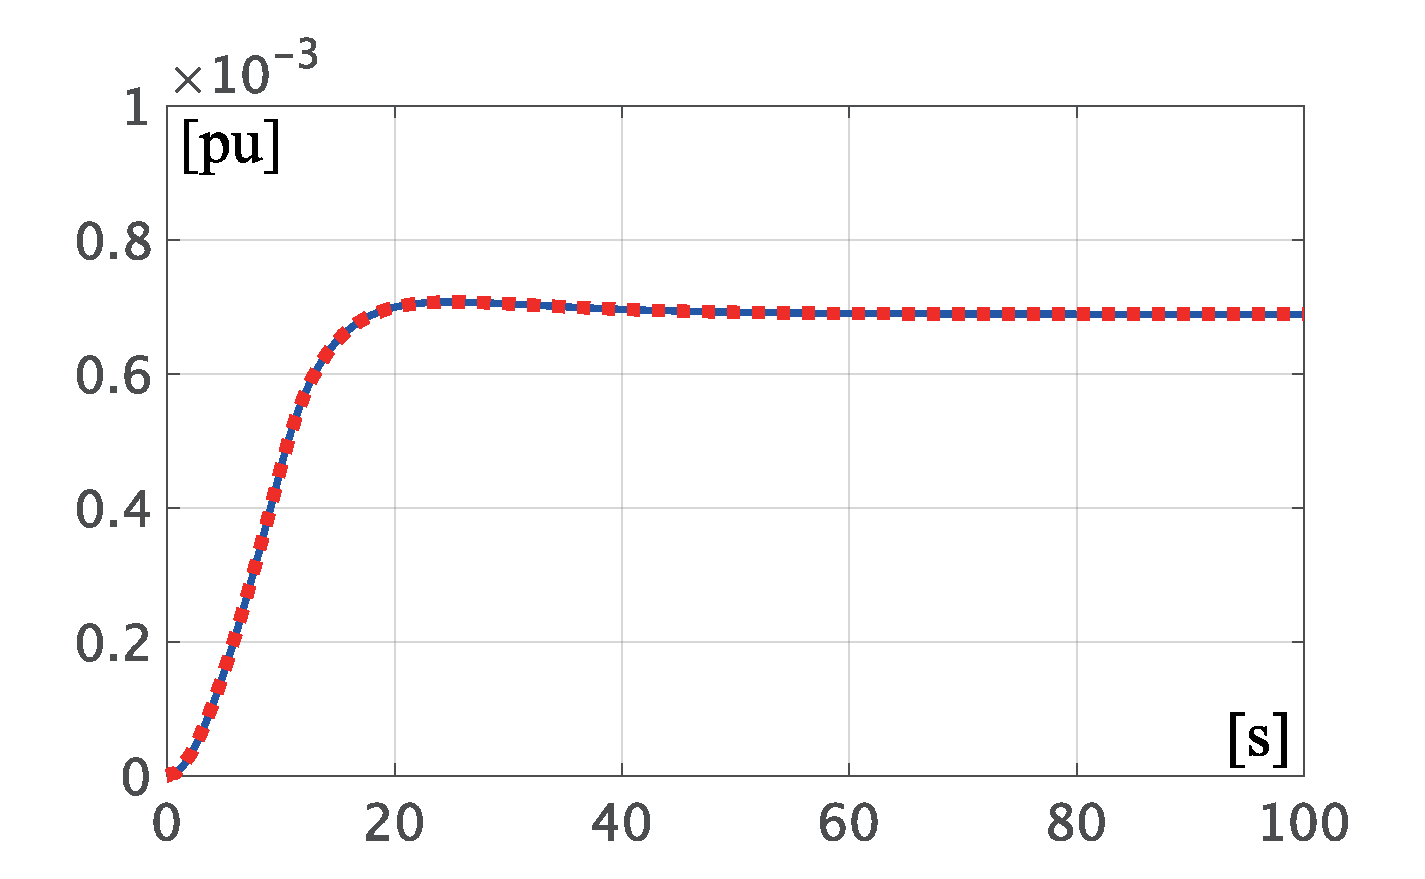
\includegraphics[width = 1.0\linewidth]{figs/P3pl}
    \subcaption{抵抗が1\%減少した場合 }
  \end{minipage}
  \medskip
  \caption{\textbf{負荷の変化に対する角周波数偏差の時間応答}
  \\ \centering(\ref{table:pflow2}の定常潮流状態,線種は\ref{fig:P13ini}と同様)}
  \label{fig:P3load}
  }
\medskip
\end{figure}

例\ref{ex:loadpv}では,例\ref{ex:inires}の結果とは異なり,発電機の角周波数偏差が非零の定常値をもつ。
この角周波数偏差を0にするためには,発電機群の機械入力もしくは界磁入力の値を適切に調整する必要がある。
これに対して,角周波数偏差の定常値を0にすることは,有効電力の需要と供給をバランスさせることであるため,発電機群の機械入力を調整する制御アルゴリズムにより周波数制御が行われることが一般的である。
ただし,すべての負荷の変化量を正確に計測することは現実的に困難である。
したがって,積分器に基づく制御動作により,需給バランスを達成する機械入力の値を自動探索するフィードバック制御が必要となる。
その詳細は,\ref{sec:agcover}節や\ref{sec:mathnpas}節で後述する。


\subsection{地絡による応答}\label{sec:fault}

\smallskip
\subsubsection{地絡とは}

物体と送電線の接触や落雷などをきっかけに電気回路が大地と接触して,大地に大きな電流が流れる現象は\textbf{地絡}(ground fault)\index{ ちらく@地絡}と呼ばれる。
地絡が長時間継続すると接続されている機器や設備などが損傷してしまうため,電力系統では地絡の発生を検知して地絡電流を遮断する装置が高速に作動する。
地絡電流を除去した後で遮断を解除すれば,地絡発生前の電力系統運用に復帰する。

地絡の発生を検知して地絡を除去するまでに要する時間は,概ね70~[ms]程度である。
この間に大地に流れる地絡電流が,電力系統の状態を大きく変動させるシビアな外乱となる。
なお,地絡による外乱は外部入力としてモデル化されるものではなく,「地絡が継続している時刻では別の電力系統モデルに切り替わる変動」としてモデル化される。

\smallskip
\subsubsection{母線地絡の定式化}

本書で扱う母線に発生する地絡は,地絡が継続している時刻において,その母線の電圧フェーザの値が0に拘束されるものとしてモデル化される。
以下では,$N$個の母線で構成される電力系統モデルに対して,一般性を失うことなく,母線$1$に地絡が発生するものとして説明する。
また,地絡は時刻0~[s]に発生し,時刻$t_0$~[s]まで継続するものとする。
このとき,式\ref{eq:pfconIV}の潮流状態は,$t<0$と$t\geq t_0$の時刻では,式\ref{eq:ohmY2}の平常時の代数方程式を満たすが,地絡が継続している$ t \in [0, t_0)$の時刻では,地絡母線の電流フェーザ$\bm{I}_{1}(t)$に関する方程式を除いた
\begin{subequations}\label{eq:ohmY2f}
 \begin{align}
\mat{
  \bm{I}_2(t)\\
  \vdots\\
  \bm{I}_{N}(t)
}
 =
\mat{
  \bm{Y}_{22} & \cdots & \bm{Y}_{2N}\\
  \vdots & \ddots & \vdots\\
  \bm{Y}_{N2} & \cdots & \bm{Y}_{NN}
}
\mat{
  \bm{V}_2(t)\\
  \vdots\\
  \bm{V}_{N}(t)
}
\end{align}
の代数方程式と,地絡母線の電圧フェーザに対する拘束条件
\begin{align}
|\bm{V}_{1}(t)| = 0
\end{align}
\end{subequations}
を満たさなければならない。
なお,地絡が発生していない母線や時刻では,電流フェーザと電圧フェーザは,各機器のモデルとして表される微分方程式または代数方程式にしたがう。
これは平常時と同じである。
すなわち,数値シミュレーションでは
\begin{itemize}
\item 地絡が発生していない時刻では,平常の電力系統モデル
\item 地絡が継続している時刻では,地絡が発生している母線とその母線に接続されている機器や送電線を取り除いた電力系統モデル
\end{itemize}
を切り替えて用いることに等しい。

地絡時に機器$1$から母線$1$に流入する電流フェーザ$\bm{I}_{1}(t)$は,機器の動特性から定められる。
具体的には,機器が発電機である場合には,$ t \in [0, t_0)$の時刻では,$|\bm{V}_{1}(t)|$を0とした
\begin{align}\label{eq:gendynVIfN}
\simode{
\dot{\delta}_1&= \omega_0  \Delta \omega_1\\
M_1   \Delta \dot{\omega}_1 &= 
 - D_1 \Delta\omega_1  
+P_{{\rm mech}1} 
\\
\taud_1 \dot{E}_1 & = 
- \tfrac{ \Xs_1 }{ \Xt_1 }E_1
+ V_{{\rm field}1}
}
\end{align}
の微分方程式にしたがって発電機の内部状態が時間発展する。
このとき,電流フェーザ$\bm{I}_{1}(t)$は,発電機の出力として
\begin{align*}%\label{eq:IoutfN}
|\bm{I}_1(t)|=\frac{E_1 (t)}{ \Xt_1 }
,\qquad
\angle \bm{I}_1 (t) = \delta_1 (t) - \frac{\pi}{2}
\end{align*}
で与えられる。
同様に,機器$1$が定インピーダンスの負荷モデルである場合には,式\ref{eq:cimp}の$|\bm{V}_{1}(t)|$が0であるため,$|\bm{I}_{1}(t)|$も0となる。
他の負荷モデルの場合も基本的に同様であるが,定電力の負荷モデルでは$|\bm{I}_{1}(t)|$が無限大となるため,数値シミュレーションでは数値的な不安定性に注意する必要がある。
なお,母線$1$から大地に流れる地絡電流フェーザは
\[
\bm{I}_{1}'(t) := \bm{I}_{1}(t) - \sum_{j=2}^{N} \bm{Y}_{1j} \bm{V}_{j}(t),\qquad
 t \in [0, t_0)
\]
と表すことができる。

地絡電流フェーザの値は,電力系統モデルの数値シミュレーションを実行する目的では計算する必要はない。
一方で,地絡母線に発電機が接続されている場合には,地絡が除去される時刻$t_0$における発電機の内部状態の値を計算することが重要であるため,式\ref{eq:gendynVIfN}の微分方程式は解く必要がある。
地絡が発生する時刻の電力系統モデルの内部状態,すなわち,初期時刻における各発電機の内部状態には,任意の潮流状態における値を設定すれば良い。
本書では,潮流計算の結果として求められた適当な定常潮流状態の値を設定する。
なお,地絡が発生する時刻や除去される時刻では,各発電機の内部状態は連続であるが,各母線の電圧フェーザや電流フェーザは不連続に変化する。

以上の母線地絡に対する時間応答の計算は,つぎの手順にまとめられる。

\medskip
\begin{breakbox}
\begin{itemize}
\item[(a)] 潮流計算で求められた定常潮流状態における変数値を各発電機の内部状態の初期値として設定する。
\item[(b)] 地絡が継続している$ t \in [0, t_0)$の時刻では,地絡が発生している母線とその母線に接続されている機器や送電線を取り除いた電力系統モデルによって時間発展を計算する。
\item[(c)] 地絡が発生している母線に発電機が接続されている場合には,地絡が継続している$ t \in [0, t_0)$の時刻では母線電圧フェーザを0に設定して,その発電機の内部状態の時間発展を計算する。
\item[(d)] 時刻$t_0$における各発電機の内部状態の値を設定して,すべての機器が接続された平常の電力系統モデルにより地絡除去後の時間発展を計算する。
\end{itemize}
\end{breakbox}
\medskip


この手順にしたがって母線地絡による時間応答を計算してみよう。

\begin{例}[母線地絡に対する電力系統モデルの時間応答]\label{ex:busflt}
例\ref{ex:inires}や例\ref{ex:loadpv}と同じ設定で,母線の地絡に対する角周波数偏差の時間応答を計算してみよう。
具体的には,電力系統が潮流計算で求められた2つの定常潮流状態を初期値に設定して,母線1に地絡が生じた場合の時間応答を計算する。
比較のため,地絡が除去されるまでの時間が50~[ms]である場合と,100~[ms]である場合の2通りを考える。

計算結果を\FIGref{fig:P1fault}と\FIGref{fig:P3fault}に示す。
青の実線は発電機1の角周波数偏差,赤の破線は発電機3の角周波数偏差を表している。
\FIGref{fig:P1fault}から,\TABref{table:pflow1}の定常潮流状態では,発電機3の周波数の振動が大きいことがわかる。
特に,地絡の継続時間が100~[ms]である場合にはより大きな振動が生じている。
発電機3の振動がより大きい理由は,\TABref{table:genparams}に示されているように,発電機1の慣性定数が100~[s]と大きいのに対して,発電機3の慣性定数は12~[s]と小さいためである。
すなわち,慣性が大きい発電機の振動が慣性が小さい発電機の大きな振動を引き起こしている。

一方で,\TABref{table:pflow2}の定常潮流状態では,同じ地絡に対しても周波数の振動が小さいことが\FIGref{fig:P3fault}からわかる。
この理由は,\ref{table:pflow1}の定常潮流状態では,小さな慣性をもつ発電機3から負荷で消費される有効電力の大半を供給していたのに対して,\ref{table:pflow2}の定常潮流状態では,大きな慣性をもつ発電機1から有効電力の大半を供給していたためである。
一般に,同期発電機は,供給する電力が最大に近づくほど外乱に対する感度も高くなる特性をもつ。
\ref{table:pflow2}の定常潮流状態では,慣性の小さい発電機3の安定度が相対的に高いため,地絡に対する角周波数偏差の感度が低くなっている。
\end{例}


\begin{figure}[t]
  \centering
  {
  \begin{minipage}{0.49\linewidth}
    \centering
    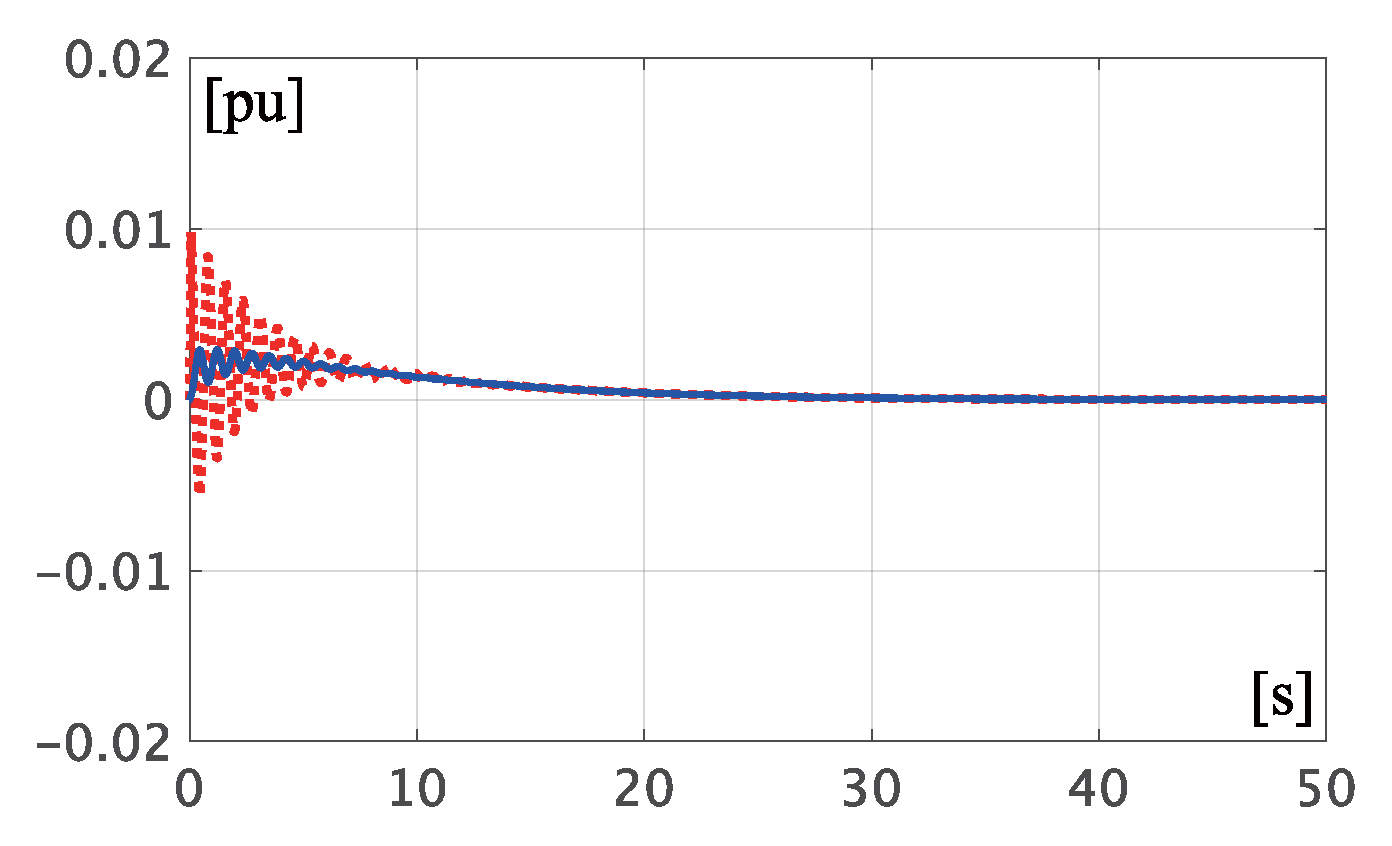
\includegraphics[width = 1.0\linewidth]{figs/50mP1}
    \subcaption{ 50~[ms]の地絡}
  \end{minipage}
  \begin{minipage}{0.49\linewidth}
    \centering
    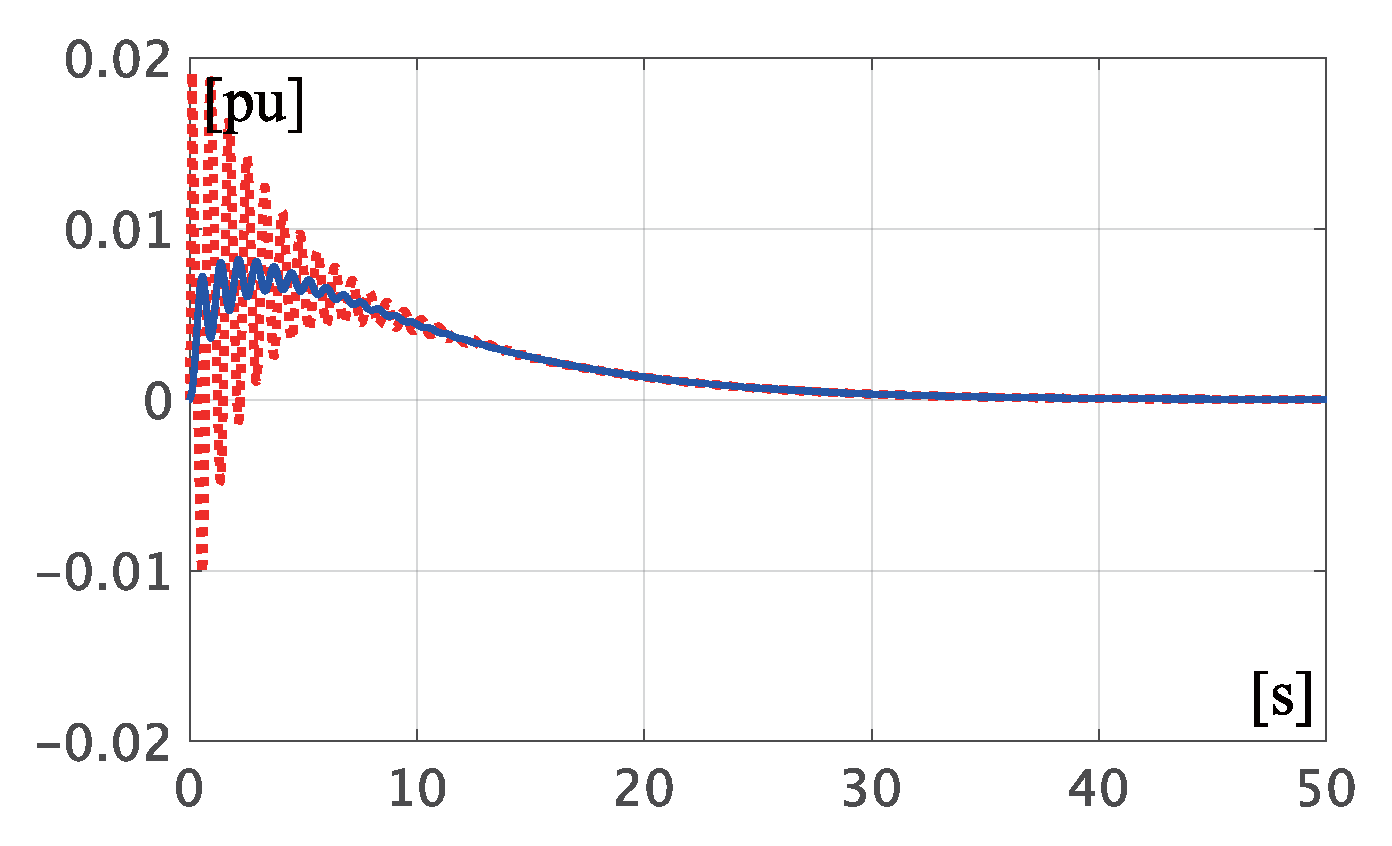
\includegraphics[width = 1.0\linewidth]{figs/100mP1}
    \subcaption{ 100~[ms]の地絡 }
  \end{minipage}
  \medskip
  \caption{\textbf{地絡に対する角周波数偏差の時間応答}
  \\ \centering (\ref{table:pflow1}の定常潮流状態,線種は\ref{fig:P13ini}と同様)}
  \label{fig:P1fault}
  }
\medskip
\end{figure}

\begin{figure}[t]
  \centering
  {
  \begin{minipage}{0.49\linewidth}
    \centering
    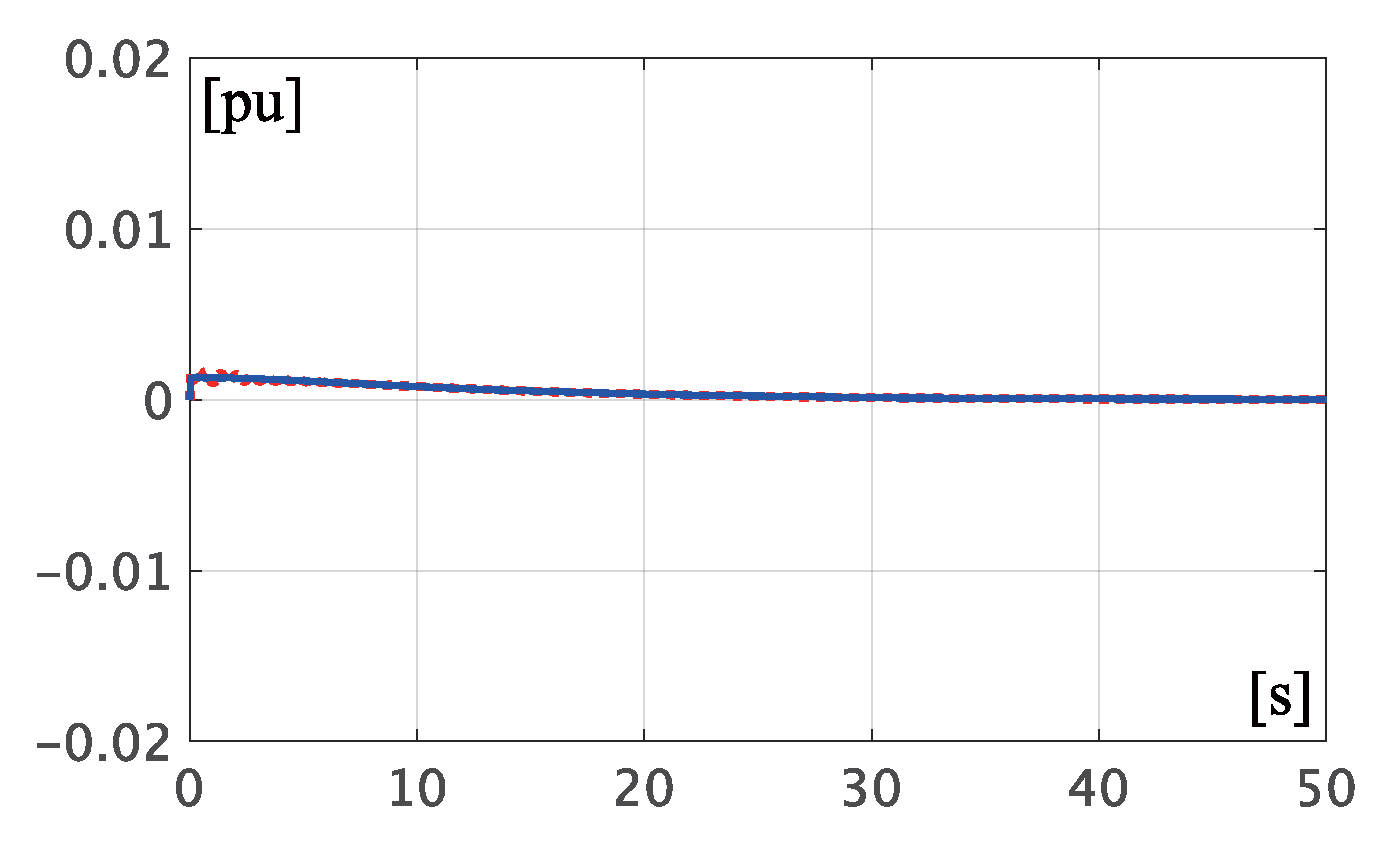
\includegraphics[width = 1.0\linewidth]{figs/50mP3}
    \subcaption{ 50~[ms]の地絡\label{fig:P3faulta}}
  \end{minipage}
  \begin{minipage}{0.49\linewidth}
    \centering
    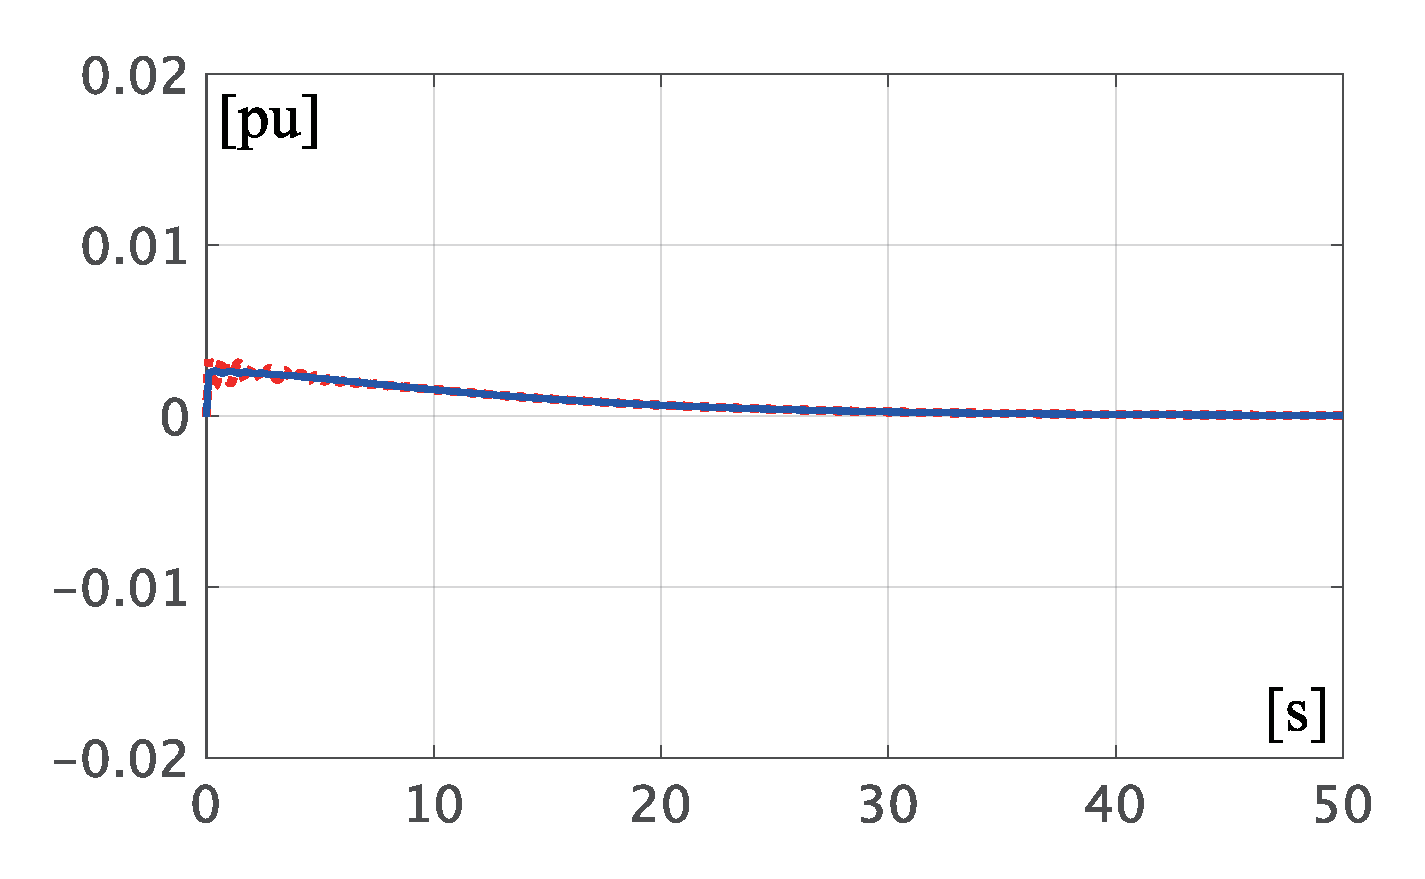
\includegraphics[width = 1.0\linewidth]{figs/100mP3}
    \subcaption{100~[ms]の地絡}
  \end{minipage}
  \medskip
  \caption{\textbf{地絡に対する角周波数偏差の時間応答}
  \\ \centering (\ref{table:pflow2}の定常潮流状態,線種は\ref{fig:P13ini}と同様)}
  \label{fig:P3fault}
  }
\medskip
\end{figure}

例\ref{ex:busflt}から,定常的な潮流状態(平衡点)に応じて,地絡に対する電力系統モデルの安定度が変化することがわかる。
特に,例\ref{ex:pf3bus}では,\TABref{table:pflow1}の定常潮流状態が送電損失の観点で優れていたのに対して,例\ref{ex:busflt}では,\TABref{table:pflow2}の定常潮流状態が地絡に対する系統安定度の観点で優れていることがわかる。
これらの例では,経済性や安定度などに関するトレードオフを考慮して,望ましい平衡点を探索することの重要性が示唆されている。
なお,地絡は特定の母線や送電線のみに発生するものではなく,様々な地点で発生する可能性があるため,電力系統全体の安定度を適切な意味で向上させる必要がある。
そのための制御機構は,\ref{sec:transcont}節や\ref{sec:retrofit}節で説明する。

なお,例\ref{ex:inires}から例\ref{ex:busflt}のシミュレーション結果から,内部状態が発散することなくある定常状態に落ち着いた場合には,「すべての発電機の角周波数偏差が同じ値に収束していること」がわかる。
同様の結果は,例\ref{ex:Kronode}でも観察されている。
定常潮流状態におけるこの周波数の同期は,電力系統モデルにおいて普遍的な現象である。
\ref{sec:agcover}節や\ref{sec:mathnpas}節で後述する周波数制御では,定常潮流状態で周波数が自動的に同期することを前提に制御アルゴリズムが構築される。

\section{定常的な潮流状態における母線電圧の同期\advanced}\label{sec:phsync}

本節では,\ref{sec:numsimtr}節で観察された周波数の同期現象を送電網のグラフ構造の観点から数学的に考察する。
定理\ref{thm:outst}の結果に基づき,つぎの定義を導入する。

\begin{定義}[定常潮流状態と母線電圧の同期]
\label{def:sync}
式\ref{eq:PQVgen}の連立方程式によって機器群が結合された電力系統モデルを考える。
すべての母線$i$に対して
\begin{align}\label{eq:stapfs}
\frac{dP_i}{dt}(t)=0
,\quad
\frac{dQ_i}{dt}(t)=0
,\quad
\frac{d|\bm{V}_i|}{dt}(t)=0
,\quad
\frac{d^2 \angle \bm{V}_i }{dt^2}(t)=0
\end{align}
がすべての$t\geq0$に対して成り立つとき,電力系統は\textbf{定常潮流状態}\index{ ていじょうちょうりゅうじょうたい@定常潮流状態}にあると呼ぶ
\footnote{
この「定常潮流状態」の数学的な定義は本書独自のものであり,電力系統工学で一般に用いられる定義ではないことに注意されたい。
}。
また,電力系統が定常潮流状態にあり,かつ
\begin{align}\label{eq:defsyn}
\frac{d \angle \bm{V}_i}{dt}(t) =  \frac{d \angle \bm{V}_j}{dt}(t)
\end{align}
が成り立つとき,定常潮流状態で母線$i$と母線$j$は\textbf{同期}\index{ どうき@同期}すると呼ぶ。
\end{定義}

定理\ref{thm:outst}に示されているように,発電機母線に対しては,式\ref{eq:stapfs}が成り立つことと,発電機の内部状態と外部入力が定常状態にあることは等価である。
また,任意に選ばれた母線の組$(i,j)$が定義\ref{def:sync}の意味で同期しているのであれば,すべての発電機の角周波数偏差が同じ値に収束することが結論づけられる。
なお,いずれの母線に対しても,式\ref{eq:stapfs}が成り立つことは,電流フェーザ$\bm{I}_i$に対して
\begin{align*}
\frac{d|\bm{I}_i|}{dt}(t)=0
,\qquad
\frac{d^2 \angle \bm{I}_i }{dt^2}(t)=0
,\qquad
\frac{d \angle \bm{I}_i }{dt}(t) = \frac{d \angle \bm{V}_i }{dt} (t)
\end{align*}
が成り立つことを意味する。
このことは
\begin{align*}
|P_i(t) + \bm{j} Q_i(t)| = |\bm{V}_i(t)| |\bm{I}_i(t)|
,\qquad
\angle(P_i(t) + \bm{j} Q_i(t)) = \angle \bm{V}_i(t) - \angle \bm{I}_i(t)
\end{align*}
であることから簡単に確認することができる。

母線$i$と送電線で結ばれている隣接母線の集合を$\mathcal{N}_i$と表す。
すなわち
\begin{align*}
\mathcal{N}_i:=
\left\{
j : \bm{Y}_{ij} \neq 0,\ \  j \neq i
\right\}
\end{align*}
であるものとする。
%母線$i$は,$\mathcal{N}_i$に含まないことに注意されたい。
母線$i$と送電線で結ばれている隣接母線の数は$|\mathcal{N}_i|$であり,このことを「母線$i$の\textbf{次数}(degree)\index{ degree@次数}は$|\mathcal{N}_i|$である」と呼ぶ。
また,電力系統モデルは定常潮流状態にあることを仮定して
\begin{align*}
\angle \bm{V}_i (t) = \Omega_i t +\phi_i
\end{align*}
と表す。
ただし,$\Omega_i$と$\phi_i$は定数である。
このとき,式\ref{eq:PQVgen}の母線$i$に関する電力バランス方程式は
\[
P_i + \bm{j} Q_i = \sum_{j=1}^N \overline{\bm{Y}}_{ij} |\bm{V}_i| |\bm{V}_j|
e^{\bm{j} \left\{ ( \Omega_i - \Omega_j )t + \phi_i -\phi_j \right\}}
\]
となる。
ここで,定常潮流状態を仮定する場合には,母線$i$に供給される有効電力と無効電力,母線電圧フェーザの絶対値はすべて定数であり,それらを$P_i^{\star}$,$Q_i^{\star}$,$|\bm{V}_i^{\star}|$と表せば,この電力バランス方程式は
\begin{align}\label{eq:sumcirc}
\underbrace{
\frac{1}{|\mathcal{N}_i|}\sum_{j \in \mathcal{N}_i } 
r_{ij}
e^{\bm{j} 
\left(
\Omega_{ij}t + 
\Phi_{ij}
\right) }
}_{\bm{C}_i (t)}
= \bm{z}_i
\end{align}
と変形できる。
ただし,母線$i$と$j$の電圧フェーザの周波数差を
\[
\Omega_{ij}:=\Omega_{i}-\Omega_{j}
\]
と表している。
また,$r_{ij}$,$\Phi_{ij}$,$\bm{z}_i$はすべて定数であり
\begin{align*}
r_{ij} &:=|\bm{V}_i^{\star}| |\bm{V}_j^{\star}| |\bm{Y}_{ij}|, \\
\Phi_{ij} &:= \phi_i - \phi_j - \angle \bm{Y}_{ij},
\\
\bm{z}_i &:=  \tfrac{
\left\{
P_i^{\star} - \real[\bm{Y}_{ii}] |\bm{V}_i^{\star}|^2
+ \bm{j}
\left(
Q_i^{\star} + \imag [\bm{Y}_{ii}] |\bm{V}_i^{\star}|^2
\right)
\right\}
}
{|\mathcal{N}_i|}
\end{align*}
で定義される。

以下では,式\ref{eq:sumcirc}の方程式から,隣接する母線との同期を表す等式として,すべての$j\in \mathcal{N}_i$に対して$\Omega_{ij}$が0であること,すなわち
\begin{align}\label{eq:alloms}
\Omega_i = \Omega_{j} 
,\qquad 
\forall j\in \mathcal{N}_i
\end{align}
を導くことを考える。
ここで,式\ref{eq:sumcirc}は「原点を中心とする半径$r_{ij}$の円周上を,初期位相$\Phi_{ij}$,角速度$\Omega_{ij}$で等速運動する$|\mathcal{N}_i|$個の点の重心$\bm{C}_i (t)$が,複素平面上のある点$\bm{z}_i$で不変であること」を表している。
\FIGref{fig:centerg}には,母線$1$が母線$2$と母線$3$に接続している場合の関係を例示している。
この事実に注目するとつぎの結果が導ける。


\begin{figure}[t]
\centering
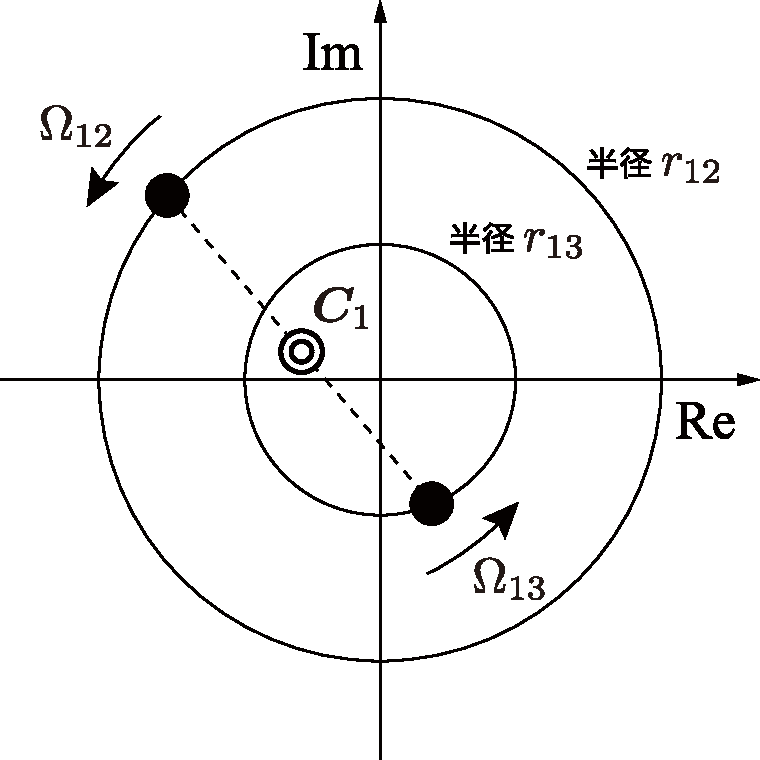
\includegraphics[width = .4\linewidth]{figs/centerg}
\medskip
\caption{\textbf{母線1が母線2と母線3に接続している場合}}
\label{fig:centerg}
\medskip
\end{figure}


\begin{補題}[電力潮流方程式から導かれる母線の同期]
\label{lem:sumc2}
実定数$r_{ij}$,$\Omega_i$,$\Omega_j$,$\Phi_{ij}$に対して,式\ref{eq:sumcirc}の$\bm{C}_i (t)$を考える。
ただし,$r_{ij}>0$とする。
このとき,$|\mathcal{N}_i|=1$であるならば,$\bm{C}_i (t)$が$t$に依らない定数であることは,式\ref{eq:alloms}と等価である。
また,$|\mathcal{N}_i|=2$であるならば,$\bm{C}_i (t)$が$t$に依らない定数であることは,式\ref{eq:alloms}
が成り立つこと,または
\begin{align}\label{eq:N2sing}
\Omega_{j_1} = \Omega_{j_2}
,\qquad
r_{i j_1} = r_{i j_2}
,\qquad
|\Phi_{i j_1}-\Phi_{i j_2}| = \pi
\end{align}
と等価である。
ただし,$\mathcal{N}_i = \{j_1,j_2\}$である。
さらに,$|\mathcal{N}_i|=3$であるならば,$\bm{C}_i (t)$が$t$に依らない定数であることは,式\ref{eq:alloms}が成り立つこと,または,$ \mathcal{N}_i =\{j_1,j_2,j_3\}$に対して
\begin{align}\label{eq:threeoms}
\Omega_{j_1} = \Omega_{j_2}= \Omega_{j_2}
,\qquad 
\sum_{j\in \mathcal{N}_i} 
r_{ij} e^{\bm{j} \Phi_{ij}}=0
\end{align}
が成り立つこと,
または,$\Omega_{i} = \Omega_{j_3}$を満たす$j_3 \in \mathcal{N}_i$に対して,式\ref{eq:N2sing}が成り立つことと等価である。
ただし,$ \mathcal{N}_i \setminus \{j_3\}=\{j_1,j_2\}$である。
\end{補題}

\begin{証明}
章末の補題\ref{lem:sumc}
を適用することで,$|\mathcal{N}_i|=1$と$|\mathcal{N}_i|=2$の場合の事実を示すことができる。
したがって,以下では$|\mathcal{N}_i|=3$の場合について考える。
表記の簡単化のため,$j \in\{1,2,3\}$とし,$r_{ij}$,$\Phi_{ij}$,$\Omega_i$,$\bm{C}_i$をそれぞれ$r_{j}$,$\Phi_{j}$,$\Omega_0$,$\bm{C}_0$と表す。
まず
\begin{align}\label{eq:omjeq}
\Omega_j \neq \Omega_0
,\qquad \forall j \in \{1,2,3\}
\end{align}
である場合を考える。
補題\ref{lem:sumc}から,式\ref{eq:omjeq}が成り立つとき,式\ref{eq:sumcirc}は
\begin{align*}
\Omega_1 = \Omega_2 = \Omega_3,\qquad
\sum_{j=1}^3 
r_j e^{\bm{j} \Phi_j}=0
\end{align*}
と等価であることがわかる。
これは式\ref{eq:threeoms}を意味している。
%しかしながら,$\Omega_1 = \Omega_2 = \Omega_3$である場合には,$|\mathcal{N}_i|=1$のときと同様にして,$\bm{C}_i (t)$が$t$に依らない定数であることと式\ref{eq:alloms}が等価であることが導かれる。
%これは式\ref{eq:omjeq}に矛盾する。

つぎに,式\ref{eq:omjeq}が成り立たない場合,すなわち,ある$j\in\{1,2,3\}$に対して$\Omega_0=\Omega_j$である場合を考える。
特に,$j$に関する対称性から,一般性を失うことなく,$\Omega_0=\Omega_3$である場合を考える。
このとき
\begin{align*}
\bm{C}_0 (t) = \frac{1}{3} \left\{
r_3 e^{\bm{j} \Phi_3}
+
\sum_{j=1}^2
r_{j}
e^{\bm{j} 
\left\{
(\Omega_0 - \Omega_j)t + 
\Phi_{j}
\right\} }
\right\}
\end{align*}
であることから,$t$に関する不変性は,$|\mathcal{N}_i|=2$の場合と同様に議論できる。
したがって,$\bm{C}_0 (t)$が$t$に依らない定数であることは,式\ref{eq:alloms}または
\begin{align*}
\Omega_{1} = \Omega_{2}
,\qquad
r_{1} = r_{2}
,\qquad
|\Phi_{1}-\Phi_{2}| = \pi
\end{align*}
と等価である。
以上より題意が示される。
\end{証明}

補題\ref{lem:sumc2}は,注目する母線の次数が1のとき,すなわち,\FIGref{fig:bussync}(a)のような端点の母線については,その母線と隣の母線が同期することを示している。
また,注目する母線(太線で示されたノード)の次数が2のとき,すなわち,\FIGref{fig:bussync}(b)のような鎖状経路にある母線については,少なくともその両隣の母線が同期する。
さらに,注目する母線の次数が3のとき,すなわち,\FIGref{fig:bussync}(c)のような3本の送電線で結ばれている節の母線については,注目する母線を除く3つが同期する,または,隣接する母線のうち少なくとも1つが注目する母線と同期する。
これは,隣接する母線の1つだけが同期しないような状況や,どの母線の組も同期しないような状況は生じないことも意味している。

\begin{figure}[t]
  \centering
  {
  \begin{minipage}{0.24\linewidth}
    \centering
    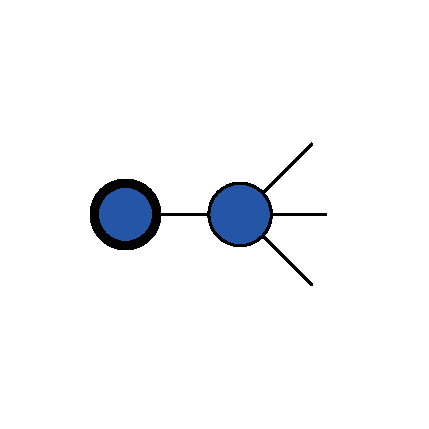
\includegraphics[width = .85\linewidth]{figs/1degbus}
    \subcaption{ 次数1の母線}
    \label{fig:N1} 
  \end{minipage}
  \begin{minipage}{0.24\linewidth}
    \centering
    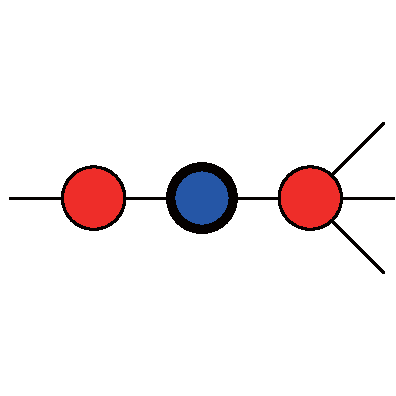
\includegraphics[width = .85\linewidth]{figs/2degbus}
    \subcaption{ 次数2の母線}
  \end{minipage}
  \label{fig:N2}
  \begin{minipage}{0.48\linewidth}
    \centering
    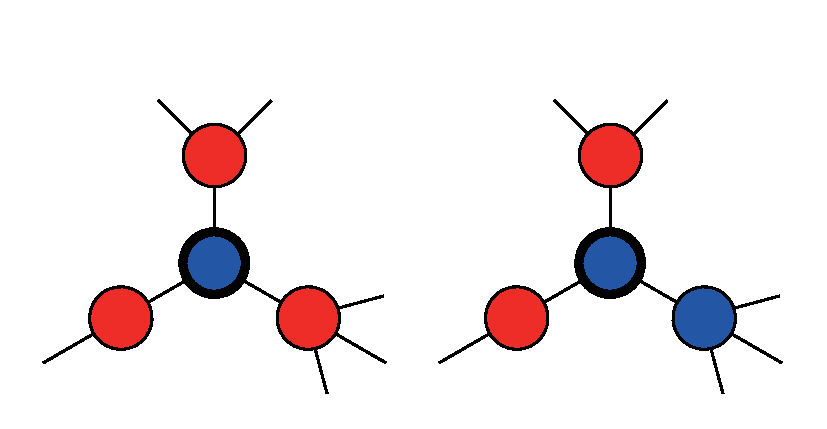
\includegraphics[width = .85\linewidth]{figs/3degbus}
    \subcaption{ 次数3の母線 }
  \end{minipage}
  \medskip
  \caption{\textbf{母線の次数に応じた隣接母線との同期}}
  \label{fig:bussync}
  }
\medskip
\end{figure}
注目する母線の次数が4以上である場合にも同様の解析を行うことは可能である。
しかしながら,得られる条件が$\Omega_i$や$\Omega_j$に関する高次の方程式になることや,任意に選ばれた一部の隣接母線のみが同期する場合などの複数の組み合わせが存在するため,同期に関する等価条件を書き下すことは一般に煩雑となる。
ただし,注目する母線$i$とそれに隣接する$|\mathcal{N}_i|$個の母線に対して,いずれかの$|\mathcal{N}_i |-1$個の隣接母線が母線$i$と同期するのであれば,残り1個の隣接母線も同期することは一般に示される。

補題\ref{lem:sumc2}で示されている次数が3以下の条件を組み合わせて用いることによって,次数が4以上の母線が送電網に含まれている場合にも,すべての母線の同期が示される場合は存在する。
例えば,連結であり閉路をもたない\textbf{木}(tree)\index{ き@木}の構造をもつ送電網に対して,つぎの事実を示すことができる。

\begin{定理}[木構造の送電網における母線の同期]
\label{thm:tree}
式\ref{eq:PQVgen}の連立方程式によって機器群が結合された電力系統モデルを考える。
送電網のグラフが木構造をもつとき,
%\footnote{
%グラフ理論において,連結であり閉路をもたないグラフは\textbf{木}(tree)と呼ばれる。
%},
定常潮流状態においてすべての母線は同期する。
\end{定理}

\begin{証明}
\FIGref{fig:treepr}(a)の太線で示された端点の母線に注目する。
母線の次数は1であるから,その隣の母線は端点の母線と同期する。
つぎに,端点の隣の母線が鎖状経路にある場合には,その母線の次数は2であるため,少なくともその両隣の母線は同期する。
これを繰り返していくことで,\FIGref{fig:treepr}(a)のように,端点と次数が3以上の節の母線を結ぶ鎖状経路において,すべての母線の同期が示される。

同様に,別の端点から次数が3以上の節に存在するすべての母線は同期するため,\FIGref{fig:treepr}のように,太線で示される節の母線に連結するすべての鎖状経路の母線はすべて同期することがわかる。
この議論を繰り返せば,木を構成するすべての母線が同期することが示される。
\end{証明}


\begin{figure}[t]
  \centering
  {
  \begin{minipage}{0.40\linewidth}
    \centering
    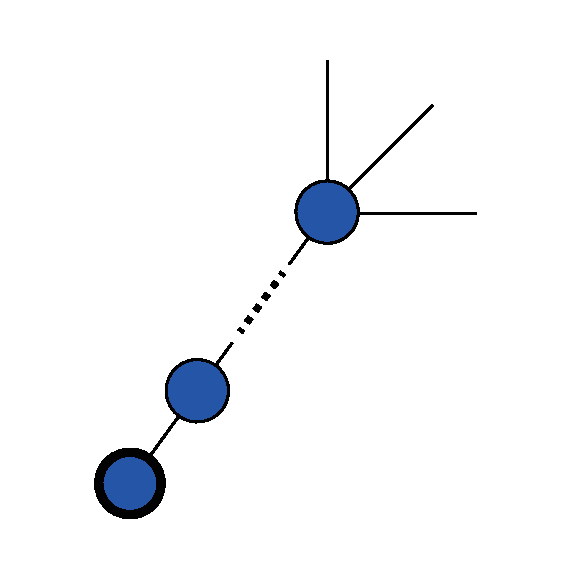
\includegraphics[width = .50\linewidth]{figs/treesub}
    \subcaption{ }
  \end{minipage}
  \begin{minipage}{0.40\linewidth}
    \centering
    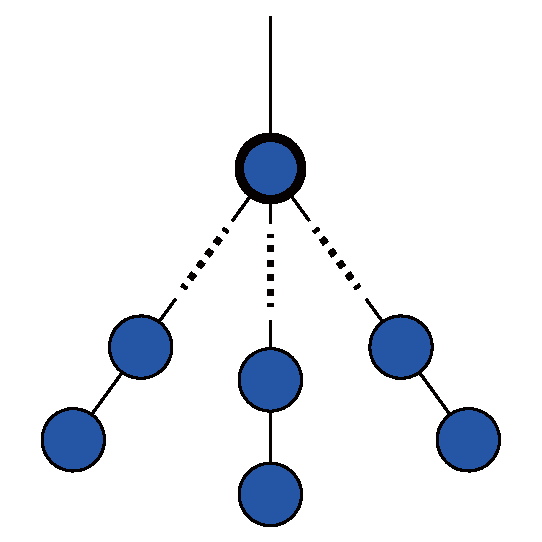
\includegraphics[width = .50\linewidth]{figs/tree}
    \subcaption{ }
  \end{minipage}
  \medskip
  \caption{\textbf{木構造をもつ送電網における母線の同期}}
  \label{fig:treepr}
  }
\medskip
\end{figure}
%\begin{figure}[t]
%\centering
%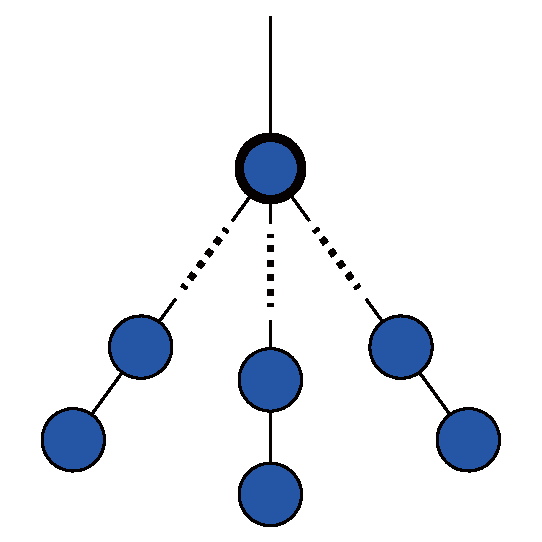
\includegraphics[width = .20\linewidth]{figs/tree}
%\caption{...}
%\label{fig:treepr}
%\medskip
%\end{figure}
定理\ref{thm:tree}に示されている木構造をもつ送電網の母線には次数の制限はない。
このように,仮に次数が4以上の母線が送電網に含まれていたとしても,グラフ構造の情報だけを用いて,すべての母線の同期を演繹できる場合がある。
同様に,つぎの事実を示すことができる。

\begin{定理}[円環構造の送電網における母線の同期]
\label{thm:circ}
式\ref{eq:PQVgen}の連立方程式によって機器群が結合された電力系統モデルを考える。
送電網のグラフが円環構造をもち,かつ,母線の総数が奇数であるとき,定常潮流状態においてすべての母線は同期する。
\end{定理}

\begin{証明}
ある母線に注目するとその両端の母線の同期が示される。
これを繰り返すことにより,母線の総数が奇数である場合にすべての母線の同期が示される。
\end{証明}

%\begin{figure}[t]
%  \centering
%  {
%  \begin{minipage}{0.3\linewidth}
%    \centering
%    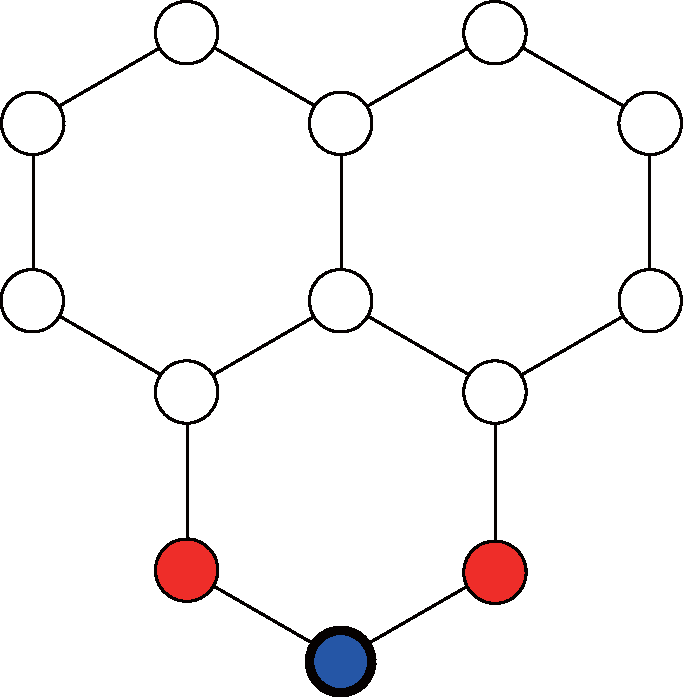
\includegraphics[width = .70\linewidth]{figs/honya}
%    \subcaption{  }
%  \end{minipage}
%  \begin{minipage}{0.3\linewidth}
%    \centering
%    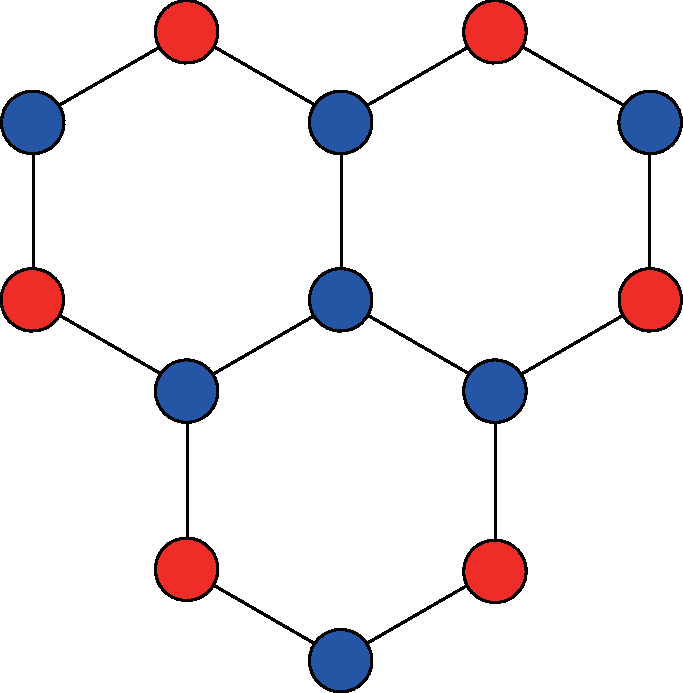
\includegraphics[width = .70\linewidth]{figs/honyb}
%    \subcaption{  }
%  \end{minipage}
%  \begin{minipage}{0.3\linewidth}
%    \centering
%    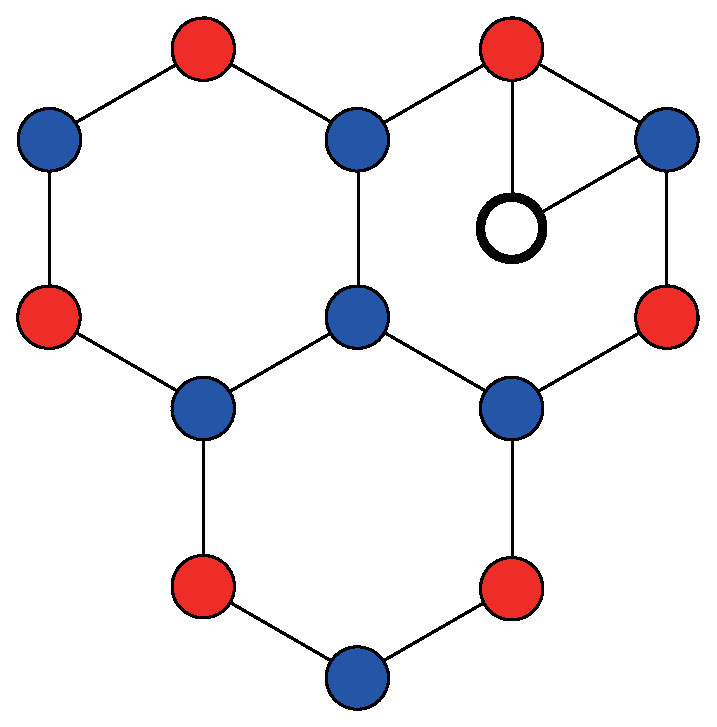
\includegraphics[width = .70\linewidth]{figs/honyc}
%    \subcaption{  }
%  \end{minipage}
%  \medskip
%  \caption{\textbf{ハニカム構造をもつ送電網における母線の同期}}
%  \label{fig:hony}
%  }
%\medskip
%\end{figure}

定理\ref{thm:circ}は,円環構造の送電網に対して,母線の総数が奇数である場合は,各送電網のアドミタンスの値などに依らず,すべての母線が同期することを示している。
一方で,母線の総数が偶数である場合には,送電線のアドミタンス値などの追加の情報を用いない限りは,円環構造の送電網に対してもすべての母線の同期を結論づけることはできない。

つぎの例では,母線の総数が偶数である場合にも,アドミタンスの値などの一部の情報が与えられるだけで,すべての母線の同期が示され得ることを示す。

%次数3の母線を含む送電網に補題\ref{lem:sumc2}を適用した例としてつぎを示す。

%\begin{例}[ハニカム構造の送電網における母線の同期]\label{ex:deg3}
%\FIGref{fig:hony}(a)に示されるハニカム構造をもつ送電網に対して,定常潮流状態における母線の同期を考えよう。
%最下部の母線に注目すると,その両隣の母線の同期がわかる。
%これらの同期する母線を赤で示し,最下部の母線と同期するものを青で示す。
%このとき,補題\ref{lem:sumc2}を各母線に適用していくことによって,同期するすべての母線群を\FIGref{fig:hony}(b)のように色分けすることができる。
%しかしながら,この場合には,グラフ構造の情報だけで赤の母線群と青の母線群の同期を結論づけることはできない。
%一方で,\FIGref{fig:hony}(c)のように母線が1つ追加された送電網の場合には,その追加された母線に注目することで,両隣の赤と青の母線の同期が導かれる。
%したがって,\FIGref{fig:hony}(c)のグラフ構造の場合には,すべての母線の同期が示される。
%\end{例}
%
%例\ref{ex:deg3}において,一部のグラフ構造の差異により同期する母線の対称性が崩れることで,電力系統全体での母線の同期が演繹されている点は興味深い。
%つぎの例では,アドミタンスの値まで考慮した「定量的な送電網の対称性」の観点から母線の同期を考察する。

\begin{figure}[t]
\centering
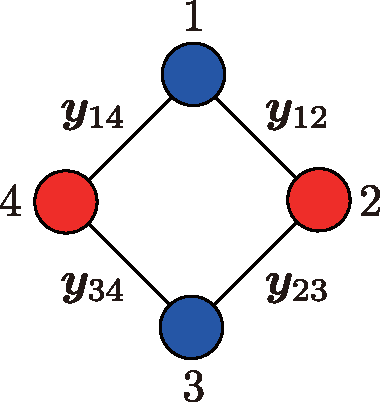
\includegraphics[width = .20\linewidth]{figs/4busbox}
\medskip
\caption{\textbf{円環構造をもつ送電網における4母線の同期}}
\label{fig:4busbox}
\medskip
\end{figure}

\begin{例}[円環構造の送電網における4つの母線の同期]\label{ex:symbox}
\FIGref{fig:4busbox}に示される円環構造をもつ送電網に対して,定常潮流状態における母線の同期を考えよう。
母線の数は偶数であるため,定理\ref{thm:circ}のようにグラフ構造の情報だけですべての母線の同期を示すことはできない。
ただし,\FIGref{fig:4busbox}の赤と青で示されているように,少なくとも互い違いの母線がそれぞれ同期することは補題\ref{lem:sumc2}からわかる。
したがって,すべての母線の同期を示すためには,少なくとも1つの母線に対して式\ref{eq:N2sing}のいずれかの条件が満たされないことを示せば良い。

母線$i$と母線$j$を結ぶ送電線のアドミタンスを$\bm{y}_{ij}$と表す。
このとき,各母線に対する式\ref{eq:N2sing}中央の条件は
\begin{align*}
|\bm{V}_2^{\star}||\bm{y}_{12}|&=|\bm{V}_4^{\star}||\bm{y}_{14}|
,\qquad
|\bm{V}_1^{\star}||\bm{y}_{12}|=|\bm{V}_3^{\star}||\bm{y}_{23}|,
\\
|\bm{V}_2^{\star}||\bm{y}_{23}|&=|\bm{V}_4^{\star}||\bm{y}_{34}|
,\qquad
|\bm{V}_3^{\star}||\bm{y}_{34}|=|\bm{V}_1^{\star}||\bm{y}_{14}|
\end{align*}
と書き下すことができる。
これを行列形式で表現すれば
\begin{align*}
\underbrace{
\mat{
0 & |\bm{y}_{12}| &  0  & -|\bm{y}_{14}|\\
-|\bm{y}_{12}| & 0 & |\bm{y}_{23}| & 0\\
0 & -|\bm{y}_{23}| & 0 & |\bm{y}_{34}|\\
|\bm{y}_{14}| & 0 & -|\bm{y}_{34}| & 0
}}_{S}
\mat{
|\bm{V}_1^{\star}|\\
|\bm{V}_2^{\star}|\\
|\bm{V}_3^{\star}|\\
|\bm{V}_4^{\star}|
}=0
\end{align*}
となる。
この方程式を満たす正のベクトル$(|\bm{V}_1^{\star}|,\ldots,|\bm{V}_4^{\star}|)$が存在するための必要条件は,左辺の$S$が正則でないことである。
%ただし,$S$が正則でない場合にも,正のベクトルがその零空間として存在するとは限らないことに注意されたい。
ここで,列ベクトルの疎構造から,$S$が非正則であるためには
\begin{align}\label{eq:ycond}
|\bm{y}_{12}||\bm{y}_{34}| = |\bm{y}_{14}||\bm{y}_{23}|
\end{align}
でなければならない。
したがって,アドミタンス行列がこの条件を満たさない限り,すべての母線は同期する。
なお,式\ref{eq:ycond}が満たされる場合には,所望の電圧フェーザの絶対値を定めることができるため,式\ref{eq:N2sing}中央の条件を満たす$(|\bm{V}_1^{\star}|,\ldots,|\bm{V}_4^{\star}|)$が存在するための必要十分条件が,式\ref{eq:ycond}であることも示される。

つぎに,式\ref{eq:N2sing}右の条件は,母線1と母線3に注目すれば
\begin{align*}
|\phi_2 - \phi_4 + \angle \bm{y}_{12} - \angle \bm{y}_{14}|=\pi
,\qquad
|\phi_2 - \phi_4 + \angle \bm{y}_{23} - \angle \bm{y}_{34}|=\pi
\end{align*}
と書き下すことができる。
同様に,母線2と母線4に注目すれば
\begin{align*}
|\phi_1 - \phi_3 + \angle \bm{y}_{12} - \angle \bm{y}_{23}|=\pi
,\qquad
|\phi_1 - \phi_3 + \angle \bm{y}_{14} - \angle \bm{y}_{34}|=\pi
\end{align*}
が得られる。
一般に,対地静電容量が十分に小さいとき,アドミタンスの実部であるコンダクタンス成分は非負であり,虚部であるサセプタンス成分は負であること,すなわち
\[
\angle \bm{y}_{ij} \in \left[-\frac{\pi}{2},0 \right)
\]
であることに注意すると,以上の条件を満たす$(\phi_1,\ldots,\phi_4)$が存在するための必要十分条件が
\begin{align}\label{eq:ycona}
\angle \bm{y}_{12} - \angle \bm{y}_{14}=
\angle \bm{y}_{23} - \angle \bm{y}_{34}
\end{align}
であることが導ける。
したがって,アドミタンス行列がこの条件を満たさない限り,すべての母線は同期する。

以上の議論から,定常潮流状態において同期しない母線の組が1つ以上存在するための必要十分条件は,式\ref{eq:ycond}かつ式\ref{eq:ycona}であることがわかる。
この2つの条件は,\FIGref{fig:4busbox}の送電網がアドミタンスの値に関する特異的な対称性をもつときにのみ,互い違いの母線のみが同期するような状況が起こることを示唆している。
\end{例}

例\ref{ex:symbox}から,式\ref{eq:N2sing}の条件は送電網のアドミタンスの値に関する特異的な対称性を表すことがわかる。
実応用においては,各母線の次数が高くない疎な送電網に対してすべての母線が定常潮流状態で同期することは,そのグラフ構造に特異的な対称性が存在しない限りは普遍的な事実である。
実際,著者らが知る限りにおいて,現実的な値に設定されたいかなる電力系統モデルのパラメータに対しても,定常潮流状態におけるすべての母線の同期が数値的に確かめられている。

\section{潮流計算の実装法}\label{sec:powfcal}

電力系統の解析や制御に関する数値シミュレーション環境を構築することを考える。
大規模で複雑な電力系統モデルの数値シミュレーションを正しく実施するためには,
機能ごとに分割されたモジュール群として記述するオブジェクト指向型の思考法やプログラミング技法が役に立つ。
本節では,このような考え方に基づいた潮流計算の実装法を\matlab を用いて紹介する。
\matlab の基本的な文法については\cite{上坂吉則2011}や\cite{北村達也2016}などを参考にされたい。
また,\matlab によるオブジェクト指向プログラミングについては\cite{小林一行2020},
オブジェクト指向プログラミングの一般的な考え方は\cite{平澤章2021}や\cite{Sandi_Metz2016}を参考にされたい。


\subsection{代数方程式の解き方}
潮流計算のためには,式\ref{eq:PQVgenst}の代数方程式を解く必要がある。
本節では,簡単な例題を用いて代数方程式の解を\matlab で探索する方法を示す。
\begin{例}[代数方程式の解の探索]\label{ex:algenraic_equation_ex1}
代数方程式
\begin{subequations}\label{eq:algebraic_equation_ex1}
\begin{align}
x^2 - y = 0\\
x^2 + y^2 - 2 = 0
\end{align}
\end{subequations}
を満たす$(x, y)$の組を数値計算によって求めることを考える。
解は$(-1, 1)$,$(1, 1)$の2つであることに注意しよう。
\matlab で代数方程式を解くために便利なコマンドとして,\verb|optimization toolbox|の\verb|fsolve|
がある。このコマンドを用いるためには,式(\ref{eq:algebraic_equation_ex1})の代数方程式を
\[
f(x,y)=0
\]
の形式で表したときの関数$f(x,y)$を実装する必要がある。
関数$f(x,y)$を実装したものがプログラム\nobreak\ref{program:ex1}である。

\smallskip
\begin{PROGRAMA}[count,title={func\_ex1.m}]\label{program:ex1}
\begin{verbatim}
function out = func_ex1(x_in)

x = x_in(1);
y = x_in(2);

out = zeros(2, 1);
out(1) = x^2 - y;
out(2) = x^2 + y^2 - 2;

end
\end{verbatim}
\end{PROGRAMA}

つぎに,この関数を用いて\verb|fsolve|を実行し,代数方程式の解を探索するプログラムを記述すると
プログラム\nobreak\ref{program:ex1_main}となる。
\smallskip
\begin{PROGRAMA}[count,title={main\_ex1.m}]\label{program:ex1_main}
\begin{verbatim}
options = optimoptions('fsolve', 'Display', 'iter');
x0 = [0.1; 0.5];
x_sol = fsolve(@func_ex1, x0, options)
\end{verbatim}
\end{PROGRAMA}

ここで,1行目の\verb|options|は代数方程式を解く\verb|fsolve|に与えるオプションを設定しており,
この例では最適化の過程を表示させている。
また,2行目の
\verb|x0 = [0.1; 0.5];|は解の数値的な探索を行うための初期値を表している。
このプログラムを実行するとつぎの結果が得られる。

\smallskip
\begin{実行結果}
\begin{verbatim}
  Iteration  Func-count     f(x)     (省略)
      0          3          3.2677
      1          6        0.282554
(省略)
      4         15     3.60447e-14

  方程式が解かれました。
(省略)
  x_sol =
      1.0000
      1.0000
\end{verbatim}
\end{実行結果}

この実行結果から,反復を行うにつれて$f(x)$の値が小さくなり,
最終的には$f(x)$がほぼ0となる解が見つかっていることがわかる。
ここで探索された解は$(1, 1)$である。
この値は実際に代数方程式の解であるが,\verb|fsolve|を用いた数値解法では,すべての
解が得られるわけではなく,解のうちのいずれか
1つが得られるに過ぎないことに注意が必要である。


つづいて,もう一方の解が得られる場合を示そう。プログラム\nobreak\ref{program:ex1_main}の2行目を
\verb|x0 = [-0.1; 0.5];|
と変更して実行すると,つぎのような結果が得られる。

\smallskip
\begin{実行結果}
\begin{verbatim}
 Iteration  Func-count     f(x)   
     0          3          3.2677
     1          6        0.282554
(省略)
     4         15     3.60447e-14

方程式が解かれました。
(省略)
x_sol =

   -1.0000
    1.0000
\end{verbatim}
\end{実行結果}

この実行結果では解$(-1, 1)$が得られている。
このように,非線形の代数方程式の数値解法では,初期値によって異なる解が得られる点に注意が必要である。
参考として,プログラム\nobreak\ref{program:ex1_main}の2行目で設定されている初期値を
\verb|x0 = [-0.5; -0.5];|
とした場合の実行結果を確認してみよう。

\smallskip
\begin{実行結果}
    \begin{verbatim}
  Iteration  Func-count     f(x)     (省略)
     0          3          2.8125
     1          6         1.89068
(省略)
    29         62            1.75

解が見つかりませんでした。
(省略)
x_sol =

    0.0000
   -1.2247
\end{verbatim}
\end{実行結果}

この例からわかるように,初期値の与え方によって,解が存在する方程式であっても,
正しく解が得られないこともある。
実用上は所望の解に近い初期値を与えることが重要である。
\end{例}

\subsection{潮流計算の単純な実装法}

つぎに,潮流計算を行うプログラムの単純な実装法について紹介する。
\begin{例}[潮流計算の実装法]\label{ex:simplepowerflow}
例\ref{ex:pf3bus}の3母線で構成される電力系統モデルに対して潮流計算を行うことを考える。
潮流計算も代数方程式を解く計算の一種であるため,
例\nobreak\ref{ex:algenraic_equation_ex1}と同様に,$f(x)=0$の
$f(x)$の部分を実装することが必要である。

2つの送電線のアドミタンス値を式\ref{eq:rightlossless}の値に設定する場合に,\ref{table:pflow2}(a)のデータシートに整合する定常潮流状態
%\[
%\bigl(
%|\bm{I}_1^{\star}|,\angle \bm{I}_1^{\star},
%|\bm{V}_1^{\star}|,\angle \bm{V}_1^{\star},
%\ldots,
%|\bm{I}_3^{\star}|,\angle \bm{I}_3^{\star},
%|\bm{V}_3^{\star}|,\angle \bm{V}_3^{\star}
%\bigr)
%\]
\[
\bigl(
|\bm{I}_1^{\star}|,\angle \bm{I}_1^{\star},
|\bm{V}_1^{\star}|,\angle \bm{V}_1^{\star},
|\bm{I}_2^{\star}|,\angle \bm{I}_2^{\star},
|\bm{V}_2^{\star}|,\angle \bm{V}_2^{\star},
|\bm{I}_3^{\star}|,\angle \bm{I}_3^{\star},
|\bm{V}_3^{\star}|,\angle \bm{V}_3^{\star}
\bigr)
\]
を求める。
%\begin{table}[htb]
%    \centering
%     \caption{潮流計算のためのデータシート}\label{tab:datasheet_ex2}
%      \begin{tabular}{cccccc}
%        $i$ & 種類 & $|\bm V_i|$ & $\angle \bm V_i$ & $P_i$ & $Q_i$\\\hline\hline
%        1 & スラック & 2 & 0 & - & -\\
%        2 & 負荷 & - & - & $-3$ & 0 \\
%        3 & 発電機 & 2 & - & 0.5  & - \\
%        \hline
%      \end{tabular}
%\end{table}
アドミタンス行列$\bm Y$が与えられたとき,電流は電圧に依存して一意に定まるため,潮流計算は実質的には電圧の組を定める手続きとなる。
したがって,定常状態における母線群の電圧フェーザを代数方程式における変数$x$とすればよい。
ここでは,すべての母線の電圧フェーザの実部と虚部を並べたものを$x$と表すことにする
\footnote{電圧フェーザの絶対値と偏角の組を$x$としてもよい。}。
このとき,各母線の電圧フェーザや電流フェーザ,有効電力や無効電力はすべて$x$の関数となる。
それらを$\hat{\bm V}_i(x)$,$\hat{\bm I}_i(x)$,$\hat{P}_i(x)$,$\hat{Q}_i(x)$と
表すと,解くべき代数方程式は
\begin{align*}
    |\bm V_1^{\star}|-|\hat{\bm V}_1(x)| &= 0\\
    \angle \bm V_1^{\star} - \angle \hat{\bm V}_1(x) &= 0\\
    P_2^{\star} -\hat P_2(x) &= 0\\
    Q_2^{\star} -\hat Q_2(x) &= 0\\
    P_3^{\star} -\hat P_3(x) &= 0\\
    |\bm V_3^{\star}|-|\hat{\bm V}_3(x)| &= 0
 \end{align*}
 である。
 この左辺の関数を実装すると,
 プログラム\nobreak\ref{program:ex2}のようになる。
 なお,この関数は5つの出力引数をもつが,
 \texttt{fsolve}では1つ目の出力引数のみが用いられる。
 残りの引数は結果の確認のために追加したものである。


\smallskip
\begin{PROGRAMA}[count, title={func\_ex2.m}]\label{program:ex2}
\begin{verbatim}
function [out, Vhat, Ihat, Phat, Qhat] = func_ex2(x)
% x: [Real(V1), Imag(V1),
%     Real(V2), Imag(V2),
%     Real(V3), Imag(V3)]';

y12 = 1.3652 - 11.6040j;
y23 = -10.5107j;
Y = [y12, -y12, 0;
    -y12, y12+y23, -y23;
    0, -y23, y23];

V1abs = 2;
V1angle = 0;

P2 = -3;
Q2 = 0;

P3 = 0.5;
V3abs = 2;

V1hat = x(1) + 1j*x(2);
V2hat = x(3) + 1j*x(4);
V3hat = x(5) + 1j*x(6);

Vhat = [V1hat; V2hat; V3hat];

Ihat = Y*Vhat;
PQhat = Vhat.*conj(Ihat);
Phat = real(PQhat);
Qhat = imag(PQhat);

out = [V1abs-abs(V1hat); V1angle-angle(V1hat);
    P2-Phat(2); Q2-Qhat(2);
    P3-Phat(3); V3abs-abs(V3hat)];
end
\end{verbatim}
\end{PROGRAMA}

例\nobreak\ref{ex:algenraic_equation_ex1}で述べたように,
代数方程式の解を数値的に探索する場合には,初期値の設定が重要である。
潮流計算では,\textbf{フラットスタート}(flat start)\index{ ふらっとすたーと@フラットスタート}と呼ばれる初期値がよく用いられる。
フラットスタートでは,すべての母線に対して
\[
|\hat{\bm V}_i(x)|=1
,\qquad
\angle \bm V_i(x) = 0
\]
として$x$の初期値を設定する。これは$\bm V_i$の実部と虚部をそれぞれ1
と0と設定することに対応する。
具体的なプログラムはつぎのようになる。

\smallskip
\begin{PROGRAMA}[count,title={main\_ex2.m}]\label{program:ex2_main}
\begin{verbatim}
x0 = [1; 0; 1; 0; 1; 0];
options = optimoptions('fsolve', 'Display', 'iter');
x_sol = fsolve(@func_ex2, x0, options);

[~, V, I, P, Q] = func_ex2(x_sol);
Vabs = abs(V);
Vangle = angle(V);
display('Vabs:'), display(Vabs')
display('Vangle:'), display(Vangle')
display('P:'), display(P')
display('Q:'), display(Q')
\end{verbatim}
\end{PROGRAMA}

プログラム\nobreak\ref{program:ex2_main}の1行目でフラットスタートの初期値を設定している。
また,5行目では代数方程式の解を用いて,電圧フェーザ,電流フェーザ,有効電力,無効電力の計算を行っている。
そして,6行目以下で電圧フェーザの絶対値,偏角,有効電力,無効電力を表示する。
プログラム\nobreak\ref{program:ex2_main}を実行した結果を示す。
なお,この実行結果は,\ref{table:pflow2}(b)に示されている値と一致している。

\smallskip
\begin{実行結果}
\begin{verbatim}
 Iteration  Func-count     f(x)     (略)
     0          7           11.25 
     1         14         3.28327 
(省略)
     5         42     4.19428e-28

方程式が解かれました。
(省略)
Vabs:
    2.0000    1.9918    2.0000

Vangle:
    0.0000   -0.0538   -0.0419

P:
    2.5158   -3.0000    0.5000

Q:
   -0.0347    0.0000    0.1759
\end{verbatim}
\end{実行結果}

\end{例}

% \begin{COLUMN}
% 例\nobreak\ref{ex:algenraic_equation_ex2}
% % のプログラムでは,各種のパラメータは\verb{func_ex2.m}の中で
% % 定義されている。様々な条件での潮流計算を行うことを考えて,
% % \verb{main_ex2.m}のファイルにパラメータを記述したくなることがある。
% % グローバル変数はあかん。
% \end{COLUMN}
\subsection{分割されたモジュール群を用いた潮流計算の実装法}

前節では,潮流計算の単純な実装法を述べた。
ただし,この実装では,アドミタンス行列が変更されるたびにプログラム\ref{program:ex2}に相当する関数を書き換える必要がある。
また,母線の数や種類を変更する場合にもプログラム全体を書き換える必要がある。
本節では,大規模な電力系統に対する潮流計算の実行や,複数人で分担した実装を可能にするために,
プログラムをモジュール群に分割することを考える。
プログラムが構造化されるため,見通しのよい実装になる。


まず,プログラム\nobreak\ref{program:ex2}のアドミタンス
行列の実装をモジュール化することを考えよう。

\begin{例}[アドミタンス行列の実装の分離]
プログラム\nobreak\ref{program:ex2}においてアドミタンス行列を指定している部分を分離しよう。
このためには,変数\verb|Y|を関数の入力引数とすればよい。
例えば,プログラム\nobreak\ref{program:ex3}のような修正が考えられる。

\smallskip
\begin{PROGRAMA}[count, title={func\_ex3.m}]\label{program:ex3}
\begin{verbatim}
function [out, Vhat, Ihat, Phat, Qhat] = func_ex3(x, Y)
(プログラム3-3の12行目から34行目と同じ)
end
\end{verbatim}
\end{PROGRAMA}

しかしながら,\verb|fsolve|は「最適化するパラメータのみを引数とする関数」を要求する仕様となっているため,プログラム\ref{program:ex3}を直接用いることはできない。
この問題は関数の\textbf{カリー化}(currying)\index{ かりーか@カリー化}という技術を用いることで解決することができる。
具体的には,プログラム\ref{program:ex3}をつぎのように修正する。


\smallskip
\begin{PROGRAMA}[count,title={main\_ex3.m}]\label{program:ex3_main}
\begin{verbatim}
x0 = [1; 0; 1; 0; 1; 0];
options = optimoptions('fsolve', 'Display', 'iter');

y12 = 1.3652 - 11.6040j;
y23 = -10.5107j;
Y = [y12, -y12, 0;
    -y12, y12+y23, -y23;
    0, -y23, y23];

func_curried = @(x) func_ex3(x, Y);

x_sol = fsolve(func_curried, x0, options);
[~, V, I, P, Q] = func_curried(x_sol);
(プログラム3-4の6行目以下と同じ)
\end{verbatim}
\end{PROGRAMA}

プログラム\nobreak\ref{program:ex3_main}の10行目で
用いられている「\verb|@(x) xの式|」は「引数\verb|x|について\verb|x|の式を戻り値とする関数」
を作成する。
このように,関数名を記述せずに生成される関数を\textbf{無名関数}(anonymous function)\index{ むめいかんすう@無名関数}という。
このとき,無名関数の引数に含まれない変数\verb|Y|はワークスペースに存在する
定数が常に用いられる。このことにより,関数\verb|func_ex3(x, Y)|の
2つの入力引数\verb|x|,\verb|Y|のうち,1つ目の引数\verb|x|のみを残した
新たな関数を生成することができる。

このように,複数の引数のうち,いくつかの引数に与える変数を固定し,残った変数のみを引数とする新たな関数を作成することがカリー化である。
この技術を用いると,任意の数の引数をもつ関数を要求された数の引数をもつ関数として利用することができる。
これにより,グローバル変数を用いることなく機能の分離を行うことができる。

\end{例}

つぎに,プログラム\nobreak\ref{program:ex2}において,各母線における制約条件を計算する部分を考える。
プログラム\nobreak\ref{program:ex2}では,
各母線の制約条件が直接的に書き下されているため,母線の数を変更するたびにプログラムを書き換える必要がある。
さらに,母線の種類による場合分けが暗に含まれており,
母線の種類を増やすと場合分けの処理を修正する必要があるという問題点もある。

場合分けを用いることなく見透しのよいプログラムを記述するためには,
オブジェクト指向における\textbf{多態性}(polymorphism)\index{ たたいせい@多態性}の考え方を用いるとよい。
つぎの例では,実装例を通して多態性の考え方を説明する。

\begin{例}[多態性を用いた潮流計算の実装例]
潮流計算では,母線の種類の違いによって異なる制約条件が設定されるが,すべての母線は「制約条件をもつ」という点では共通である。
この共通の性質を「共通の名前をもつメソッド」として実装すると,
簡便なプログラムを作成することができる。
このことを理解するために,スラック母線,発電機母線,負荷母線に対応するクラスをプログラム\nobreak\ref{program:bus_slack}からプログラム\nobreak\ref{program:ex4}のように定義しよう。

\smallskip
\begin{PROGRAMA}[count,title={bus\_slack.m}]\label{program:bus_slack}
\begin{verbatim}
classdef bus_slack
  
  properties
    Vabs
    Vangle
  end
  
  methods
    function obj = bus_slack(Vabs, Vangle)
      obj.Vabs = Vabs;
      obj.Vangle = Vangle;
    end
    
    function out = get_constraint(obj, Vr, Vi, P, Q)
      Vabs = norm([Vr; Vi]);
      Vangle = atan2(Vi, Vr);
      out = [Vabs-obj.Vabs; Vangle-obj.Vangle];
    end
  end
end
\end{verbatim}
\end{PROGRAMA}

\smallskip
\begin{PROGRAMA}[count,title={bus\_generator.m}]\label{program:bus_PV}
\begin{verbatim}
classdef bus_generator
  
  properties
    P
    Vabs
  end
  
  methods
    function obj = bus_generator(P, Vabs)
      obj.P = P;
      obj.Vabs = Vabs;
    end
    
    function out = get_constraint(obj, Vr, Vi, P, Q)
      Vabs = norm([Vr; Vi]);
      out = [obj.P-P; Vabs-obj.Vabs];
    end
  end
end
\end{verbatim}
\end{PROGRAMA}

\smallskip
\begin{PROGRAMA}[count,title={bus\_load.m}]\label{program:bus_PQ}
\begin{verbatim}
classdef bus_load
  
  properties
    P
    Q
  end
  
  methods
    function obj = bus_load(P, Q)
      obj.P = P;
      obj.Q = Q;
    end
    
    function out = get_constraint(obj, Vr, Vi, P, Q)
      out = [P-obj.P; Q-obj.Q];
    end
  end
end
\end{verbatim}
\end{PROGRAMA}

\smallskip

ここで定義された\verb|bus_slack|,
\verb|bus_generator|,\verb|bus_load|は
すべて共通の入出力をもつ\verb|get_constraint|という名前のメソッドをもっている。
このとき,これらのクラスを利用するプログラムは,どの種類の母線であるかを意識せず,\verb|get_constraint|
を呼べば適切に制約条件を計算することができる。
この考え方を用いてプログラム\nobreak\ref{program:ex2}を書き換えると,
つぎのようになる。


\smallskip
\begin{PROGRAMA}[count, title={func\_power\_flow.m}]\label{program:ex4}%
\begin{verbatim}
function [out, V, I, P, Q] = func_power_flow(x, Y, a_bus)

V = x(1:2:end) + 1j*x(2:2:end);
I = Y*V;
PQhat = V.*conj(I);
P = real(PQhat);
Q = imag(PQhat);

out_cell = cell(numel(a_bus), 1);

for i = 1:numel(a_bus)
  bus = a_bus{i};
  out_cell{i} = bus.get_constraint(...
    real(V(i)), imag(V(i)), P(i), Q(i));
end
out = vertcat(out_cell{:});

end
\end{verbatim}
\end{PROGRAMA}

プログラム\nobreak\ref{program:ex4}では,
母線の集合であるセル配列が\verb|a_bus|として入力されることを想定している。
この関数の使い方を例示すると,プログラム\nobreak\ref{program:ex4_main}のようになる。

\smallskip
\begin{PROGRAMA}[count,title={main\_ex4.m}]\label{program:ex4_main}
\begin{verbatim}
(プログラム3-6の1行目から8行目と同じ)

a_bus = cell(3, 1);
a_bus{1} = bus_slack(2, 0);
a_bus{2} = bus_load(-3, 0);
a_bus{3} = bus_generator(0.5, 2);

func_curried = @(x) func_power_flow(x, Y, a_bus);

x_sol = fsolve(func_curried, x0, options);

(プログラム3-4の6行目以下と同じ)
\end{verbatim}
\end{PROGRAMA}

プログラム\nobreak\ref{program:ex4_main}では,
スラック母線,負荷母線,発電機母線を
それぞれ定義し,セル配列\verb|a_bus|に代入している。
このとき,プログラム\nobreak\ref{program:ex4}において,
\verb|a_bus|に代入された各母線に対して\verb|get_constraint|が実行される。
\verb|get_constraint|は母線の種類ごとに実装されているため,
場合分けの記述を行うことなく適切な処理が行われる。
このように,同様のプログラムによる呼び出しに対して,
異なる処理が行われることは{多態性}や{ポリモーフィズム}と呼ばれており,
オブジェクト指向プログラミングにおける重要な概念の1つである。

\begin{comment}
プログラム\nobreak\ref{program:ex4_main}の実装では,
母線の種類を意識することなく共通の名前をもつ\verb|get_constraint|
というメソッドを呼び出すことで制約条件を計算しており,
\red{(プログラム3-11ではなく1-10で呼ばれている?あとアンダーバーの前のバックスラッシュは不要?)}
記述が簡略化されている。
このように,インスタンスの種類に依らず同じメソッド名を用いることができる性質を\textbf{ポリモーフィズム}や\textbf{多態性}といい,オブジェクト指向プログラミングにおける重要な概念のひとつである。
多態性を用いると
記述を簡略化できるだけでなく,
\end{comment}

プログラム\nobreak\ref{program:ex4}のような多態性を用いた実装では,
母線の数や構成が変更された場合への対応が容易であるという利点がある。
すなわち,プログラム\nobreak\ref{program:ex4_main}の3行目から6行目における母線の数や定義を変更するだけで,プログラム\nobreak\ref{program:ex4}は変更することなく利用可能である。

さらに,新たな種類の母線の追加も容易である。
プログラム\nobreak\ref{program:ex4}は母線に対して,
適切な入出力をもつ\verb|get_constraint|
というメソッドが存在することのみを前提としている。
言い換えれば,\verb|get_constraint|をもてば,それは母線であると定義しているともいえる。
これは「もしそれがアヒルのように歩き,アヒルのように鳴くのなら,それはアヒルである」に由来した\textbf{ダックタイピング}(duck typing)\index{ だっくたいぴんぐ@ダックタイピング}と呼ばれる考え方である。
これにより,モジュールの設計者はプログラム\nobreak\ref{program:ex4}
の内部の処理には注意を払うことなく,新たな母線のクラスを定義して,\verb|get_constraint|のみを実装すればよい。
すなわち,モジュールの設計者が実装を行うべき範囲を明確化している。

\end{例}

以上により,アドミタンス行列が与えられた場合の潮流計算のプログラムを見通しよく実装することができた。
さらに,アドミタンス行列の計算もモジュール群に分割して実装してみよう。

\begin{例}[オブジェクト指向によるアドミタンス行列の計算]
アドミタンス行列は,一般に複数の送電線によって定義される。
そこで,送電線を表すクラスを作成し,そのインスタンスの集合を用いることを考える。
1つの送電線は,2つの母線を結ぶものであるため,それらの母線の番号が特定される必要がある。
また,一般に送電線モデルの種類に依らず
\begin{align}
\mat{
\bm I_\mathrm{from}\\\bm I_\mathrm{to}
} =
\bm Y_\mathrm{branch}
\mat{
\bm V_\mathrm{from}\\\bm V_\mathrm{to}
}
\end{align}
を満たすアドミタンス行列$\bm Y_\mathrm{branch}$が定まる。
ただし,$\bm V_\mathrm{from}$と$\bm V_\mathrm{to}$は送電線の両端の母線の電圧であり,
$\bm I_\mathrm{from}$と$\bm I_\mathrm{to}$は
両端の母線から送電線に流入する電流である。
例えば,例\ref{ex:derY}で扱った
単純な送電線では
\[
\bm Y_\mathrm{branch} = \begin{bmatrix}
\bm y & -\bm y\\
-\bm y & \bm y
\end{bmatrix}
\]
となる。

以上をまとめると,両端の母線の情報とアドミタンス行列$Y_\mathrm{branch}$を返せばそれを送電線と定義して差し支えない。
この考え方に基づく送電線の実装例はつぎのようになる。

\smallskip
\begin{PROGRAMA}[count,title={branch.m}]\label{program:branch}
\begin{verbatim}
classdef branch
  
  properties
    y
    from
    to
  end
  
  methods
    function obj = branch(from, to, y)
      obj.from = from;
      obj.to = to;
      obj.y = y;
    end
    
    function Y = get_admittance_matrix(obj)
      y = obj.y;
      Y = [y, -y;
        -y,  y];
    end
  end
end
\end{verbatim}\end{PROGRAMA}

この送電線クラスを用いてアドミタンス行列を計算する関数を実装すると,つぎのようになる。
%\footnote{ここでは,母線のシャント抵抗は簡単のために無視する。}。
\smallskip
\begin{PROGRAMA}[count,title={get\_admittance\_matrix.m}]\label{program:admittance}
\begin{verbatim}
function Y = get_admittance_matrix(n_bus, a_branch)

Y = zeros(n_bus, n_bus);

for i = 1:numel(a_branch)
  br = a_branch{i};
  Y_branch = br.get_admittance_matrix();
  Y([br.from, br.to], [br.from, br.to]) =...
    Y([br.from, br.to], [br.from, br.to]) + Y_branch;
end

end
\end{verbatim}
\end{PROGRAMA}

入力引数\verb|n_bus|は母線の数を表している。
また,\verb|a_branch|は送電線が格納されたセル配列である。
このプログラムは,つぎのように使用することができる。

\smallskip
\begin{PROGRAMA}[count,title={main\_admittance\_matrix.m}]\label{program:main_admittance}
\begin{verbatim}
a_branch = cell(2, 1);
a_branch{1} = branch(1, 2, 1.3652-11.6040j);
a_branch{2} = branch(2, 3, -10.5107j);

Y = get_admittance_matrix(3, a_branch)
\end{verbatim}
\end{PROGRAMA}


プログラム\nobreak\ref{program:admittance}では,送電線が\verb|from|と\verb|to|という
データをもつことと,\verb|get_admittance_matrix|というメソッドをもつことのみを前提としている。
したがって,$\pi$型モデルなどの
他の送電線モデルを考える場合にも,\verb|to|,\verb|from|という変数と,
\verb|get_admittance_matrix|というメソッドをもつクラスを実装するだけで,プログラム\nobreak\ref{program:admittance}は変更することなく利用することができる。
\end{例}

以上より,潮流計算を行うプログラムは,つぎのようにまとめられる。

\begin{例}[潮流計算の実装結果]
以上の例で実装したプログラムをまとめて,潮流計算を行う関数として整理すると,
プログラム\nobreak\ref{program:calc_flow}となる。

\smallskip
\begin{PROGRAMA}[count,title={calculate\_power\_flow.m}]\label{program:calc_flow}
\begin{verbatim}
function [V, I, P, Q] = calculate_power_flow(a_bus, a_branch)

n_bus = numel(a_bus);
Y = get_admittance_matrix(n_bus, a_branch);

func_curried = @(x) func_power_flow(x, Y, a_bus);

x0 = kron(ones(n_bus, 1), [1; 0]);
options = optimoptions('fsolve', 'Display', 'iter');
x_sol = fsolve(func_curried, x0, options);

[~, V, I, P, Q] = func_curried(x_sol);

end
\end{verbatim}
\end{PROGRAMA}

このプログラムは母線の集合と送電線の集合を受け取って潮流計算を行うものであり,
プログラム\nobreak\ref{program:main_calc_flow}のように利用することができる。

\smallskip
\begin{PROGRAMA}[count,title={main\_power\_flow.m}]\label{program:main_calc_flow}
\begin{verbatim}
a_bus = cell(3, 1);
a_bus{1} = bus_slack(2, 0);
a_bus{2} = bus_load(-3, 0);
a_bus{3} = bus_generator(0.5, 2);

a_branch = cell(2, 1);
a_branch{1} = branch(1, 2, 1.3652-11.6040j);
a_branch{2} = branch(2, 3, -10.5107j);

[V, I, P, Q] = calculate_power_flow(a_bus, a_branch);

display('Vabs:'), display(abs(V)')
display('Vangle:'), display(angle(V)')
display('P:'), display(P')
display('Q:'), display(Q')
\end{verbatim}
\end{PROGRAMA}

異なる送電網に対して潮流計算を行う必要がある場合にも,
プログラム\nobreak\ref{program:main_calc_flow}の1行目から8行目において母線や送電線の定義のみを変えれば,
他のプログラムは変更することなく利用できる。
また,新たな母線や送電線の種類が必要になった場合にも,
決められた名前のデータやメソッドを実装した新たなクラスを実装すればよい。
これらより,例\ref{ex:simplepowerflow}のような単純な実装と比較して,可読性や拡張性が高い
プログラムとなっている。
\end{例}

\section{電力系統モデルの時間応答計算の実装法}\label{sec:timerescal}

本節では,\matlab を用いて電力系統モデルの時間応答を数値計算する方法を説明する。
電力系統モデルの時間応答計算には,機器の動特性を表す微分方程式系と,
電力潮流の代数方程式を連立した微分代数方程式系を解くことが必要である。
まずは,簡単な微分代数方程式系を例に,その解法を見てみよう。

\begin{figure}[t]
  \centering
  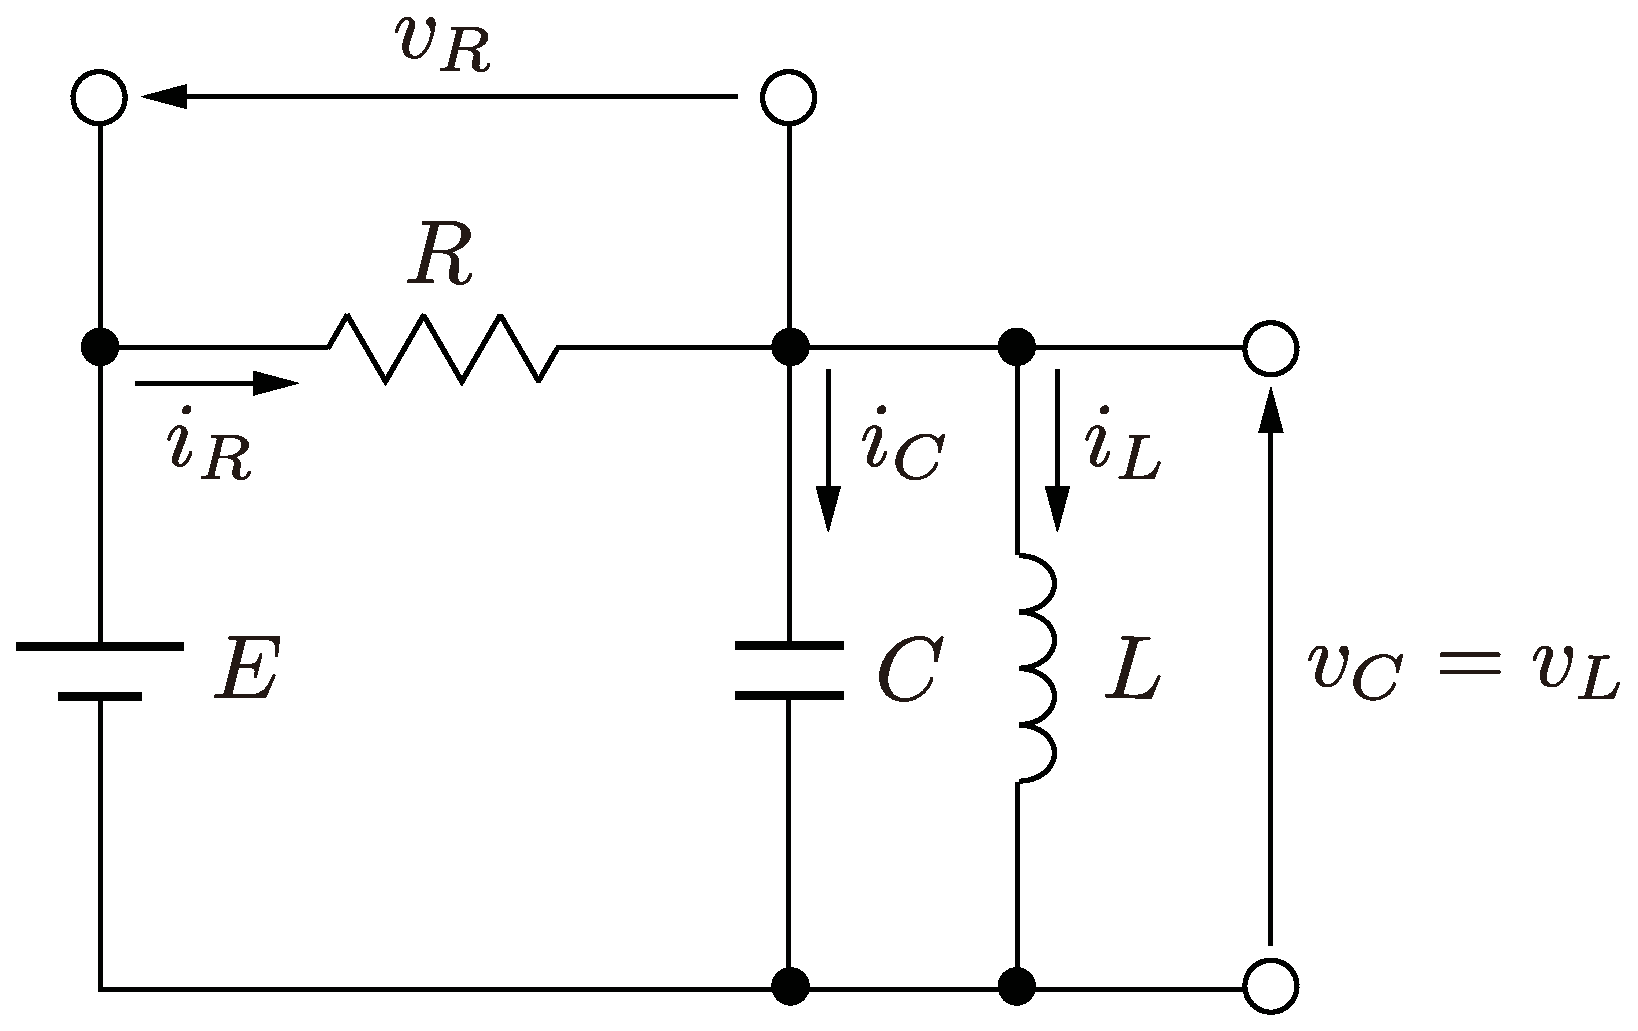
\includegraphics[width = .5\linewidth]{figs/circkawaguchi}
  \medskip
  \caption{\textbf{微分代数方程式の例題:LC並列回路}}
  \label{fig:RLC}
  \medskip
\end{figure}


\begin{例}[簡単な微分代数方程式系の数値解法]\label{ex:dae_ex1}
\FIGref{fig:RLC}に示される簡単な電気回路において,$R$,$L$,$C$,$E$がすべて1の場合の数値シミュレーションを行う。
この回路の動的な要素はコイル$L$とコンデンサ$C$であり,その微分方程式は
\begin{subequations}\label{eq:ex_de}
  \begin{align}
    L\dot i_L & = v_L \\
    C\dot v_C & = i_C
  \end{align}
\end{subequations}
である。ただし,初期値は$i_L(0)=0$,$v_C(0)=0$とする。
また,オームの法則とキルヒホッフの法則から
\begin{subequations}\label{eq:ex_ae}
  \begin{align}
    v_R & =R i_R      \\
    i_R & = i_L + i_C \\
    v_L & = v_C       \\
    E   & = v_C + v_R
  \end{align}
\end{subequations}
という代数方程式が成り立つ。

式(\ref{eq:ex_ae})の代数方程式を用いて$v_R$や$i_R$などの冗長な変数を消去すると,
等価な常微分方程式系を得ることができる。
この操作はクロン縮約に対応しており,得られる常微分方程式系は
\begin{subequations}\label{eq:ex1_ode}
  \begin{align}
    \dot{i}_L & = \frac{1}{L}v_C                     \\
    \dot{v}_C & = \frac{1}{RC}(E-v_C)-\frac{1}{C}i_L
  \end{align}
\end{subequations}
となる。まずは,この常微分方程式系を解くプログラムを書いてみよう。
常微分方程式系に対する\matlab のソルバは,\verb|ode45|が一般的である。
\verb|ode45|では,常微分方程式$\dot{x} = f(t, x)$
の関数$f(t, x)$を実装することにより常微分方程式系の解を求めることができる。
式(\ref{eq:ex1_ode})の右辺を実装すると,プログラム\ref{program:ex1_ode}のようになる。

\smallskip
\begin{PROGRAMA}[count,title={func\_RLC\_ode.m}]\label{program:ex1_ode}
  \begin{verbatim}
function dx = func_RLC_ode(x, R, C, L, E)

iL = x(1);
vC = x(2);

diL = vC/L;
dvC = (E-vC)/R/C - iL/C;

dx = [diL; dvC];

end
\end{verbatim}
\end{PROGRAMA}

これにより\verb|ode45|を実行して,常微分方程式系を解くとプログラム\nobreak\ref{program:main_ode1}となる。

\smallskip
\begin{PROGRAMA}[count,title={main\_RLC\_ode.m}]\label{program:main_ode1}
\begin{verbatim}
R = 1;
L = 1;
C = 1;
E = 1;

func = @(t, x) func_RLC_ode(x, R, C, L, E);
x0 = [0; 0];
tspan = [0 30];

[t, x] = ode45(func, tspan, x0);

plot(t, x)
\end{verbatim}
\end{PROGRAMA}

プログラム\nobreak\ref{program:main_ode1}における出力された変数\verb|x|は,$i_L$と$v_C$の時系列を縦に
並べた行列である。
したがって,$i_C$や$i_R$などの他の変数の時系列は,式(\ref{eq:ex_ae})の代数方程式を用いて追加で計算する必要があることに注意しよう。

つぎに,クロン縮約を介さず,微分代数方程式系の解を直接求めることを考える。
この場合には,物理的な代数方程式をそのまま書き下すことができるため,システムが複雑になっても記述が簡単であるという利点がある。
\matlab で微分代数方程式系を解くことができるコマンドの1つに\verb|ode15s|がある。
\verb|ode15s|は
\begin{align}\label{eq:numDAE}
  M\dot{x} = f(t, x)
\end{align}
という形式で記述された微分代数方程式系を対象とする。
式(\ref{eq:ex_de})と式(\ref{eq:ex_ae})をこの形にあてはめると
\[
\underbrace{
\mat{
    0 & L & 0 & 0 & 0 & 0 \\
    0 & 0 & 0 & 0 & 0 & C \\
    0 & 0 & 0 & 0 & 0 & 0 \\
    0 & 0 & 0 & 0 & 0 & 0 \\
    0 & 0 & 0 & 0 & 0 & 0 \\
    0 & 0 & 0 & 0 & 0 & 0 \\
}
}_{M}
\underbrace{
\mat{
    \dot i_R \\\dot i_L\\\dot i_C\\\dot v_R\\\dot v_L\\\dot v_C
}
}_{\dot{x}}
  =
\underbrace{
\mat{
    v_L \\i_C\\v_R-R i_R\\i_R-i_L-i_C\\v_L-v_C\\E-v_C-v_R
}
}_{f(t,x)}
\]
となる。ここで,右辺の3行目から6行目の要素を配置する順は任意であることに注意しよう。
この右辺を実装するとプログラム\ref{program:func_DAE1}となる。

\smallskip
\begin{PROGRAMA}[count,title={func\_RLC\_dae.m}]\label{program:func_DAE1}
\begin{verbatim}
function dx = func_RLC_dae(x, R, C, L, E)

iR = x(1);
iL = x(2);
iC = x(3);
vR = x(4);
vL = x(5);
vC = x(6);

diL = vL;
dvC = iC;

con1 = vC-vL;
con2 = E-vC-vR;
con3 = iR-(iC+iL);
con4 = vR-iR*R;

dx = [diL; dvC; con1; con2; con3; con4];
end
\end{verbatim}
\end{PROGRAMA}

この関数を用いると,プログラム\nobreak\ref{program:DAE1}のように微分代数方程式系を解くことができる。

\smallskip
\begin{PROGRAMA}[count,title={main\_RLC\_dae.m}]\label{program:DAE1}
\begin{verbatim}
R = 1;
C = 1;
L = 1;
E = 1;

M = zeros(6, 6);
M(1, 2) = L;
M(2, 6) = C;

x0 = zeros(6, 1);
tspan = [0 30];

options = odeset('Mass', M);
[t, x] = ode15s(@(t, x) func_RLC_dae(x, R, C, L, E),...
  tspan, x0, options);

plot(t, x(:, [2, 6]))
\end{verbatim}
\end{PROGRAMA}


このプログラムにおいて,13行目のオプションで式\ref{eq:numDAE}の$M$を設定している。
また,10行目で状態の初期値を設定しているが,
意味をもつのは微分方程式の状態,すなわち,2番目と6番目の要素のみである。
代数方程式の状態は,方程式を満たす値が\verb|ode15s|によって自動的に探索されるため,矛盾のない値をユーザ自身で計算して設定する必要はない。
実際,すべての要素を$0$とする初期値では代数方程式は満たされないが,微分代数方程式系の解は問題なく計算される。
15行目において得られる解\verb|x|は,$v_R, v_L, v_C, i_R, i_L, i_C$の時系列を並べた行列であり,
常微分方程式系に等価変換した場合と異なり,すべての変数の時系列が一度に求められる。

常微分方程式系に変換した場合と微分代数方程式系の解を直接計算した場合の$i_L$と$v_C$の時間応答を\FIGref{fig:solution_dae}
に示す。
それぞれの図には\verb|ode45|による解(青実線)と\verb|ode15s|による解(赤破線)の2本の線が表示されている。
明らかに,2つの解は等しい。


\begin{figure}[t]
  \centering
  {
    \begin{minipage}{0.49\linewidth}
      \centering
      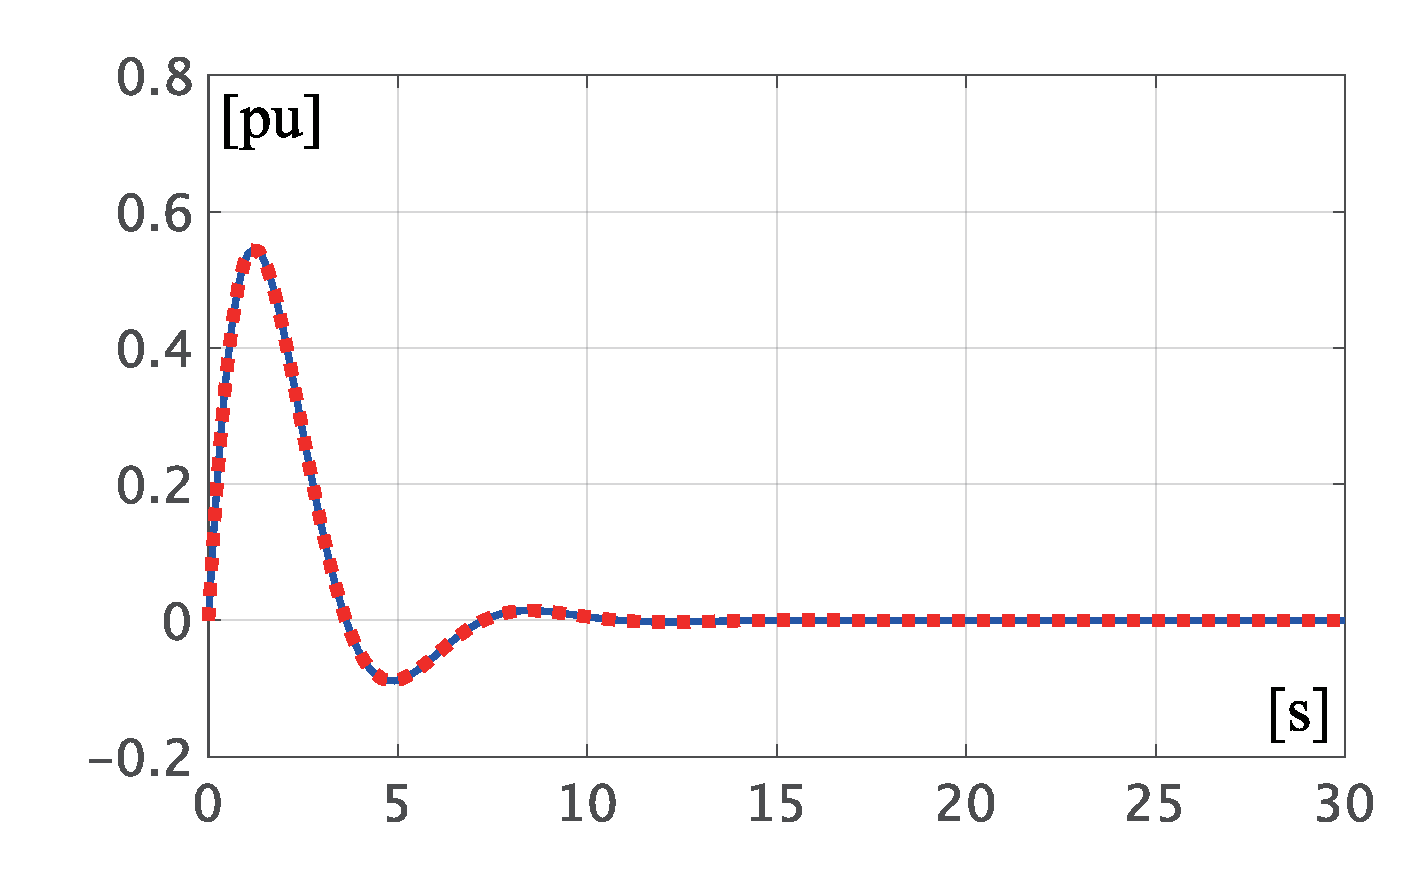
\includegraphics[width = 1.0\linewidth]{figs/iL}
      \subcaption{$i_L$の時間応答}
    \end{minipage}
    \begin{minipage}{0.49\linewidth}
      \centering
      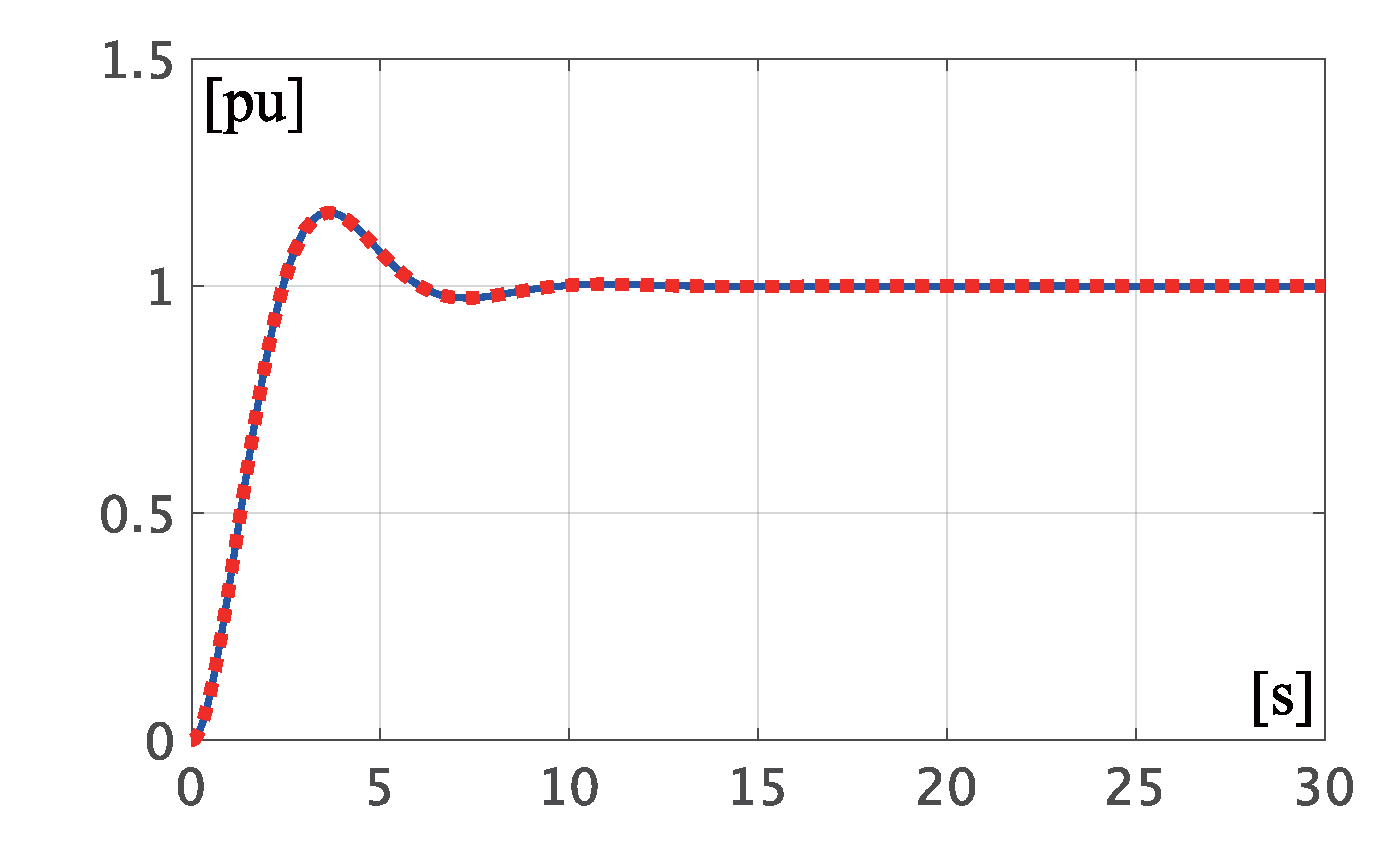
\includegraphics[width = 1.0\linewidth]{figs/vC}
      \subcaption{ $v_C$の時間応答}
    \end{minipage}
    \medskip
    \caption{\textbf{LC並列回路の時間応答}
      \\ \centering(青実線:ode45,赤破線:ode15s)}
    \label{fig:solution_dae}
  }
  \medskip
\end{figure}
\end{例}




\subsection{電力系統モデルの時間応答計算の単純な実装}

電力系統モデルの数値シミュレーションを実装する方法を説明する。

\begin{例}[電力系統のシミュレーションの単純な実装]\label{ex:dae_ex2}
例\ref{ex:inires}で扱った電力系統モデルの時間応答を数値計算するプログラムを実装しよう。
このシステムを記述するためには,発電機が接続された母線1と母線3について,\req{eq:gendynVIst}の微分方程式が必要である。
また,\req{eq:phVI}の代数方程式が成り立っている。
母線2には定インピーダンスの負荷モデルが接続されており,
\req{eq:cimp}の代数方程式が満たされている。
さらに,系統全体でキルヒホッフの法則である\req{eq:ohmY2}の代数方程式系が任意の時刻で成り立つ。

以下では,$\delta_1$,$\Delta\omega_1$,$E_1$,$\delta_3$,$\Delta\omega_3$,$E_3$,$\bm V_1$,$\bm V_2$,$\bm V_3$,$\bm I_1$,$\bm I_2$,$\bm I_3$を縦に並べたベクトルを$x$として
\[
M\dot{x} = f(t, x)
\]
の形式で記述することを考える。
右辺の関数$f(t, x)$の実装例は,プログラム\ref{program:simple_network_dae}となる。

\smallskip
\begin{PROGRAMA}[count,title={func\_simulation\_3bus.m}]\label{program:simple_network_dae}
\begin{verbatim}
function dx = func_simulation_3bus(x, Y, parameter)

delta1 = x(1);
omega1 = x(2);
E1 = x(3);
delta3 = x(4);
omega3 = x(5);
E3 = x(6);
V1 = x(7)  + 1j*x(8);
V2 = x(9)  + 1j*x(10);
V3 = x(11) + 1j*x(12);
I1 = x(13) + 1j*x(14);
I2 = x(15) + 1j*x(16);
I3 = x(17) + 1j*x(18);

omega0 = parameter.omega0;

X1 = parameter.X1;
X1_prime = parameter.X1_prime;
M1 = parameter.M1;
D1 = parameter.D1;
tau1 = parameter.tau1;
Pmech1 = parameter.Pmech1;
Vfield1 = parameter.Vfield1;

z2 = parameter.z2;

X3 = parameter.X3;
X3_prime = parameter.X3_prime;
M3 = parameter.M3;
D3 = parameter.D3;
tau3 = parameter.tau3;
Pmech3 = parameter.Pmech3;
Vfield3 = parameter.Vfield3;

P1 = real(V1*conj(I1));
P3 = real(V3*conj(I3));

dx1 = [omega0 * omega1;
    (-D1*omega1-P1+Pmech1)/M1;
    (-X1/X1_prime*E1+...
    (X1/X1_prime-1)*abs(V1)*cos(delta1-angle(V1))+Vfield1)/tau1];

dx3 = [omega0 * omega3;
    (-D3*omega3-P3+Pmech3)/M3;
    (-X3/X3_prime*E3+...
    (X3/X3_prime-1)*abs(V3)*cos(delta3-angle(V3))+Vfield3)/tau3];

con1 = I1-(E1*exp(1j*delta1)-V1)/(1j*X1_prime);
con2 = V2+z2*I2;
con3 = I3-(E3*exp(1j*delta3)-V3)/(1j*X3_prime);

con_network = [I1; I2; I3] - Y*[V1; V2; V3];

dx = [dx1; dx3;real(con1); imag(con1); real(con2);
    imag(con2); real(con3); imag(con3);
    real(con_network); imag(con_network)];

end
\end{verbatim}
\end{PROGRAMA}

このプログラムでは,\verb|x|に含まれる電圧フェーザや電流フェーザは,実部と虚部を並べて表現している。
また,変数をまとめて指定するために,構造体として\verb|parameter|を利用している。
プログラム\ref{program:simple_network_dae}を用いて微分代数方程式系を解くと
プログラム\nobreak\ref{program:main_simple_network_dae}となる。

\smallskip
\begin{PROGRAMA}[count,title={main\_simulation\_simple.m}]\label{program:main_simple_network_dae}
\begin{verbatim}
a_branch = cell(2, 1);
a_branch{1} = branch(1, 2, 1.3652-11.6040j);
a_branch{2} = branch(2, 3, -10.5107j);
Y = get_admittance_matrix(3, a_branch);

parameter = struct();

parameter.M1 = 100;
parameter.D1 = 10;
parameter.tau1 = 5.14;
parameter.X1 = 1.569;
parameter.X1_prime = 0.936;
parameter.Pmech1 = 2.5158;
parameter.Vfield1 = 2.7038;

parameter.z2 = 1.3224;

parameter.M3 = 12;
parameter.D3 = 10;
parameter.tau3 = 8.97;
parameter.X3 = 1.220;
parameter.X3_prime = 0.667;
parameter.Pmech3 = 0.5000;
parameter.Vfield3 = 2.1250;

parameter.omega0 = 60*2*pi;

x0 = [0.5357 + pi/6; 0; 2.3069 + 0.1;...
    0.0390; 0; 2.0654; zeros(12, 1)];
M = blkdiag(eye(6), zeros(12, 12));

tspan = [0 50];

options = odeset('Mass', M);
func = @(t, x) func_simulation_3bus(x, Y, parameter);
[t, x] = ode15s(func, tspan, x0, options); 

plot(t, x(:, [2, 5]))
\end{verbatim}
\end{PROGRAMA}

プログラム\nobreak\ref{program:main_simple_network_dae}では,
電力系統モデルの初期値応答を計算しており,2つの発電機の角周波数偏差が描画される。
\end{例}

\subsection{分割したモジュール群を用いた時間応答計算の実装法}

本節では,前節で述べたプログラムを機能ごとに分離し,拡張性の高いプログラムに変更する方法を説明する。

\begin{例}[発電機と負荷のモジュール化]\label{ex:gen_load}
  プログラム\nobreak\ref{program:simple_network_dae}は,
  入力された\verb|x|をそれぞれの機器の状態変数,電圧,電流に分割する処理と
  微分方程式や代数方程式を計算する処理という
  2つのステップから成り立っている。これらの2つを
 実行するプログラムを見通しよく記述する方法を考えよう。
 
  まず,変数\verb|x|を適切に分割するためには,各機器の状態数を把握する必要がある。
  また,すべての機器について,微分方程式における状態の時間微分$\tfrac{dx}{dt}$と代数方程式$f(x)=0$における$f(x)$の計算が行われている。
  ダックタイピングの考え方を用いれば,
  状態数を返す機能と時間微分,代数方程式の計算を行う機能をもてば,それを機器と定義して差し支えない。
  これらの機能をもつ機器として発電機と負荷を実装すると,プログラム\nobreak\ref{program:generator}とプログラム\ref{program:load}となる。

\smallskip
\begin{PROGRAMA}[count,title={generator.m}]\label{program:generator}
\begin{verbatim}
classdef generator < handle
  
properties
  omega0
  X
  X_prime
  M
  D
  tau
  Pmech
  Vfield
end

methods
  function obj = generator(omega0, M, D, tau,...
      X, X_prime, Pmech, Vfield)

    obj.omega0 = omega0;
    obj.X = X;
    obj.X_prime = X_prime;
    obj.M = M;
    obj.D = D;
    obj.tau = tau;
    obj.Pmech = Pmech;
    obj.Vfield = Vfield;
  end

  function nx = get_nx(obj)
    nx = 3;
  end

  function [dx, con] = get_dx_constraint(obj, x, V, I)
    delta = x(1);
    omega = x(2);
    E = x(3);
    P = real(V*conj(I));

    Pmech = obj.Pmech;
    Vfield = obj.Vfield;

    X = obj.X;
    X_prime = obj.X_prime;
    D = obj.D;
    M = obj.M;
    tau = obj.tau;

    omega0 = obj.omega0;

    dE = (-X/X_prime*E+...
      (X/X_prime-1)*abs(V)*cos(delta-angle(V))...
      +Vfield)/tau;
    dx = [omega0 * omega;
      (-D*omega-P+Pmech)/M;
      dE];
    con = I-(E*exp(1j*delta)-V)/(1j*X_prime);
    con = [real(con); imag(con)];
  end
end
  
end
\end{verbatim}
\end{PROGRAMA}


\smallskip
\begin{PROGRAMA}[count,title={load\_impedance.m}]\label{program:load}
\begin{verbatim}
classdef load_impedance < handle
  
properties
  z
end

methods
  function obj = load_impedance(z)
    obj.z = z;
  end

  function nx = get_nx(obj)
    nx = 0;
  end

  function [dx, con] = get_dx_constraint(obj, x, V, I)
    dx = [];
    z = obj.z;
    con = V+z*I;
    con = [real(con); imag(con)];
  end
end

end
\end{verbatim}
\end{PROGRAMA}

これらのプログラムでは,メソッドである\verb|get_nx|が
状態の数を返し,\verb|get_dx_constraint|が状態の時間微分と制約条件を返す。
このように定義された機器を用いると,プログラム\nobreak\ref{program:simple_network_dae}
は,プログラム\nobreak\ref{program:network_dae1}のように書き換えることができる。

\smallskip
\begin{PROGRAMA}[count,title={func\_simulation.m}]\label{program:network_dae1}
  \begin{verbatim}
function out = func_simulation(t, x, Y, a_component)

n_component = numel(a_component);
x_split = cell(n_component, 1);
V = zeros(n_component, 1);
I = zeros(n_component, 1);

idx = 0;
for k = 1:n_component
  nx = a_component{k}.get_nx();
  x_split{k} = x(idx+(1:nx));
  idx = idx + nx;
end

for k = 1:n_component
  V(k) = x(idx+1) + x(idx+2)*1j;
  idx = idx + 2;
end

for k = 1:n_component
  I(k) = x(idx+1) + x(idx+2)*1j;
  idx = idx + 2;
end

dx = cell(n_component, 1);
con = cell(n_component, 1);

for k = 1:n_component
  component = a_component{k};
  xk = x_split{k};
  Vk = V(k);
  Ik = I(k);
  [dx{k}, con{k}] = component.get_dx_constraint(xk, Vk, Ik);
end

con_network = I - Y*V;

out = vertcat(dx{:});
out = [out; vertcat(con{:})];
out = [out; real(con_network); imag(con_network)];

end
\end{verbatim}
\end{PROGRAMA}

プログラム\nobreak\ref{program:network_dae1}では,\verb|a_component|に機器のセル配列が入力されることを前提としている。
また,9行目から23行目で変数\verb|x|の分割を行っている。
このとき,10行目で機器の状態数を取得することにより,適切に分割を行うことができる。
28行目から34行目において,状態の時間微分と制約条件を計算する。
プログラムの33行目では,\verb|get_dx_constraint|を呼び出しており,
これは多態性を用いた実装となっている。
プログラムの38行目の\verb|vertcat(dx{:})|は,
セル配列\verb|dx|の要素をすべて垂直方向に結合している。
すなわち,
\verb|[dx{1}; dx{2}; ...; dx{end}]|に等しい。

プログラム\nobreak\ref{program:network_dae1}を用いて数値シミュレーションを実行することを考えよう。
具体的にプログラム\nobreak\ref{program:main_simple_network_dae}の数値シミュレーションに関する部分をまとめると,
プログラム\nobreak\ref{program:simulate_network1}のようになる。

\smallskip
\begin{PROGRAMA}[count,title={simulate\_power\_system.m}]\label{program:simulate_network1}
\begin{verbatim}
function [t, x, V, I] = ...
  simulate_power_system(a_component, Y, x0, tspan)

n_component = numel(a_component);
a_nx = zeros(n_component, 1);
for k = 1:n_component
  component = a_component{k};
  a_nx(k) = component.get_nx();
end
nx = sum(a_nx);

M = blkdiag(eye(nx), zeros(n_component*4));
options = odeset('Mass', M, 'RelTol', 1e-6);

y0 = [x0(:); zeros(4*n_component, 1)];

[t, y] = ode15s(@(t, x) func_simulation(t, x, Y, a_component),...
  tspan, y0, options);


x = cell(n_component, 1);
V = zeros(numel(t), n_component);
I = zeros(numel(t), n_component);

idx = 0;

for k = 1:n_component
  x{k} = y(:, idx+(1:a_nx(k)));
  Vk = y(:, nx+2*(k-1)+(1:2));
  V(:, k) = Vk(:, 1) + 1j*Vk(:, 2);
  Ik = y(:, nx+2*n_component+2*(k-1)+(1:2));
  I(:, k) = Ik(:, 1) + 1j*Ik(:, 2);
  idx = idx + a_nx(k);
end

end
\end{verbatim}
\end{PROGRAMA}

プログラム\nobreak\ref{program:simulate_network1}では,5行目から9行目で各機器から得た
状態の数を用いて,行列\verb|M|を定義している。
17行目ではプログラム\nobreak\ref{program:network_dae1}を用いて微分代数方程式を解いている。
27行目から34行目では,
計算結果を各機器の状態変数,各母線の電圧フェーザと電流フェーザに分割して返している。


さらに,プログラム\nobreak\ref{program:main_simple_network_dae}を書き換えると,プログラム\nobreak\ref{program:main_network1}となる。

\smallskip
\begin{PROGRAMA}[count,title={main\_simulation\_3bus.m}]\label{program:main_network1}
\begin{verbatim}
a_branch = cell(2, 1);
a_branch{1} = branch(1, 2, 1.3652-11.6040j);
a_branch{2} = branch(2, 3, -10.5107j);

Y = get_admittance_matrix(3, a_branch);

gen1 = generator(60*2*pi, 100, 10, 5.14,...
  1.569, 0.936, 2.5158, 2.7038);

load2 = load_impedance(1.3224);

gen3 = generator(60*2*pi, 12, 10, 8.97,...
  1.220, 0.667, 0.5000, 2.1250);

a_component = {gen1; load2; gen3};

x0 = [0.5357 + pi/6; 0; 2.3069 + 0.1; 0.0390; 0; 2.0654];
tspan = [0 50];

[t, x, V, I] = simulate_power_system(a_component, Y, x0, tspan);

plot(t, [x{1}(:, 2), x{3}(:, 2)])
\end{verbatim}
\end{PROGRAMA}

プログラム\nobreak\ref{program:main_network1}では,発電機や負荷を表す機器の配列\verb|a_component|
を作成して,プログラム\nobreak\ref{program:simulate_network1}で定義した関数\verb|simulate_power_system|を
実行している。
時間応答の数値計算において,送電網の構造や接続する機器を変更する場合には,プログラム
\ref{program:main_network1}の\verb|a_branch|と\verb|a_component|を変更すればよく,
プログラム\nobreak\ref{program:generator}からプログラム\ref{program:simulate_network1}を変更する必要はない。
また,プログラム\nobreak\ref{program:generator}やプログラム\ref{program:load}の発電機や負荷とは別の機器を用いる場合には,
\verb|get_nx|と\verb|get_dx_constraint|をもつクラスを実装して用いるだけでよい。
これらのモジュール化により,例\ref{ex:dae_ex2}の実装と比較して,可読性や拡張性が高いプログラムとなっている。

このプログラムの実行結果では,セル配列\verb|x|にそれぞれの機器の状態が返される。
この\verb|x|の要素が,それぞれの機器の状態変数の数と整合性のある行列となっていることを確認しよう。
ここで,母線2に接続された機器は負荷であり,状態の数は0であるため,\verb|x{2}|は0列の空行列となっている。
プログラムでは,母線1と母線3に接続された発電機の状態のうち2番目の要素,すなわち,角周波数偏差をプロットしている。
\end{例}

例\ref{ex:gen_load}では,発電機や負荷のモジュール化によって電力系統モデルの時間応答計算を見通しよく実装することができている。
ただし,プログラム\nobreak\ref{program:main_network1}では,発電機の外部入力や負荷のインピーダンスの値は,所望の平衡点に整合する値を事前に計算しておく必要がある。
これらの値はそれぞれの機器の動特性に依存するため,機能の分離の観点から改善の余地が残っている。
この問題を解決するために,例\ref{ex:gen_load}で述べたプログラムを拡張し,機能的により分離したプログラムとすることを考えよう。


\begin{例}[発電機や負荷の定常状態を計算するメソッドの追加]
電力系統モデルの時間応答の数値計算において,所望の電力供給を実現する定常潮流状態を達成することを考える。
このとき,発電機と負荷のそれぞれで,式(\ref{eq:intssgen})と式\ref{eq:lmodimppara}が満たされる必要がある。
これらの関係式は,各機器の状態方程式と関連しているため,\verb|generator|や\verb|load_impedance|のクラスに実装するのが適切である。
この観点から,プログラム\ref{program:generator}とプログラム\ref{program:load}に
所望の電力需給を達成する定常状態を計算するメソッドを追加するとプログラム\nobreak\ref{program:generator2}とプログラム\ref{program:load2}となる。

\smallskip
\begin{PROGRAMA}[count,title={generator.m}]\label{program:generator2}
  \begin{verbatim}
classdef generator < handle
  
(プログラム3-23の3行目から12行目と同じ)

methods

(プログラム3-23の15行目から57行目と同じ)

  function x_equilibrium = set_equilibrium(obj, V, I, P, Q)
    Vabs = abs(V);
    Vangle = angle(V);
    
    X = obj.X;
    X_prime = obj.X_prime;
    
    delta = Vangle + atan(P/(Q+Vabs^2/X_prime));
    E = X_prime/Vabs*sqrt((Q+Vabs^2/X_prime)^2+P^2);
    
    x_equilibrium = [delta; 0; E];
    
    obj.Pmech = P;
    obj.Vfield = X*E/X_prime ...
      - (X/X_prime-1)*Vabs*cos(delta-Vangle);
  end

end
  
end
\end{verbatim}
\end{PROGRAMA}

\smallskip
\begin{PROGRAMA}[count,title={load\_impedance.m}]\label{program:load2}
\begin{verbatim}
classdef load_impedance < handle
  
(プログラム3-24の3行目から5行目と同じ)

methods
  
(プログラム3-24の8行目から21行目と同じ)

  function x_equilibrium = set_equilibrium(obj, V, I, P, Q)
    x_equilibrium = [];
    obj.z = -V/I;
  end

end

end
\end{verbatim}
\end{PROGRAMA}
これらのプログラムにおいて,\verb|set_equilibrium|は所望の定常状態における母線の電圧フェーザ
\verb|V|,電流フェーザ\verb|I|,有効電力\verb|P|,無効電力\verb|Q|を受け取り,状態の定常値\verb|x_equilibrium|を
返すメソッドである。
ここで,理論的には\verb|I|を与える必要はなく,\verb|V|と\verb|P|
のみで十分であるが,利便性のために\verb|I|も与えている。
潮流計算で得られたパラメータを用いて,例\ref{ex:gen_load}と同様のシミュレーションを行うプログラムは,つぎのように記述することができる。

\smallskip
\begin{PROGRAMA}[count,title={main\_simulation\_3bus\_equilibrium.m}]\label{program:main_equilibrium}
\begin{verbatim}
a_bus = cell(3, 1);
a_bus{1} = bus_slack(2, 0);
a_bus{2} = bus_load(-3, 0);
a_bus{3} = bus_generator(0.5, 2);

a_branch = cell(2, 1);
a_branch{1} = branch(1, 2, 1.3652-11.6040j);
a_branch{2} = branch(2, 3, -10.5107j);

gen1 = generator(60*2*pi, 100, 10, 5.14, 1.569, 0.936, [], []);
load2 = load_impedance([]);
gen3 = generator(60*2*pi, 12, 10, 8.97, 1.220, 0.667, [], []);

a_component = {gen1; load2; gen3};

[V, I, P, Q] = calculate_power_flow(a_bus, a_branch);
Y = get_admittance_matrix(3, a_branch);

x_equilibrium = cell(numel(a_component), 1);
for k=1:numel(a_component)
   x_equilibrium{k} =...
     a_component{k}.set_equilibrium(V(k), I(k), P(k), Q(k)); 
end

x0 = vertcat(x_equilibrium{:});
x0(1) = x0(1) + pi/6;
x0(3) = x0(3) + 0.1;
tspan = [0 50];

[t, x, V, I] = simulate_power_system(a_component, Y, x0, tspan);

plot(t, [x{1}(:, 2), x{3}(:, 2)])
\end{verbatim}
\end{PROGRAMA}

プログラム\ref{program:main_equilibrium}では,母線,送電線,発電機,負荷
のクラスを利用して電力系統モデルを定義して潮流計算を行い,時間応答を計算するという一連のプロセスが明瞭となっている。
ユーザは,各機器の物理定数を指定するだけで,内部の動特性などに注意を払わずに数値シミュレーションを実行することができる。
この例では,機器のモデルが\verb|set_equilibrium|というメソッドをもつことを前提としている。
これは,ダックタイピングにおける機器の定義を変更していることに相当する。
\end{例}

以上の例では,電力系統モデルの初期値応答の数値計算を扱ってきた。
つぎに,地絡に対する時間応答計算の実装法について述べる。

\begin{例}[地絡に対する時間応答の数値計算]
地絡に対する応答を計算するためには,\ref{sec:fault}節で述べたように,
地絡が生じた母線の電圧を一定時間$0$に固定すればよい。
これは,プログラム\nobreak\ref{program:network_dae1}の36行目の制約条件を一部変更することによって,つぎのように実装できる。

\smallskip
\begin{PROGRAMA}[count,title={func\_simulation.m}]\label{program:network_dae_fault}
\begin{verbatim}
function out = func_simulation(t, x, Y, a_component, bus_fault)

(プログラム3-25の3行目から34行目と同じ)

con_network = I - Y*V;
con_network(bus_fault) = V(bus_fault);

(プログラム3-25の38行目から40行目と同じ)

end
\end{verbatim}
\end{PROGRAMA}

このプログラムでは,入力引数が追加されており,\verb|bus_fault|に地絡が生じる母線の番号を代入することが想定されている。
この変更に対応させてプログラム\nobreak\ref{program:simulate_network1}を変更するとプログラム\ref{program:simulate_network2}となる。

\smallskip
\begin{PROGRAMA}[count,title={simulate\_power\_system.m}]\label{program:simulate_network2}
  \begin{verbatim}
function [t, x, V, I] = simulate_power_system(a_component, ...
  Y, x0, tspan,bus_fault, tspan_fault)

if nargin < 5
  bus_fault = [];
end

if nargin < 6
  tspan_fault = [0, 0];
end

(プログラム3-26の4行目から15行目と同じ)

if isempty(bus_fault)
  [t, y] = ode15s(...
    @(t, x) func_simulation(t, x, Y, a_component, []),...
    tspan, y0, options);
else
  [t1, y1] = ode15s(...
    @(t, x) func_simulation(t, x, Y, a_component, bus_fault),...
  tspan_fault, y0, options);
  
  [t2, y2] = ode15s(...
    @(t, x) func_simulation(t, x, Y, a_component, []),...
  [tspan_fault(2), tspan(2)], y1(end, :), options);

  t = [t1; t2];
  y = [y1; y2];
end

(プログラム3-26の21行目から34行目と同じ)

end
\end{verbatim}
\end{PROGRAMA}

このプログラムでは,入力引数に地絡が生じる母線と時間区間が追加されている。
ただし,4行目から10行目では,これらの値が入力されなかった場合のデフォルト値を設定しているため,
プログラム\nobreak\ref{program:main_network1}と同様に地絡を指定せずに利用することもできる。
このような過去のプログラムが新しいバージョンでも利用できる性質は,\textbf{後方互換性}(backward compatibility)\index{ こうほうごかんせい@後方互換性}と呼ばれる。

プログラム\nobreak\ref{program:simulate_network2}では,19行目から21行目で地絡を指定しており,地絡が解消された後の数値シミュレーションを23行目から25行目で実行している。
このとき,地絡が解消された後の数値シミュレーションにおける状態の初期値は,地絡中の時間応答計算の最終値としていることに注意されたい。
このプログラムを用いて地絡に対する時間応答を数値シミュレーションするプログラムを記述するとプログラム\nobreak\ref{program:main_fault}となる。

\smallskip
\begin{PROGRAMA}[count,title={main\_simulation\_3bus\_fault.m}]\label{program:main_fault}
\begin{verbatim}

(プログラム3-30の1行目から23行目と同じ)

x0 = vertcat(x_equilibrium{:});
tspan = [0 50];

fault_bus = 1;
fault_tspan = [0, 50e-3];

[t, x, V, I] = simulate_power_system(a_component, Y, x0, tspan,...
  fault_bus, fault_tspan);

plot(t, [x{1}(:, 2), x{3}(:, 2)])
\end{verbatim}
\end{PROGRAMA}

このプログラムを実行すると,\ref{fig:P3faulta}に相当する結果が得られる。
\end{例}

さいごに,入力信号に対する時間応答の計算法を述べる。

\begin{例}[入力信号に対する時間応答の数値計算]
これまで扱ってきた例において,発電機の機械入力$P_\mathrm{mech}$を変化させることや,例\ref{sec:resldpara}のように負荷の大きさを変化させる数値シミュレーションを行うことを考える。
このために,外部入力を考慮できるようにプログラムを変更する。

外部入力を考慮するためには,各機器が受け取る入力の数が明示されていることが必要である。
この観点から,機器の定義に「入力の数を返すメソッドがあること」を追加する。
さらに,状態変数の時間微分や制約条件の計算に外部入力を反映させるように
プログラム\ref{program:generator2}と\ref{program:load2}を修正すると,プログラム\ref{program:generator3}とプログラム\ref{program:load3}となる。

\smallskip
\begin{PROGRAMA}[count,title={generator.m}]\label{program:generator3}
  \begin{verbatim}
classdef generator < handle
  
(プログラム3-23の3行目から12行目と同じ)

methods

(プログラム3-23の15行目から30行目と同じ)

  function nu = get_nu(obj)
    nu = 1;
  end

  function [dx, con] = get_dx_constraint(obj, x, V, I, u)
    
(プログラム3-23の33行目から36行目と同じ)

    Pmech = obj.Pmech + u;

(プログラム3-23の39行目から56行目と同じ)

  end

(プログラム3-28の9行目から24行目と同じ)

end
end
\end{verbatim}
\end{PROGRAMA}

\begin{PROGRAMA}[count,title={load\_impedance.m}]\label{program:load3}
\begin{verbatim}
classdef load_impedance < handle
  
(プログラム3-24の3行目から5行目と同じ)

methods

(プログラム3-24の8行目から21行目と同じ)
  
  function nu = get_nu(obj)
    nu = 2;
  end

  function [dx, con] = get_dx_constraint(obj, x, V, I, u)
    dx = [];
    z = real(obj.z)*(1+u(1)) + 1j*imag(obj.z)*(1+u(2));
    con = V+z*I;
    con = [real(con); imag(con)];
  end

(プログラム3-29の9行目から12行目と同じ)

end

end
\end{verbatim}
\end{PROGRAMA}

これらプログラムでは,\verb|get_nu|が受け取ることができる入力の数を返している。
また,\verb|get_dx_constraint|が入力\verb|u|を受け取って適切な処理するように変更されている。
このとき,発電機に対する入力は$P_\mathrm{mech}$の増分を表しており,負荷に対する入力はインピーダンスの実部と虚部の変化の割合を表している。
これらの機器を使って入力応答が計算できるようにプログラム\ref{program:network_dae_fault}と\ref{program:simulate_network2}
を修正するとプログラム\ref{program:network_dae_input}と\ref{program:simulate_network3}となる。

\smallskip
\begin{PROGRAMA}[count,title={func\_simulation.m}]\label{program:network_dae_input}
\begin{verbatim}
function out = func_simulation(t, x, Y, a_component,...
  bus_fault, U, bus_U)

(プログラム3-25の3行目から26行目と同じ)

for k = 1:n_component

(プログラム3-25の29行目から32行目と同じ)
  
  if ismember(k, bus_U)
    uk = U{bus_U==k}(t);
  else
    uk = zeros(component.get_nu(), 1);
  end
  
  [dx{k}, con{k}] = component.get_dx_constraint(xk, Vk, Ik, uk);
  
end

(プログラム3-31の5行目から6行目と同じ)

(プログラム3-25の38行目から40行目と同じ)

end
\end{verbatim}
\end{PROGRAMA}

\begin{PROGRAMA}[count,title={simulate\_power\_system.m}]\label{program:simulate_network3}
\begin{verbatim}
function [t, x, V, I] = simulate_power_system(a_component, ...
  Y, x0, tspan,bus_fault, tspan_fault, U, bus_U)

(プログラム3-32の4行目から10行目と同じ)

if nargin < 7
    U = {};
    bus_U = [];
end

(プログラム3-26の4行目から15行目と同じ)

if isempty(bus_fault)
  func = @(t, x) func_simulation(t, x, Y, a_component,...
    [], U, bus_U);
  [t, y] = ode15s(func, tspan, y0, options);
else
  func = @(t, x) func_simulation(t, x, Y, a_component,...
    bus_fault, U, bus_U);
  [t1, y1] = ode15s(func, tspan_fault, y0, options);
  
  func = @(t, x) func_simulation(t, x, Y, a_component,...
    [], U, bus_U);
  [t2, y2] = ode15s(func, ...
    [tspan_fault(2), tspan(2)], y1(end, :), options);
  
  t = [t1; t2];
  y = [y1; y2];
end
(プログラム3-26の21行目から34行目と同じ)

end
\end{verbatim}
\end{PROGRAMA}

これらのプログラムでは,入力引数に\verb|U|と\verb|bus_U|が
追加されている。
ここで,\verb|bus_U|には入力信号を指定する母線の番号が代入されることを想定している。
また,\verb|U|は指定された母線の数の要素をもつセル配列である。
その要素は時刻\verb|t|を受け取り,入力信号を返す関数である。
プログラム\ref{program:network_dae_input}の11行目では,
\verb|U|のうち,\verb|k|番目の母線に対応する要素を探し出していることに注意する。

変更された関数を用いてシミュレーションを行うプログラムを例示したものがプログラム\nobreak\ref{program:main_input}である。

\smallskip
\begin{PROGRAMA}[count,title={main\_simulation\_3bus\_input.m}]\label{program:main_input}
\begin{verbatim}

  (プログラム3-30の1行目から25行目と同じ)

tspan = [0 50];

bus_U = [1; 2];
U = {@(t) 0; @(t) [0.05*t/50; 0.05*t/50]};

[t, x, V, I] = simulate_power_system(a_component, Y, x0,...
    tspan, [], [], U, bus_U);

plot(t, [x{1}(:, 2), x{3}(:, 2)])
\end{verbatim}
\end{PROGRAMA}

プログラム\nobreak\ref{program:main_input}では,6行目と7行目で入力信号を定義している。
このプログラムでは,負荷のインピーダンスを50秒間で5\%増加させている。
母線1の入力信号は常に0を返すものであるため意味をもたないが,指定方法を例示するために追加した。
また,母線3には入力を指定していないが,この場合には自動的に0が入力される。
以上のプログラムの変更により,外部入力に対する時間応答計算を行うことができる。
この変更は後方互換性を保つことに留意されているため,
プログラム\nobreak\ref{program:main_input}を適切に書き換えることで,
様々な電力系統に対する初期値応答や地絡や外部入力に対する時間応答を計算することができる。
このとき,プログラム\nobreak\ref{program:main_input}を除く他のプログラム群は一切の変更を加えずに利用することができる。
これがモジュール群に分割した実装の利点である。
\end{例}


\section*{数学的補足}

\begin{補題}\label{lem:sumc}
実定数$r_i$,$\omega_i$,$\phi_i$に対して
\begin{align*}
\bm{C}_n(t) := 
\sum_{i=1}^n r_i e^{ \bm{j} (\omega_i t + \phi_i)}
\end{align*}
とする。
ただし,$r_i>0$および$\phi_i \in [0,2\pi)$とする。
このとき,$\bm{C}_1$が$t$に依らない定数であるための必要十分条件は$\omega_1=0$である。
また,$\bm{C}_2$が$t$に依らない定数であるための必要十分条件は
$\omega_1=\omega_2=0$または
\begin{align*}
\omega_1=\omega_2
,\qquad
r_1=r_2
,\qquad
|\phi_2-\phi_1| = \pi
\end{align*}
である。
さらに,$\omega_1$,$\omega_2$,$\omega_3$がすべて0でないとき,$\bm{C}_3$が$t$に依らない定数であるための必要十分条件は
\begin{align*}
\omega_1=\omega_2=\omega_3
,\qquad
\sum_{i=1}^3 r_i e^{\bm{j}\phi_i}=0
\end{align*}
である。
\end{補題}

\begin{証明}
まず,$\bm{C}_1$の$t$に関する微分を0と置くことで
\begin{align*}
r_1 \omega_1 e^{ \bm{j} (\omega_1 t + \phi_1)}=0
\end{align*}
を得る。
したがって,$\bm{C}_1$が$t$に依らない定数であることの必要十分条件は,$\omega_1=0$である。
つぎに,$\bm{C}_2$の$t$に関する微分を0と置くことで
\begin{align}\label{eq:C2d}
r_1 \omega_1 e^{ \bm{j} (\omega_1 t + \phi_1)}
+ r_2 \omega_2 e^{ \bm{j} (\omega_2 t + \phi_2)}=0
\end{align}
を得る。
両辺に$e^{ -\bm{j} (\omega_1 t + \phi_1)}$を掛けてさらに$t$で微分すると
\begin{align*}
r_2 \omega_2 (\omega_2-\omega_1)
e^{ \bm{j} \left\{ 
(\omega_2-\omega_1) t + \phi_2 - \phi_1)
\right\}
}=0
\end{align*}
が得られる。
これは
$\omega_2 (\omega_2-\omega_1)=0$
と等価である。
したがって,$\omega_1 =\omega_2$が得られる。
特に,$\omega_1=\omega_2=0$である場合には,任意の$r_1$,$r_2$,$\phi_1$,$\phi_1$に対して,式\ref{eq:C2d}は満たされる。
また,$\omega_1$と$\omega_2$が0でないとき,式\ref{eq:C2d}は
\begin{align*}
r_1 e^{ \bm{j} \phi_1} + r_2 e^{ \bm{j} \phi_2} =0
\end{align*}
と等価であることがわかる。
これは$r_1=r_2$かつ$|\phi_2-\phi_1| = \pi$と等価である。

さいごに,$\bm{C}_3$について考える。
これまでと同様に,$\bm{C}_2$の$t$に関する微分を0と置くことで
\begin{align}\label{eq:C3d}
r_1 \omega_1 e^{ \bm{j} (\omega_1 t + \phi_1)}
+ r_2 \omega_2 e^{ \bm{j} (\omega_2 t + \phi_2)}
+ r_3 \omega_3 e^{ \bm{j} (\omega_3 t + \phi_3)}=0
\end{align}
を得る。
両辺に$e^{ -\bm{j} (\omega_1 t + \phi_1)}$を掛けてさらに$t$で微分すると
\begin{align*}
r_2 \omega_2 (\omega_2-\omega_1)
e^{ \bm{j} \left\{ 
(\omega_2-\omega_1) t + \phi_2 - \phi_1)
\right\}
} +
r_3 \omega_3 (\omega_3-\omega_1)
e^{ \bm{j} \left\{ 
(\omega_3-\omega_1) t + \phi_3 - \phi_1)
\right\}
}=0
\end{align*}
が得られる。
同様に,両辺に$e^{ -\bm{j} \{(\omega_2-\omega_1) t + \phi_2 - \phi_1\}}$を掛けてさらに$t$で微分すると
\begin{align*}
r_3 \omega_3 (\omega_3-\omega_1) (\omega_3-\omega_2)
e^{ \bm{j} \left\{ 
(\omega_3-\omega_2) t + \phi_3 - \phi_2)
\right\}
}=0
\end{align*}
が得られる。
これは,$\omega_3\neq0$であることから
\begin{subequations}\label{eq:omegas}
\begin{align}
(\omega_3-\omega_1) (\omega_3-\omega_2)=0
\end{align}
と等価である。
同様の手順により,式\ref{eq:C3d}から
\begin{align}
(\omega_2-\omega_1) (\omega_3-\omega_2)=0
,\qquad
(\omega_3-\omega_1) (\omega_2-\omega_1)=0
\end{align}
\end{subequations}
が得られる。
式\ref{eq:omegas}は$\omega_1=\omega_2=\omega_3$と等価である。
このとき,$\omega_1$,$\omega_2$,$\omega_3$が0でないことから,式\ref{eq:C3d}と
\begin{align*}
\sum_{i=1}^n r_i e^{\bm{j}\phi_i}
=0
\end{align*}
が等価であることが導かれる。
\end{証明}


\end{document}
%\red{(以下、不要かも)}
%
%さいごに,以上の議論から導かれるつぎの事実を示す。
%
%\begin{定理}[母線変数の計測による母線同期の判定]
%\label{cor:PQsync}
%式\ref{eq:PQVgen}の連立方程式によって機器群が結合された電力系統モデルを考える。
%電力系統は定常潮流状態にあるものと仮定する。
%このとき,次数2の母線$i$に対して
%\begin{align}\label{eq:PQnot2}
%P_i \neq \real[\bm{Y}_{ii}] |\bm{V}_i|^2
%\qquad
%{\rm または}
%\qquad
%Q_i \neq - \imag [\bm{Y}_{ii}] |\bm{V}_i|^2
%\end{align}
%が成り立つ,もしくは,その隣接母線に対して
%\begin{align}\label{eq:VYnot2}
%\spliteq{
%& |\bm{V}_{j_1}| |\bm{Y}_{ij_1}| \neq 
%|\bm{V}_{j_2}| |\bm{Y}_{ij_2}|
%\qquad
%{\rm または} \\
%& |\angle \bm{V}_{j_1} - \angle \bm{V}_{j_2} - \angle \bm{Y}_{ij_1} + \angle \bm{Y}_{ij_2} | \neq \pi
%}
%\end{align}
%が成り立つならば,式\ref{eq:alloms}が成り立つ。
%ただし,$\mathcal{N}_i = \{j_1,j_2\}$である。
%また,次数3の母線$i$に対して,$\Omega_i = \Omega_{j_3}$を満たす$j_3 \in \mathcal{N}_i$が存在するものとする。
%このとき,母線$i$に対して
%\begin{align}\label{eq:PQnot3}
%\spliteq{
% P_i  &\neq \real[\bm{Y}_{ii}] |\bm{V}_i|^2  + |\bm{Y}_{ij_3}| |\bm{V}_i| |\bm{V}_{j_3}| 
%\sfcos (\angle \bm{V}_i - \angle \bm{V}_{j_3} - \angle \bm{Y}_{ij_3}) \\
%& \hspace{6em} {\rm または} 
%\\
%Q_i & \neq - \imag [\bm{Y}_{ii}] |\bm{V}_i|^2  + |\bm{Y}_{ij_3}| |\bm{V}_i| |\bm{V}_{j_3}| 
%\sfsin (\angle \bm{V}_i - \angle \bm{V}_{j_3} - \angle \bm{Y}_{ij_3})
%}
%\end{align}
%が成り立つ,もしくは,その隣接母線に対して式\ref{eq:VYnot2}が成り立つならば,式\ref{eq:alloms}が成り立つ。
%ただし,$ \mathcal{N}_i \setminus \{j_3\}=\{j_1,j_2\}$である。
%\end{定理}
%
%\begin{証明}
%次数2の母線に関する題意を対偶により示す。
%すなわち,式\ref{eq:alloms}の否定,すなわち,式\ref{eq:N2sing}が成り立つならば,式\ref{eq:PQnot2}や式\ref{eq:VYnot2}の否定が成り立つことを示す。
%まず,式\ref{eq:VYnot2}の否定は,式\ref{eq:N2sing}の中央と右そのものであることから,後者の含意は明らかである。
%つぎに,式\ref{eq:N2sing}が成り立つとき,式\ref{eq:sumcirc}の$\bm{c}_i$は0であることが導かれる。
%これは,式\ref{eq:PQnot2}の否定,すなわち
%\begin{align*}
%P_i = \real[\bm{Y}_{ii}] |\bm{V}_i|^2
%,\qquad
%Q_i = - \imag [\bm{Y}_{ii}] |\bm{V}_i|^2
%\end{align*}
%を意味する。
%以上より,次数2の母線に関する題意が示される。
%次数3の母線に関する題意も同様に示される。
%\end{証明}
%
%
%定理\ref{cor:PQsync}により,有効電力や無効電力,電圧フェーザを実際に計測することによって,グラフ構造だけでは判断できなかった母線の同期を示すことが可能となる。
%例えば,\FIGref{fig:hony}(b)のハニカム構造をもつ送電網に対して,定常潮流状態において適当な母線の有効電力や無効電力,電圧フェーザを計測し,いずれかの赤と青の母線の同期を示すことができれば,送電網全体での母線の同期が結論できる。
%




%\bibliographystyle{myjunsrt}		% bib style
%\bibliography{reference_corona,referencejp}	% your bib database


\newpage
\end{document}